%%% Verze pro jednostranný tisk:
\documentclass[11pt,a4paper]{report}
\usepackage[top=25mm,bottom=25mm,right=25mm,left=30mm,head=12.5mm,foot=12.5mm]{geometry}
\let\openright=\clearpage

%%% Pokud tiskneme oboustranně:
%\documentclass[11pt,a4paper,twoside,openright]{report}
%\usepackage[top=25mm,bottom=25mm,right=25mm,left=30mm,head=12.5mm,foot=12.5mm]{geometry}
%\let\openright=\cleardoublepage

%%% Definice různých užitečných maker (viz popis uvnitř souboru)
%%% Tento soubor obsahuje definice různých užitečných maker a prostředí %%%
%%% Další makra připisujte sem, ať nepřekáží v ostatních souborech.     %%%
%%% This file contains definitions of various useful macros and environments      %%%
%%% Assign additional macros here so that they do not interfere with other files. %%%

\usepackage[a-2u]{pdfx}     % výsledné PDF bude ve standardu PDF/A-2u
                            % resulting PDF will be in the PDF / A-2u standard

\usepackage{ifpdf}
\usepackage{ifxetex}
\usepackage{ifluatex}
\usepackage{minted}
\usepackage{xcolor}

%%% Nastavení pro použití samostatné bibliografické databáze.
%%% Settings for using a separate bibliographic database.
\usepackage[
   backend=biber
  ,style=iso-authoryear
  % ,style=iso-numeric
  % ,sortlocale=cs_CZ
  ,alldates=iso
  ,bibencoding=UTF8
  ,maxnames=2
  ,maxbibnames=99
  %,block=ragged
]{biblatex}
\let\cite\parencite
\renewcommand*{\multinamedelim}{, \addspace}
\renewcommand*{\finalnamedelim}{\addspace a \addspace}

\bibliography{literatura}

%% Přepneme na českou sazbu, fonty Latin Modern a kódování češtiny
\ifthenelse{\boolean{xetex}\OR\boolean{luatex}}
   { % use fontspec and OpenType fonts with utf8 engines
			\usepackage[english,slovak,czech]{babel}
			\usepackage[autostyle,english=british,czech=quotes]{csquotes}
			\usepackage{fontspec}
			\defaultfontfeatures{Ligatures=TeX,Scale=MatchLowercase}
   }
   {
			\usepackage[english,slovak,czech]{babel}
			\usepackage{lmodern}
			\usepackage[T1]{fontenc}
			\usepackage{textcomp}
			\usepackage[utf8]{inputenc}
			\usepackage[autostyle,english=british,czech=quotes]{csquotes}
	 }
\ifluatex
\makeatletter
\let\pdfstrcmp\pdf@strcmp
\makeatother
\fi

%%% Další užitečné balíčky (jsou součástí běžných distribucí LaTeXu)
\usepackage{amsmath}        % rozšíření pro sazbu matematiky / extension for math typesetting
\usepackage{amsfonts}       % matematické fonty / mathematical fonts
\usepackage{amssymb}        % symboly / symbols
\usepackage{amsthm}         % sazba vět, definic apod. / typesetting of sentences, definitions, etc.
\usepackage{bm}             % tučné symboly (příkaz \bm) / bold symbols (\bm command)
\usepackage{graphicx}       % vkládání obrázků / graphics inserting
\usepackage{listings}       % vylepšené prostředí pro strojové písmo / improved environment for source codes typesetting
\usepackage{fancyhdr}       % prostředí pohodlnější nastavení hlavy a paty stránek / environment for more comfortable adjustment of the head and foot of the pages
\usepackage{icomma}         % inteligetní čárka v matematickém módu / intelligent comma in math mode
\usepackage{dcolumn}        % lepší zarovnání sloupců v tabulkách / better alignment of columns in tables
\usepackage{booktabs}       % lepší vodorovné linky v tabulkách / better horizontal lines in tables
\makeatletter
\@ifpackageloaded{xcolor}{
   \@ifpackagewith{xcolor}{usenames}{}{\PassOptionsToPackage{usenames}{xcolor}}
  }{\usepackage[usenames]{xcolor}} % barevná sazba / color typesetting
\makeatother
\usepackage{multicol}       % práce s více sloupci na stránce / work with multiple columns on a page
\usepackage{caption}
\usepackage{enumitem}
\setlist[itemize]{noitemsep, topsep=0pt, partopsep=0pt}
\setlist[enumerate]{noitemsep, topsep=0pt, partopsep=0pt}
\setlist[description]{noitemsep, topsep=0pt, partopsep=0pt}

\usepackage{hyperref}
\usepackage{float}
\usepackage[section]{placeins}

\usepackage{tocloft}
\setlength\cftparskip{0pt}
\setlength\cftbeforechapskip{1.5ex}
\setlength\cftfigindent{0pt}
\setlength\cfttabindent{0pt}
\setlength\cftbeforeloftitleskip{0pt}
\setlength\cftbeforelottitleskip{0pt}
\setlength\cftbeforetoctitleskip{0pt}
\renewcommand{\cftlottitlefont}{\Huge\bfseries\sffamily}
\renewcommand{\cftloftitlefont}{\Huge\bfseries\sffamily}
\renewcommand{\cfttoctitlefont}{\Huge\bfseries\sffamily}

\clubpenalty = 10000
\widowpenalty = 10000
\raggedbottom

% vyznaceni odstavcu
% differentiation of new paragraphs
\parindent=0pt
\parskip=11pt

% zakaz vdov a sirotku - jednoradkovych pocatku ci koncu odstavcu na prechodu mezi strankami
% Prohibition of widows and orphans - single-line beginning and end of paragraph at the transition between pages
\clubpenalty=1000
\widowpenalty=1000
\displaywidowpenalty=1000

% nastaveni radkovani
% setting of line spacing
\renewcommand{\baselinestretch}{1.20}

% nastaveni pro nadpisy - tucne a bezpatkove
% settings for headings - bold and sans serif
\usepackage{sectsty}    
\allsectionsfont{\sffamily}

% nastavení hlavy a paty stránek
% page head and foot settings
\makeatletter
\if@twoside%
    \fancypagestyle{fancyx}{%
            \fancyhf{}                                     
      \fancyhead[RE]{\rightmark}                  
      \fancyhead[LO]{\leftmark}                  
      \fancyfoot[RO,LE]{\thepage}                    
      \renewcommand{\headrulewidth}{.5pt}            
      \renewcommand{\footrulewidth}{.5pt}            
    }
    \fancypagestyle{plain}{%
            \fancyhf{}                                     
        \fancyfoot[RO,LE]{\thepage}                    
        \renewcommand{\headrulewidth}{0pt}             
        \renewcommand{\footrulewidth}{0.5pt}
    }          
\else
    \fancypagestyle{fancyx}{%
        \fancyhf{}                                     
        \fancyhead[R]{\nouppercase{\leftmark}}
        \fancyfoot[R]{\thepage}                    
        \renewcommand{\headrulewidth}{.5pt}            
        \renewcommand{\footrulewidth}{.5pt}            
    }
    \fancypagestyle{plain}{%                       
        \fancyhf{} % clear all header and footer fields
        \fancyfoot[R]{\thepage}                    
        \renewcommand{\headrulewidth}{0pt}             
        \renewcommand{\footrulewidth}{0.5pt}
    }
    
% nastavení hlavy a paty stránek
% page head and foot settings
% \makeatletter
% \if@twoside%
%     \fancypagestyle{fancyx}{%
% 			\fancyhf{}                                     
%       \fancyhead[RE]{\rightmark}                  
%       \fancyhead[LO]{\leftmark}                  
%       \fancyfoot[RO,LE]{\thepage}                    
%       \renewcommand{\headrulewidth}{.5pt}            
%       \renewcommand{\footrulewidth}{.5pt}            
%     }
%     \fancypagestyle{plain}{%
% 			\fancyhf{}                                     
%     	\fancyfoot[RO,LE]{\thepage}                    
%     	\renewcommand{\headrulewidth}{0pt}             
%     	\renewcommand{\footrulewidth}{0.5pt}
%     }          
% \else
%     \fancypagestyle{fancyx}{%
% 			\fancyhf{}                                     
%       \fancyhead[R]{\leftmark}                  
%       \fancyfoot[R]{\thepage}                    
%       \renewcommand{\headrulewidth}{.5pt}            
%       \renewcommand{\footrulewidth}{.5pt}            
%     }
%     \fancypagestyle{plain}{%                       
%     	\fancyhf{} % clear all header and footer fields
%     	\fancyfoot[R]{\thepage}                    
%     	\renewcommand{\headrulewidth}{0pt}             
%     	\renewcommand{\footrulewidth}{0.5pt}
%     }          
\fi
\renewcommand*{\cleardoublepage}{\clearpage\if@twoside \ifodd\c@page\else
	\hbox{}%
	\thispagestyle{empty}%
	\newpage%
	\if@twocolumn\hbox{}\newpage\fi\fi\fi
}
\makeatother

% Tato makra přesvědčují mírně ošklivým trikem LaTeX, aby hlavičky kapitol
% sázel příčetněji a nevynechával nad nimi spoustu místa. Směle ignorujte.
% These macros convince with a slightly ugly LaTeX trick to make chapter headers
% bet more sane and didn't miss a lot of space above them. Be boldly ignore it.
\makeatletter
\def\@makechapterhead#1{
  {\parindent \z@ \raggedright \sffamily
   \Huge\bfseries \thechapter. #1
   \par\nobreak
   \vskip 20\p@
}}
\def\@makeschapterhead#1{
  {\parindent \z@ \raggedright \sffamily
   \Huge\bfseries #1
   \par\nobreak
   \vskip 20\p@
}}
\makeatother

% Trochu volnější nastavení dělení slov, než je default.
% Slightly looser hyphenation setting than default.
\lefthyphenmin=2
\righthyphenmin=2

% Zapne černé "slimáky" na koncích řádků, které přetekly, abychom si jich lépe všimli.
% Turns on the black "snails" at the ends of the lines that overflowed to get us noticed them better.
\overfullrule=1mm

%% Balíček hyperref, kterým jdou vyrábět klikací odkazy v PDF,
%% ale hlavně ho používáme k uložení metadat do PDF (včetně obsahu).
%% Většinu nastavítek přednastaví balíček pdfx.
%% A hyperref package that can be used to produce clickable links in PDF,
%% but we mainly use it to store metadata in PDF (including content).
%% Most settings are preset by the pdfx package.
\hypersetup{unicode}
\hypersetup{breaklinks=true}
\hypersetup{hidelinks}

\renewcommand{\UrlBreaks}{\do\/\do\=\do\+\do\-\do\_\do\ \do\a\do\b\do\c\do\d%
\do\e\do\f\do\g\do\h\do\i\do\j\do\k\do\l\do\m\do\n\do\o\do\p\do\q\do\r\do\s%
\do\t\do\u\do\v\do\w\do\x\do\y\do\z\do\A\do\B\do\C\do\D\do\E\do\F\do\G\do\H%
\do\I\do\J\do\K\do\L\do\M\do\N\do\O\do\P\do\Q\do\R\do\S\do\T\do\U\do\V\do\W%
\do\X\do\Y\do\Z\do\1\do\2\do\3\do\4\do\5\do\6\do\7\do\8\do\9\do\0}

%%% Prostředí pro sazbu kódu, případně vstupu/výstupu počítačových
%%% programů. (Vyžaduje balíček listings -- fancy verbatim.)
%%% Environment for source code typesetting, or computer input/output
%%% programs. (Requires package listings - fancy verbatim.)
% \lstnewenvironment{code}{\lstset{basicstyle=\small, frame=single}}{}
\definecolor{bg}{rgb}{0.95,0.95,0.92}
\renewcommand{\lstlistingname}{Výpis}
\lstdefinestyle{default}{
  basicstyle=\ttfamily\footnotesize\selectlanguage{czech},
  backgroundcolor=\color{bg},
  breakatwhitespace=false,         
  breaklines=true,                 
  captionpos=t,                    
  keepspaces=true,                 
  numbersep=5pt,                  
  showspaces=false,                
  showstringspaces=false,
  showtabs=false,                  
  tabsize=2,
  literate={
      {á}{{\'a}}1 {é}{{\'e}}1 {í}{{\'i}}1 {ó}{{\'o}}1 {ú}{{\'u}}1 {ý}{{\'y}}1
      {Á}{{\'A}}1 {É}{{\'E}}1 {Í}{{\'I}}1 {Ó}{{\'O}}1 {Ú}{{\'U}}1 {Ý}{{\'Y}}1
      {ř}{{{\v{r}}}}1 {ž}{{{\v{z}}}}1 {č}{{{\v{c}}}}1 {š}{{{\v{s}}}}1 {ě}{{{\v{e}}}}1 
      {Ř}{{{\v{R}}}}1 {Ž}{{{\v{Z}}}}1 {Č}{{{\v{C}}}}1 {Š}{{{\v{S}}}}1 {Ě}{{{\v{E}}}}1 
      {ů}{{\r{u}}}1 {€}{{\EUR}}1 {£}{{\pounds}}1
  }
}
\lstset{style=default}

\newcommand{\code}{\texttt}

\newcommand{\todo}[1]{\colorbox{pink}{\if\relax\detokenize{#1}\relax TODO\else TODO: #1\fi}}
\newcommand{\imgsource}[1]{}
\newcommand{\imagesource}[1]{}

\DeclareCiteCommand{\tcite}
  {\usebibmacro{prenote}}%
  {\usebibmacro{citeindex}%
   \usebibmacro{cite}%
   \marginpar{\usebibmacro{sidecite}}}
  {\multicitedelim}
  {\usebibmacro{postnote}}

\newcommand{\customcite}[2]{\hyperlink{cite.\therefsection @#1}{#2 \protect\NoHyper\cite*{#1}\protect\endNoHyper}}

%%% DEFINICE ZÁKLADNÍCH PROMĚNNÝCH
\def\TypPrace{BP}                % bakalářská práce/bachelor thesis
%\def\TypPrace{DP}               % diplomová práce/master thesis
\def\Jazyk{cze}                  % čeština/czech
%\def\Jazyk{slo}                 % slovenština/slovak
%\def\Jazyk{eng}                 % angličtina/english

%%% Název práce v jazyce práce (přesně podle zadání)
%%% Title of the thesis in the language used in the text (exact according to assignment)
\def\NazevPrace{Webové rozšíření přidávající funkcionalitu do informačního systému InSIS}

%%% Tento soubor obsahuje definice různých užitečných maker a prostředí %%%
%%% Další makra připisujte sem, ať nepřekáží v ostatních souborech.     %%%
%%% This file contains definitions of various useful macros and environments      %%%
%%% Assign additional macros here so that they do not interfere with other files. %%%

\usepackage[a-2u]{pdfx}     % výsledné PDF bude ve standardu PDF/A-2u
                            % resulting PDF will be in the PDF / A-2u standard

\usepackage{ifpdf}
\usepackage{ifxetex}
\usepackage{ifluatex}
\usepackage{minted}
\usepackage{xcolor}

%%% Nastavení pro použití samostatné bibliografické databáze.
%%% Settings for using a separate bibliographic database.
\usepackage[
   backend=biber
  ,style=iso-authoryear
  % ,style=iso-numeric
  % ,sortlocale=cs_CZ
  ,alldates=iso
  ,bibencoding=UTF8
  ,maxnames=2
  ,maxbibnames=99
  %,block=ragged
]{biblatex}
\let\cite\parencite
\renewcommand*{\multinamedelim}{, \addspace}
\renewcommand*{\finalnamedelim}{\addspace a \addspace}

\bibliography{literatura}

%% Přepneme na českou sazbu, fonty Latin Modern a kódování češtiny
\ifthenelse{\boolean{xetex}\OR\boolean{luatex}}
   { % use fontspec and OpenType fonts with utf8 engines
			\usepackage[english,slovak,czech]{babel}
			\usepackage[autostyle,english=british,czech=quotes]{csquotes}
			\usepackage{fontspec}
			\defaultfontfeatures{Ligatures=TeX,Scale=MatchLowercase}
   }
   {
			\usepackage[english,slovak,czech]{babel}
			\usepackage{lmodern}
			\usepackage[T1]{fontenc}
			\usepackage{textcomp}
			\usepackage[utf8]{inputenc}
			\usepackage[autostyle,english=british,czech=quotes]{csquotes}
	 }
\ifluatex
\makeatletter
\let\pdfstrcmp\pdf@strcmp
\makeatother
\fi

%%% Další užitečné balíčky (jsou součástí běžných distribucí LaTeXu)
\usepackage{amsmath}        % rozšíření pro sazbu matematiky / extension for math typesetting
\usepackage{amsfonts}       % matematické fonty / mathematical fonts
\usepackage{amssymb}        % symboly / symbols
\usepackage{amsthm}         % sazba vět, definic apod. / typesetting of sentences, definitions, etc.
\usepackage{bm}             % tučné symboly (příkaz \bm) / bold symbols (\bm command)
\usepackage{graphicx}       % vkládání obrázků / graphics inserting
\usepackage{listings}       % vylepšené prostředí pro strojové písmo / improved environment for source codes typesetting
\usepackage{fancyhdr}       % prostředí pohodlnější nastavení hlavy a paty stránek / environment for more comfortable adjustment of the head and foot of the pages
\usepackage{icomma}         % inteligetní čárka v matematickém módu / intelligent comma in math mode
\usepackage{dcolumn}        % lepší zarovnání sloupců v tabulkách / better alignment of columns in tables
\usepackage{booktabs}       % lepší vodorovné linky v tabulkách / better horizontal lines in tables
\makeatletter
\@ifpackageloaded{xcolor}{
   \@ifpackagewith{xcolor}{usenames}{}{\PassOptionsToPackage{usenames}{xcolor}}
  }{\usepackage[usenames]{xcolor}} % barevná sazba / color typesetting
\makeatother
\usepackage{multicol}       % práce s více sloupci na stránce / work with multiple columns on a page
\usepackage{caption}
\usepackage{enumitem}
\setlist[itemize]{noitemsep, topsep=0pt, partopsep=0pt}
\setlist[enumerate]{noitemsep, topsep=0pt, partopsep=0pt}
\setlist[description]{noitemsep, topsep=0pt, partopsep=0pt}

\usepackage{hyperref}
\usepackage{float}
\usepackage[section]{placeins}

\usepackage{tocloft}
\setlength\cftparskip{0pt}
\setlength\cftbeforechapskip{1.5ex}
\setlength\cftfigindent{0pt}
\setlength\cfttabindent{0pt}
\setlength\cftbeforeloftitleskip{0pt}
\setlength\cftbeforelottitleskip{0pt}
\setlength\cftbeforetoctitleskip{0pt}
\renewcommand{\cftlottitlefont}{\Huge\bfseries\sffamily}
\renewcommand{\cftloftitlefont}{\Huge\bfseries\sffamily}
\renewcommand{\cfttoctitlefont}{\Huge\bfseries\sffamily}

\clubpenalty = 10000
\widowpenalty = 10000
\raggedbottom

% vyznaceni odstavcu
% differentiation of new paragraphs
\parindent=0pt
\parskip=11pt

% zakaz vdov a sirotku - jednoradkovych pocatku ci koncu odstavcu na prechodu mezi strankami
% Prohibition of widows and orphans - single-line beginning and end of paragraph at the transition between pages
\clubpenalty=1000
\widowpenalty=1000
\displaywidowpenalty=1000

% nastaveni radkovani
% setting of line spacing
\renewcommand{\baselinestretch}{1.20}

% nastaveni pro nadpisy - tucne a bezpatkove
% settings for headings - bold and sans serif
\usepackage{sectsty}    
\allsectionsfont{\sffamily}

% nastavení hlavy a paty stránek
% page head and foot settings
\makeatletter
\if@twoside%
    \fancypagestyle{fancyx}{%
            \fancyhf{}                                     
      \fancyhead[RE]{\rightmark}                  
      \fancyhead[LO]{\leftmark}                  
      \fancyfoot[RO,LE]{\thepage}                    
      \renewcommand{\headrulewidth}{.5pt}            
      \renewcommand{\footrulewidth}{.5pt}            
    }
    \fancypagestyle{plain}{%
            \fancyhf{}                                     
        \fancyfoot[RO,LE]{\thepage}                    
        \renewcommand{\headrulewidth}{0pt}             
        \renewcommand{\footrulewidth}{0.5pt}
    }          
\else
    \fancypagestyle{fancyx}{%
        \fancyhf{}                                     
        \fancyhead[R]{\nouppercase{\leftmark}}
        \fancyfoot[R]{\thepage}                    
        \renewcommand{\headrulewidth}{.5pt}            
        \renewcommand{\footrulewidth}{.5pt}            
    }
    \fancypagestyle{plain}{%                       
        \fancyhf{} % clear all header and footer fields
        \fancyfoot[R]{\thepage}                    
        \renewcommand{\headrulewidth}{0pt}             
        \renewcommand{\footrulewidth}{0.5pt}
    }
    
% nastavení hlavy a paty stránek
% page head and foot settings
% \makeatletter
% \if@twoside%
%     \fancypagestyle{fancyx}{%
% 			\fancyhf{}                                     
%       \fancyhead[RE]{\rightmark}                  
%       \fancyhead[LO]{\leftmark}                  
%       \fancyfoot[RO,LE]{\thepage}                    
%       \renewcommand{\headrulewidth}{.5pt}            
%       \renewcommand{\footrulewidth}{.5pt}            
%     }
%     \fancypagestyle{plain}{%
% 			\fancyhf{}                                     
%     	\fancyfoot[RO,LE]{\thepage}                    
%     	\renewcommand{\headrulewidth}{0pt}             
%     	\renewcommand{\footrulewidth}{0.5pt}
%     }          
% \else
%     \fancypagestyle{fancyx}{%
% 			\fancyhf{}                                     
%       \fancyhead[R]{\leftmark}                  
%       \fancyfoot[R]{\thepage}                    
%       \renewcommand{\headrulewidth}{.5pt}            
%       \renewcommand{\footrulewidth}{.5pt}            
%     }
%     \fancypagestyle{plain}{%                       
%     	\fancyhf{} % clear all header and footer fields
%     	\fancyfoot[R]{\thepage}                    
%     	\renewcommand{\headrulewidth}{0pt}             
%     	\renewcommand{\footrulewidth}{0.5pt}
%     }          
\fi
\renewcommand*{\cleardoublepage}{\clearpage\if@twoside \ifodd\c@page\else
	\hbox{}%
	\thispagestyle{empty}%
	\newpage%
	\if@twocolumn\hbox{}\newpage\fi\fi\fi
}
\makeatother

% Tato makra přesvědčují mírně ošklivým trikem LaTeX, aby hlavičky kapitol
% sázel příčetněji a nevynechával nad nimi spoustu místa. Směle ignorujte.
% These macros convince with a slightly ugly LaTeX trick to make chapter headers
% bet more sane and didn't miss a lot of space above them. Be boldly ignore it.
\makeatletter
\def\@makechapterhead#1{
  {\parindent \z@ \raggedright \sffamily
   \Huge\bfseries \thechapter. #1
   \par\nobreak
   \vskip 20\p@
}}
\def\@makeschapterhead#1{
  {\parindent \z@ \raggedright \sffamily
   \Huge\bfseries #1
   \par\nobreak
   \vskip 20\p@
}}
\makeatother

% Trochu volnější nastavení dělení slov, než je default.
% Slightly looser hyphenation setting than default.
\lefthyphenmin=2
\righthyphenmin=2

% Zapne černé "slimáky" na koncích řádků, které přetekly, abychom si jich lépe všimli.
% Turns on the black "snails" at the ends of the lines that overflowed to get us noticed them better.
\overfullrule=1mm

%% Balíček hyperref, kterým jdou vyrábět klikací odkazy v PDF,
%% ale hlavně ho používáme k uložení metadat do PDF (včetně obsahu).
%% Většinu nastavítek přednastaví balíček pdfx.
%% A hyperref package that can be used to produce clickable links in PDF,
%% but we mainly use it to store metadata in PDF (including content).
%% Most settings are preset by the pdfx package.
\hypersetup{unicode}
\hypersetup{breaklinks=true}
\hypersetup{hidelinks}

\renewcommand{\UrlBreaks}{\do\/\do\=\do\+\do\-\do\_\do\ \do\a\do\b\do\c\do\d%
\do\e\do\f\do\g\do\h\do\i\do\j\do\k\do\l\do\m\do\n\do\o\do\p\do\q\do\r\do\s%
\do\t\do\u\do\v\do\w\do\x\do\y\do\z\do\A\do\B\do\C\do\D\do\E\do\F\do\G\do\H%
\do\I\do\J\do\K\do\L\do\M\do\N\do\O\do\P\do\Q\do\R\do\S\do\T\do\U\do\V\do\W%
\do\X\do\Y\do\Z\do\1\do\2\do\3\do\4\do\5\do\6\do\7\do\8\do\9\do\0}

%%% Prostředí pro sazbu kódu, případně vstupu/výstupu počítačových
%%% programů. (Vyžaduje balíček listings -- fancy verbatim.)
%%% Environment for source code typesetting, or computer input/output
%%% programs. (Requires package listings - fancy verbatim.)
% \lstnewenvironment{code}{\lstset{basicstyle=\small, frame=single}}{}
\definecolor{bg}{rgb}{0.95,0.95,0.92}
\renewcommand{\lstlistingname}{Výpis}
\lstdefinestyle{default}{
  basicstyle=\ttfamily\footnotesize\selectlanguage{czech},
  backgroundcolor=\color{bg},
  breakatwhitespace=false,         
  breaklines=true,                 
  captionpos=t,                    
  keepspaces=true,                 
  numbersep=5pt,                  
  showspaces=false,                
  showstringspaces=false,
  showtabs=false,                  
  tabsize=2,
  literate={
      {á}{{\'a}}1 {é}{{\'e}}1 {í}{{\'i}}1 {ó}{{\'o}}1 {ú}{{\'u}}1 {ý}{{\'y}}1
      {Á}{{\'A}}1 {É}{{\'E}}1 {Í}{{\'I}}1 {Ó}{{\'O}}1 {Ú}{{\'U}}1 {Ý}{{\'Y}}1
      {ř}{{{\v{r}}}}1 {ž}{{{\v{z}}}}1 {č}{{{\v{c}}}}1 {š}{{{\v{s}}}}1 {ě}{{{\v{e}}}}1 
      {Ř}{{{\v{R}}}}1 {Ž}{{{\v{Z}}}}1 {Č}{{{\v{C}}}}1 {Š}{{{\v{S}}}}1 {Ě}{{{\v{E}}}}1 
      {ů}{{\r{u}}}1 {€}{{\EUR}}1 {£}{{\pounds}}1
  }
}
\lstset{style=default}

\newcommand{\code}{\texttt}

\newcommand{\todo}[1]{\colorbox{pink}{\if\relax\detokenize{#1}\relax TODO\else TODO: #1\fi}}
\newcommand{\imgsource}[1]{}
\newcommand{\imagesource}[1]{}

\DeclareCiteCommand{\tcite}
  {\usebibmacro{prenote}}%
  {\usebibmacro{citeindex}%
   \usebibmacro{cite}%
   \marginpar{\usebibmacro{sidecite}}}
  {\multicitedelim}
  {\usebibmacro{postnote}}

\newcommand{\customcite}[2]{\hyperlink{cite.\therefsection @#1}{#2 \protect\NoHyper\cite*{#1}\protect\endNoHyper}}

%%% Jméno autora
%%% Author's name - First name Surname
\def\AutorPrace{Jiří Vrba}

%%% Rok odevzdání a měsíc (slovně)
%%% Year of submission and month (verbally) - month YYYY
\def\DatumOdevzdani{květen 2023}

%%% Vedoucí práce: Jméno a příjmení s~tituly
%%% Supervisor: First name and surname with titles
\def\Vedouci{Ing. Jiří Sedláček, Ph.D.}

%%% Konzultant práce: Jméno a příjmení s~tituly
%%% Consultant: First name and surname with titles
\def\Konzultant{}

%%% Studijní program
%%% Study program
\def\StudijniProgram{Aplikovaná informatika}

%%% Studijní program - specializace
%%% Study program - specialization
\def\Specializace{}

%%% Studijní obor
%%% Field of study
\def\StudijniObor{}

%%% Nepovinné poděkování (vedoucímu práce, konzultantovi, tomu, kdo zapůjčil software, literaturu apod.)
%%% Optional thanks (the supervisor, the consultant, the borrower of software, literature, etc.)
\def\Podekovani{%
Poděkování.
}

%%% Abstrakt (doporučený rozsah cca 150-250 slov; nejedná se o zadání práce)
\def\Abstrakt{%
Abstrakt.
}
\def\AbstraktEN{%
Abstract.
}

%%% 3 až 5 klíčových slov (doporučeno)
\def\KlicovaSlova{klíčové slovo, další pojem, jiný důležitý termín, a ještě jeden}
\def\KlicovaSlovaEN{keyword, important term, another topic, and another one}


%%% Titulní strana a různé povinné informativní strany
%%% Title page and various mandatory information pages
\begin{document}
%%% Titulní strana práce a další povinné informační strany

%%% Titulní strana práce

\pagestyle{empty}
\hypersetup{pageanchor=false}

\begin{center}
\Huge\sffamily
\VSE\\
\FIS

\vspace{\stretch{1}}

\ifstringequal{\Jazyk}{eng}{
	
\includegraphics[width=.5\textwidth]{img/FIS_2_logo_2_rgb_EN}
}{
	
\includegraphics[width=.5\textwidth]{img/FIS_2_logo_2_rgb_CZ}
}

\vspace{\stretch{2}}

\bfseries\NazevPrace

\vspace{8mm}
\mdseries\TypPraceText

\vspace{8mm}
\large
\begin{tabular}{rl}
\StudijniProgramText: & \StudijniProgram \\
\ifthenelse{\equal{\Specializace}{}}{%
	% empty value
	}{
	\rule{0pt}{6mm}%
	\SpecializaceText: & \Specializace \\
}
\ifthenelse{\equal{\StudijniObor}{}}{%
	% empty value
	}{
	\rule{0pt}{6mm}%
	\StudijniOborText: & \StudijniObor \\
}
\end{tabular}

\vspace{\stretch{8}}

\begin{tabular}{rl}
\AutorText: & \AutorPrace \\
\noalign{\vspace{2mm}}
\VedouciText: & \Vedouci \\
\ifthenelse{\equal{\Konzultant}{}}{%
	% empty value
	}{
	\rule{0pt}{6mm}%
	\KonzultantText: & \Konzultant \\
}
\end{tabular}

\vspace{8mm}
\Praha, \DatumOdevzdani
\end{center}


%%% Poděkování
\hypersetup{pageanchor=true}
\cleardoublepage
\pagestyle{plain}
\openright
\vspace*{\fill}
\section*{\PodekovaniText}
\noindent
\Podekovani
\vspace{1cm}


%%% Povinná informační strana práce
\openright
\section*{Abstrakt}
\noindent
\Abstrakt
\subsection*{Klíčová slova}
\noindent
\KlicovaSlova

\bigskip\bigskip\bigskip\bigskip\bigskip
\section*{Abstract}
\noindent
\AbstraktEN
\subsection*{Keywords}
\noindent
\KlicovaSlovaEN

\openright


%%% Strana s automaticky generovaným obsahem práce
%%% A page with automatically generated content of the thesis
\setcounter{tocdepth}{2}
\tableofcontents

%%% Seznam obrázků v práci
%%% List of figures in the thesis
\openright
\listoffigures
Poznámka: Seznam obrázků je vhodný použít, pokud počet obrázků v textu práce je větší než 20. Seznam grafů je vhodný použít pouze v případě, že autor práce rozlišuje mezi obrázkem a grafem. Seznam grafů je utvářen, pokud je počet grafů větší než 20. V této šabloně závěrečné práce se grafy a obrázky nerozlišují.

%%% Seznam tabulek v práci (volitelně)
%%% List of tables in the thesis (optionally)
\clearpage
\listoftables
Poznámka: Seznam tabulek je vhodný použít, pokud počet tabulek v textu práce je větší než 20.

%%% Seznam zkratek v práci (volitelně)
%%% List of abbreviations in the thesis (optionally)
\chapter*{\SeznamZkratek}

\begin{multicols}{2}
\raggedright
\begin{description}
% \item [BCC] Blind Carbon Copy
% \item [CC] Carbon Copy
% \item [CERT] Computer Emergency Response Team
% \item [CSS] Cascading Styleheets
% \item [DOI] Digital Object Identifier
% \item [REST] Representational State Transfer
% \item [SOAP] Simple Object Access Protocol
% \item [URI] Uniform Resource Identifier
% \item [URL] Uniform Resource Locator
\item [AJAX] Asynchronous JavaScript and XML
\item [API] Application Programming Interface
\item [CD] Continuous Delivery
\item [CI] Continuous Integration
\item [CLR] Common Language Runtime
\item [CRUD] Create, Read, Update, Delete
\item [DTO] Data Transfer Object
\item [HTML] Hypertext Markup Language
\item [HTTP] Hyper Text Transfer Protocol
\item [JSON] JavaScript Object Notation
\item [JVM] Java Virtual Machine
\item [NPM] Node Package Manager
\item [REST] Representational State Transfer
\item [SQL] Structured Query Language
\item [UI] User Interface
\item [URL] Uniform Resource Locator
\item [UX] User Experience
\item [XML] eXtended Markup Language
\end{description}
\end{multicols}

% Poznámka: Seznam zkratek je vhodný použít, pokud počet zkratek v textu práce je větší než 20 a nejedná se o zkratky běžné.

\pagestyle{fancyx}
%%% Jednotlivé kapitoly práce jsou pro přehlednost uloženy v samostatných souborech
%%% The individual chapters of the thesis are stored in separate files for clarity
{%
\pagestyle{plain}
\chapter*{Úvod}
\addcontentsline{toc}{chapter}{Úvod}

Během svého studia na Vysoké škole ekonomické v~Praze všichni studenti přijdou do styku se školním informačním systémem InSIS. Tento informační systém obsahuje širokou škálu modulů a funkcionalit, se kterými studenti během svého studia na vysoké škole pracují.

Ačkoliv tento systém poskytuje svým uživatelům všechny potřebné informace, přidáním některých funkcionalit by bylo možné zlepšit produktivitu uživatelů tohoto systému a celkově zpříjemnit studium studentů.

Tato práce si klade za cíl vymezit a následně implementovat rozšiřující funkcionality do informačního systému InSIS, které následně budou distribuovány v~podobě rozšíření do webových prohlížečů. Součástí práce je zároveň implementace podpůrného webového serveru, který poskytuje REST API pro uživatele rozšíření. Dalším cílem práce je popis výběru technologií použitých pro implementací obou softwarových částí produktu. Posledním cílem je evaluace zpětné vazby od ostatních studentů a ověření stanovených hypotéz.

Motivací pro tuto práci byla negativní zkušenost autora a jeho spolužáků s~používáním některých modulů školního informačního systému InSIS. 
Současné podobě této práce předcházela sada uživatelských skriptů naprogramovaných autorem v~průběhu studia, které má tato práce za cíl nahradit a naimplementovat nové, rozšiřující funkcionality do informačního systému InSIS v~podobě koherentního softwarového řešení, které bude jednoduché na instalaci a používání.

Práce je dělena do celkem pěti částí: 

\begin{enumerate}
    \item Návrh a popisem implementovaných funkcionalit,
    \item Proces výběru technologií použitých pro implementaci,
    \item Implementace podpůrného webového serveru
    \item Implementace rozšíření do webových prohlížečů
    \item Evaluace zpětné vazby od ostatních studentů, kteří webové rozšíření používají
\end{enumerate}

Práce se zaměřuje především na praktickou problematiku spojenou s~implementací softwarového řešení s~výjimkou první a poslední části, které jsou zaměřené více teoreticky.

Výsledkem práce by mělo být kompletně implementované, publikované rozšíření do webových prohlížečů založených na technologii Google Chrome a webový prohlížeč Mozilla Firefox.

% Úvod je povinnou částí bakalářské/diplomové práce. Úvod je uvedením do tématu. Zvolené téma rozvádí, stručně ho zasazuje do souvislostí (může zde být i popis motivace k sepsání práce) a odpovídá na otázku, proč bylo téma zvoleno. Zasazuje téma do souvislostí a zdůvodňuje jeho nutnost a aktuálnost řešení. Obsahuje explicitně uvedený cíl práce. Text cíle práce je shodný s textem, který je uveden v zadání bakalářské práce, tj. s textem, který je uveden v systému InSIS a který je také uveden v části Abstrakt.

% Součástí úvodu je také stručné představení postupu zpracování práce (detailně je metodě zpracování věnována samostatná část vlastního textu práce). Úvod může zahrnovat i popis motivace k sepsání práce.

% Úvod k diplomové práci musí být propracovanější -- podrobněji to je uvedeno v Náležitostech diplomové práce v rámci Intranetu pro studenty FIS.

% Následuje několik ukázkových kapitol, které doporučují, jak by se měla bakalářská/diplomová práce sázet. Primárně popisují použití \TeX{}ové šablony, ale obecné rady poslouží dobře i~uživatelům jiných systémů.


}
\chapter{Návrh a specifikace funkcionalit}\label{chap:navrh-a-specifikace}

\todo{Úvod do kapitoly}

\section{Úvod do problematiky rozšíření webových prohlížečů}

Hlavním důvodem pro implementaci formou rozšíření do webových prohlížečů byla nemožnost přímo zasahovat do školního informačního systému InSIS. Tato limitace je zapříčiněná tím, že informační systém InSIS je  pro Vysokou školu ekonomickou v~Praze dodávaný externí firmou IS4U, s.r.o. se sídlem v~Brně. 

Rozšíření do webových prohlížečů jsou softwarové řešení, které přidávají nové funkcionality do webových prohlížečů a umožňují interakci s~webovými stránkami, které uživatel webového prohlížeče navštěvuje \cite{web_extensions_2019}. Všechny populární webové prohlížeče mají zabudovanou podporu pro webová rozšíření a v~posledních letech byla vyvinuta snaha o~unifikaci aplikačního rozhraní pro vývoj a spouštění těchto rozšíření, aby byla zajištěna lepší kompatibilita napříč různými webovými prohlížeči.  

Alternativou pro webové rozšíření by byly již v~úvodu zmíněné uživatelské skripty, které ale vyžadují instalaci hostitelského prostředí a následnou instalaci ze zdrojových souborů. To je pro značnou část uživatelů méně přívětivou variantou, protože instalace uživatelského skriptu je podstatně pracnější a technicky náročnější než instalace rozšíření do webového prohlížeče. 

Před implementací rozšíření do webových prohlížečů a podpůrného webového serveru je potřeba vymezit o~jaké funkcionality by se měl školní informační systém InSIS rozšířit. 
Hlavním zdrojem pro výběr funkcionalit k~implementaci byly potřeby autora a konzultace se spolužáky, ze kterých byly vypozorovány opakující se problémy a často zmiňovaná slabá místa informačního systému InSIS. 

Jedním z~nejčastěji zmiňovaných nedostatků je modul odevzdávárny, pomocí kterého studenti během svého studia nahrávají a~odevzdávají soubory. Nejčastěji se tento modul používá pro odevzdávání domácích úkolů a seminárních prací. Je častou praktikou, že vyučující vypíše všechny odevzdávárny již na začátku semestru a~je pak odpovědností studentů hlídat, kterým odevzdávárnám se blíží datum uzavření. Z~konzultací s~ostatními uživateli informačního systému InSIS vyplynulo, že studenti tento problém řeší 2 způsoby: první skupina lidí používá synchronizaci dostupných událostí s~Outlook kalendářem nebo Google kalendářem a~ocenili by možnost exportovat si datum uzavření odevzdávárny do kalendáře. Druhá, podstatně početnější skupina lidí, která synchronizaci s~kalendářem nepoužívá, by naopak ocenila možnost nechat si zaslat na email upozornění na odevzdávárny s~blížícím se datem uzavření. Tuto funkcionalitu dále popisuje kapitola \ref{sec:pripomenuti-odevzdavaren}.

\section{Přihlášení pomocí školního účtu}

Aby bylo možné bezpečně uchovávat uživatelská data na podpůrném serveru, je nutné navrhnout a implementovat přihlášení do rozšíření. Přihlášení je možné pomocí emailové adresy na doméně \url{vse.cz}, protože každý uživatel, který pracuje se školním informačním systémem InSIS, již takovou emailovou adresu vlastní a~tato adresa je zároveň unikátním identifikátorem každého uživatele. Bylo proto navrženo autentikační schéma, které využívá pro přihlášení školní emailovou adresu bez nutnosti předchozí registrace.
Celý proces přihlášení uživatele je zachycen pomocí diagramu na obrázku \ref{fig:autentikace}.

Grafické rozhraní pro přihlašování bylo navrženo jako formulář, který obsahuje 2 části, kde v~první části je zobrazené uživatelské rozhraní pro zadání školní emailové adresy a po zadání školní emailové adresy se zobrazí druhá část, kde je zobrazené uživatelské rozhraní pro zadání kódu zaslaného na emailovou adresu zadanou v~předchozí části.
Návrh grafického rozhraní formuláře pro přihlášení zachycuje obrázek \ref{fig:autentikace-wireframe}.

\begin{figure}[htbp!]\centering
    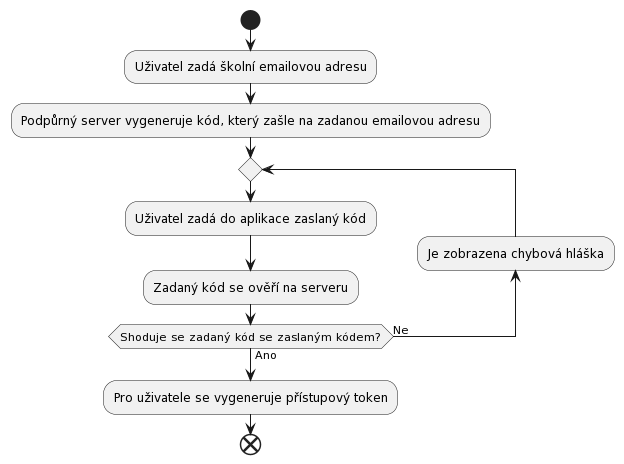
\includegraphics[width=\textwidth]{img/autentikace.png}
    \caption{Vývojový diagram přihlášení uživatele (vlastní zpracování)}
    \label{fig:autentikace}
\end{figure}
\imgsource{
@startuml
start
:Uživatel zadá školní emailovou adresu;
:Podpůrný server vygeneruje kód, který zašle na zadanou emailovou adresu;
repeat 
    :Uživatel zadá do aplikace zaslaný kód;
    :Zadaný kód se ověří na serveru;
backward :Je zobrazena chybová hláška;
repeat while (Shoduje se zadaný kód se zaslaným kódem?) is (Ne) not (Ano)
:Pro uživatele se vygeneruje přístupový token;
end
@enduml
}

\begin{figure}[htbp!]\centering
    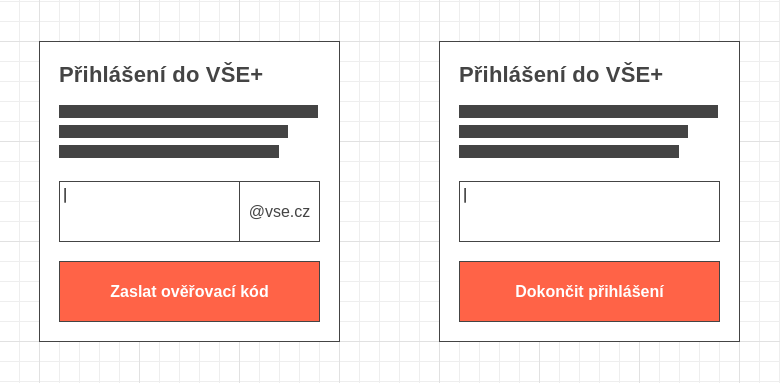
\includegraphics[width=\textwidth]{img/wireframe-autentikace.png}
    \caption{Návrh grafického rozhraní přihlášení uživatele (vlastní zpracování)}
    \label{fig:autentikace-wireframe}
\end{figure}

\section{Zobrazení náhledu rozvrhu při registracích předmětů}

První funkcionalitou, kterou webové rozšíření do informačního systému InSIS přidává, je zobrazení náhledu rozvrhu a detekce kolizí se zapsanými hodinami při registraci rozvrhových akcí. V~uživatelském rozhraní pro registraci rozvrhových akcí nejsou v~informačním systému InSIS zobrazené již zaregistrované rozvrhové akce a je tedy velice obtížné si efektivně sestavovat rozvrh. Většina dotazovaných studentů tento nedostatek řeší tak, že si registrují předměty za pomoci kombinace 2 prohlížečových oken, kdy v~jednom okně prohlížeče mají otevřený rozvrh a v~druhém okně prohlížeče mají otevřené registrace předmětů. Kolize studenti hledají manuálně, často až pomocí vizuální kontroly po registraci rozvrhové akce.

Efektivitu uživatelů systému InSIS při registraci rozvrhových akcí je možné zlepšit zobrazením náhledu rozvrhu s~již zaregistrovanými rozvrhovými akcemi vedle seznamu dostupných rozvrhových akcí pro předmět, který si uživatel aktuálně zapisuje. Další zlepšení efektivity pak poskytuje automatická detekce kolizí v~rozvrhu a vizuální odlišení hodin s~kolizí ve výběru dostupných rozvrhových akcí. Toto odlišení může být implementováno například jako zvýšení průhlednosti řádků v~tabulce. 

Při zápisu rozvrhových akcí při registracích předmětů je celý obsah stránky zarovnaný na levou stranu obrazovky a při zápisu u~většiny rozvrhových akcí formulář pro výběr dne a času nezabírá ani polovinu dostupného místa na obrazovce. Proto je vhodné implementovaný náhled rozvrhu s~již zaregistrovanými rozvrhovými akcemi umístit do pravé části obrazovky.

Celý funkční proces pro náhled rozvrhu při registraci rozvrhových akcí popisuje diagram zobrazený na obrázku \ref{fig:wireframe-timetable-preview}.

\begin{figure}[htbp!]\centering
    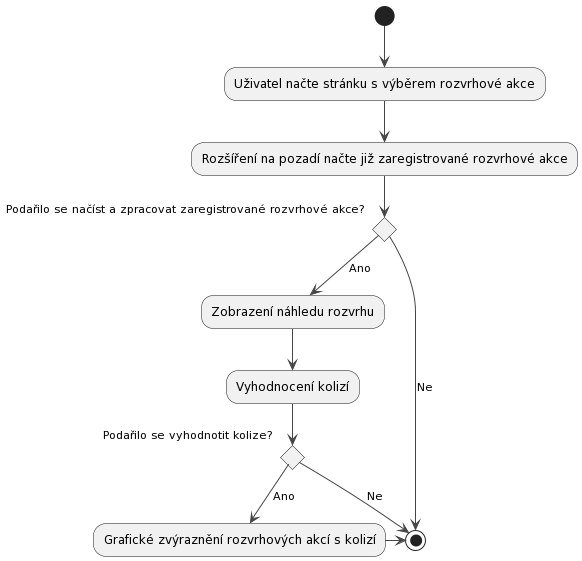
\includegraphics[width=\textwidth]{img/flow-timetable-preview.png}
    \caption{Vývojový diagram popisující funkcionalitu náhledy rozvrhů (vlastní zpracování)}
    \label{fig:wireframe-timetable-preview}
\end{figure}
\imgsource{
    @startuml
    (*) --> "Uživatel načte stránku s~výběrem rozvrhové akce"
    
    --> "Rozšíření na pozadí načte již zaregistrované rozvrhové akce"
    
    if "Podařilo se načíst a zpracovat zaregistrované rozvrhové akce?" then
      -->[Ano] "Zobrazení náhledu rozvrhu"
      --> "Vyhodnocení kolizí"
      if "Podařilo se vyhodnotit kolize?" then
        -->[Ano] "Grafické zvýraznění rozvrhových akcí s~kolizí"
        -right-> (*)
      else
         -right->[Ne] (*)
      endif
    else
      -right-->[Ne](*)
    endif
    @enduml
}

\section{Připomenutí odevzdáváren a export do externího kalendáře}\label{sec:pripomenuti-odevzdavaren}

Nedílnou součástí školního informačního systému InSIS je modul odevzdávárny. Tento modul slouží pro nahrávání a odevzdávání souborů a je nejčastěji využíván vyučujícími jako prostředek pro sběr vypracovaných domácích úkolů a seminárních prací. 

Jedním z~vypozorovaných nedostatků je absence možnosti si na odevzdávárnu nechat zaslat upozornění. Informační systém InSIS podobnou funkcionalitu u~některých jiných modulů nabízí. Příkladem může být funkce hlídací pes při přihlašování se na termíny zkoušek, pomoíc které si student může nechat zaslat oznámení na email v~případě, že se uvolní místo na vybraném termínu.

Tento nedostatek umocňuje skutečnost, že řada vyučujících vypisuje odevzdávárny pro celý semestr již během prvního týdne a je pak častým problémem, že student na některé z~pozdějších odevzdáváren zapomene, jelikož datum vypsání a datum uzavření mohou být od sebe i v~řádech několika měsíců.

Dalším potencionálním zlepšením práce uživatelů s~odevzdávárnami je možnost exportu a synchronizace datumů uzavření s~kalendářem. Podobně jako u~připomenutí, tato funkcionalita je dostupná v~několika jiných modulech informačního systému InSIS. Jedním z~příkladů může být opět modul pro přihlašování na termíny zkoušek, který umožňuje synchronizaci časů zkoušek s~kalendářem.

\subsection{Návrh rozložení prvků na stránce}

Z~analýzy grafického rozložení modulu pro odevzdávárny, že adekvátním řešením integrace uživatelského rozhraní pro připomínání odevzdáváren a export do externího kalendáře bude využití prázdného místa na pravé straně obrazovky rozšířením tabulky s~otevřenými odevzdávárnami o~2 nové sloupce.

Rozšířené nastavení připomenutí pro konkrétní odevzdávárnu bude implementováno v~podobě dialogového okna, které se otevře až po kliknutí na ikonu v~rozšířené tabulce. Tímto způsobem je možné schovat komplexní uživatelské rozhraní pro výběr časů a správu připomenutí až do chvíle, kdy je to pro uživatele systému přínosné a relevantní. 

\subsection{Export do kalendáře}

Podnět pro implementaci exportu času a předmětu odevzdáváren do externího kalendáře přišel od jednoho ze studentů, který stejně jako část dalších studentů na Vysoké škole ekonomické v~Praze, využívá synchronizaci rozvrhu se školním kalendářem Microsoft Outlook z~balíčku Microsoft Office 365.

Tato synchronizace se školním kalendářem podporuje kromě přímé synchronizace rozvrhových akcí v~rámci týdne i propisování datumů a časů zkoušek, na které je student přihlášen. Jednou z~informací, která v~tomto exportovaném kalendáři chybí jsou datumy a časy uzavření vypsaných odevzdáváren.

Po vyhodnocení dotazníkového šetření s~celkovým počtem 31 respondentů byly jako podporované externí kalendáře s~největším počtem respondentů zvoleny produkty Google Calendar a Microsoft Outlook.

\section{Vylepšený rozvrh}\label{sec:vylepseny-rozvrh}

Poslední z~navržených funkcionalit je vylepšená verze rozvrhu. Tato vylepšená verze se od původní verze liší jak po grafické, tak po funkční stránce. Nejzásadnějším rozdílem je integrace konceptu přepínání mezi jednotlivými výukovými týdny v~rámci rozvrhu. Původní implementace rozvrhu poskutovaná informačním systémem InSIS zobrazuje pouze statický rozvrh, který není závislý na aktuálně probíhajícím výukovém týdnu.

\subsection{Vylepšený vzhled rozvrhu}

Jelikož v~rámci implementace bude docházet k~sestavování nové DOM stromové reprezentace pro zobrazení komponent tvořících zobrazení rozvrhu, naskytuje se možnost jako součást  implementace vylepšit grafickou stránku rozvrhu. 

Pro vylepšenou verzi rozvrhu byla zvolena nová paleta barev, bylo změněno rozložení dílčích informací zobrazených v~buňkách reprezentujících rozvrhové akce a u~každé rozvrhové akce byl dále přidán explicitní čas začátku a konce. Poslední změnou je úprava mezer vně kontejneru pro zobrazení informací a úprava typografických vlastností textu pro zajištění lepší čitelnosti a zjednodušení orientace v~rozvrhu.

\subsection{Přepínání mezi týdny a zpracování rozvrhových výjimek}

Klíčovou změnou ve vylepšené verzi rozvrhu je práce s~jednotlivými výukovými týdny. To zahrnuje zobrazení aktuálního týdne v~záhlaví rozvrhu společně s~uživatelským rozhraním pro přepínání mezi týdny. Dále oproti původní implementaci rozvrhu probíhá navíc zpracování výjimek v~rozvrhových akcích, které jsou tvořeny zejména volnými dny, ve kterých výuka odpadá a dny, ve kterých probíhají blokových akcí. Pokud v~konkrétním týdnu rozvrhová akce neprobíhá, je rozvrhová akce v~rozvrhu graficky odlišena. Toto grafické odlišení poskytuje uživateli zrychlenou zpětnou vazbu oproti původní číselné poznámce pod rozvrhem, kterou je možné snadno přehlédnout.

Během zpracování poznámek v~rozvrhu dochází k~detekci začátku a konce výukového období, které je následně v~uživatelském rozhraní pro přepínání týdnů využito pro zobrazení pořadového čísla týdne, a jestli je tento týden součástí výukového období.

\subsection{Zobrazení aktuálního času v~rozvrhu}

Další přidanou funkcionalitou do zobrazení rozvrhových akcí je vyznačení aktuálního času přímo v~rozvrhu. Cílem této funkcionality je podobně jako u~zpracování výjimek rozvrhových akcí zlepšit zpětnou vazbu pro uživatele informačního systému, protože vyznačení aktuálního času v~rozvrhu zlepšuje navigaci a snižuje čas pro nalezení aktuálně probíhající hodiny. 

\subsection{Možnost přidání poznámek ke konkrétním hodinám}

Poslední přidanou funkcionalitou, která rozšiřuje funkce rozvrhu je možnost přidávání poznámek ke konkrétním hodinám. To je užitečné zejména pro označení naplánovaných průběžných testů, domácích úkolů nebo prezentací. 

Z~konzultací s~ostatními studenty vyplynulo, že značná část dotazovaných studentů sdílí workflow pro přípravu na nadcházející týden s~autorem práce. Tento workflow spočívá v~párování hodin v~rozvrhu s~externě poznamenanými testy, úkoly a prezentacemi. Nejčastějším prostředkem pro poznámky k~hodinám je externí aplikace pro psaní textových poznámek, správy úkolů\footnote{Například aplikace Google Keep nebo Microsoft To Do} nebo kalendář.

Správa poznámek přímo v~rozvrhu umožňuje zefektivnění přípravy na hodiny, protože spojuje všechny potřebné informace do jednoho uživatelského rozhraní bez nutnosti přepínání mezi aplikacemi.

Z~analýzy dotazníkového šetření, kterou popisuje kapitola \ref{chap:zpetna-vazba}, vyplynulo, že tento předpoklad očekávané práce studentů s~rozvrhem byl mylný a přidanou funkcionalitu poznámek v~rozvrhu využívá pouze menšina uživatelů rozšíření.

\chapter{Volba technologií a návrh architektury}\label{chap:volba-technologii}

Tato kapitola stručně představuje a srovnává některé z~dostupných technologií, které je možné použít pro implementaci obou částí softwarového řešení. 

\section{Volba technologie pro webové rozšíření}

Pro webové rozšíření bylo potřeba zvolit technologii, která umožňuje kompilaci nebo transpilaci do jazyka JavaScript, protože to je jediný programovací jazyk, který je podporován v~běhovém prostředí webových prohlížečů.

Transpilace je proces, při kterém dochází k~překladu zdrojových kódů z~původního programovacího jazyka do syntetizovaného kódu v~cílovém jazyce \cite{fowler_transparent_2013}. 

Je poměrně časté, že v~procesu transpilace je zdrojový a cílový jazyk stejný programovací jazyk, ale jedná se o~jinou verzi tohoto jazyka. Typickým důvodem pro takovou transpilaci je zachování zpětné kompatibility se staršími verzemi daného programovacího jazyka. Pomocí této transpilace je možné používat například moderní syntaxi a jazykové konstrukce, které byly přidané až v~novější verzi tohoto programovacího jazyka, bez dopadu na míru podpory těchto přidaných konstrukcí v~běhovém prostředí.

\subsection{Výčet některých z~dostupných technologií}

Pro implementaci rozšíření do webového prohlížeče se naskytuje několik programovacích jazyků, které splňují vymezené požadavky na kompatibilitu s~běhovým prostředím internetových prohlížečů:

\begin{itemize}
    \item JavaScript
    \item TypeScript
    \item Kotlin s~nadstavbou Kotlin/JS
    \item Ostatní programovací jazyky s~podporou transpilace do jazyka JavaScript
\end{itemize}

Pro každý z~těchto programovacích jazyků existuje řada pro a proti, které je potřeba při výběru zvážit. V~následujících odstavcích je stručně představena každá z~variant společně s~výhodami a nevýhodami daného programovacího jazyka.

\subsubsection{JavaScript}

 Programovací jazyk JavaScript je implementací specifikace jazyka ECMAScript a jedná se v~dnešní době o~jeden z~nejrozšířenějších jazyků vůbec. Bezesporu největší výhodou tohoto jazyka je, že je přímo podporovaný v~běhovém prostředí webových prohlížečích, a není tedy potřeba zavádět žádný další krok pro sestavení kódu rozšíření \cite[kap. 1]{flanagan_javascript_2020}. 
 
 Nevýhodou programovacího jazyka JavaScript je, že se jedná o~dynamicky typovaný programovací jazyk. To znamená, že datové typy proměnných se vyhodnocují až za běhu programu, a je tedy mnohem jednodušší udělat při psaní programu chybu v~porovnání s~programovacími jazyky, které jsou staticky typované. Staticky typované programovací jazyky jsou takové jazyky, u~kterých je datový typ všech proměnných znám již při překladu programu \cite[kap. 3.1]{flanagan_javascript_2020}.

\subsubsection{TypeScript}

Programovací jazyk TypeScript je z~pohledu syntaxe striktní nadmnožinou programovacího jazyka JavaScript. 
To implikuje, že jakýkoliv syntakticky validní program napsaný v~jazyce JavaScript je zároveň syntakticky validním programem v~jazyce TypeScript. Zmíněná implikace však neplatí opačným směrem, protože TypeScript rozšiřuje JavaScript o~novou syntaxi a jazykové konstrukce, které nejsou v~jazyce JavaScript nativně podporovány \cite{cherny_programming_2019}

Nejzásadnější přidanou hodnotou jazyka TypeScript, jak již název naznačuje, je podpora pro typový systém, který tento programovací jazyk zařazuje mezi staticky typované programovací jazyky, protože všechny datové typy jsou předem známy již při překladu programu. 

Ve výpisech \ref{code:javascript-bad} a \ref{code:typescript-good} je vidět porovnání programovacích jazyků JavaScript a Typescript společně s~nastíněním výhod, které přináší využití programovacího jazyka TypeScript.

\begin{lstlisting}[label={code:javascript-bad}, caption={Ukázka kódu s~neplatným typem parametru v~jazyce JavaScript (vlastní zpracování)}]
// JavaScript
function format(price) {
    return price.toFixed(2);
}

format(2.134); // -> '2.13'
format("2.134"); // Způsobí chybu až při spuštění programu
// Uncaught TypeError: price.toFixed is not a function
\end{lstlisting}

\clearpage
\begin{lstlisting}[label={code:typescript-good}, caption={Ukázka kódu s~neplatným typem parametru v~jazyce TypeScript (vlastní zpracování)}]
// TypeScript
function format(price: number): string {
    return price.toFixed(2);
}

format(2.134); // -> '2.13'
format("2.134"); // Způsobí chybu při kompilaci, ještě před spuštěním
// Argument of type 'string' is not assignable to parameter of type 'number'.
\end{lstlisting}

Výhodou jazyka TypeScript je interoperabilita s~jazykem JavaScript, která umožňuje z~jazyka TypeScript využívat softwarové knihovny napsané v~jazyce JavaScript, včetně již zmíněného API poskytovaného běhovým prostředím webového prohlížeče. Pro tyto knihovny a API často existují typové definice, což jsou speciální soubory, které obsahují externí deklaraci typů pro existující JavaScript knihovny. Tyto typové definice je možné nainstalovat spolu s~ostatními závislostmi programu. Například typové definice pro API běhového prostředí Node.js jsou dostupné v~podobě NPM (Node Package Manager) balíčku \verb|@types/node| \cite[kap. 2]{cherny_programming_2019}.

Nevýhodou jazyka TypeScript je, že webové prohlížeče neumí na rozdíl od jazyka JavaScript kód v~jazyce TypeScript nativně interpretovat a proto je nutné před spuštěním celý program transpilovat do jazyka JavaScript, který odstraní typové definice a ostatní přidané syntaktické a jazykové konstrukce, které nejsou součástí specifikace ECMAScript. 

\subsubsection{Kotlin/JS}\label{sec:kotlin}

Kotlin je programovací jazyk vyvinutý společností JetBrains s.r.o., která se specializuje v~oblasti vývoje programovacích nástrojů a vývojových prostředí. Jedná se o~programovací jazyk, který je možné zkompilovat do několika cílových výstupních formátů. Dominantním cílem kompilace pro jazyk Kotlin je JVM bytecode, což je nativní kód pro prostředí Java Virtual Machine. Programovací jazyk Kotlin umožňuje mimo jiné i kompilaci do nativního strojového kódu pomocí Kotlin native s~vazbami na nástroj LVVM (Low Level Virtual Machine) a transpilaci do jazyka JavaScript pomocí platformy Kotlin/JS.

Stejně jako u~programovacího jazyka TypeScript, programovací jazyk Kotlin nabízí interoperabilitu s~již existujícími JavaScript knihovnami, která je zprostředkovaná pomocí typových deklarací a anotací. 
U~JavaScript knihoven, které se distribují společně s~typovými definicemi jazyka TypeScript je možné využít nástroj Dukat, který automaticky konvertuje typové definice jazyka TypeScript do typových definic jazyka Kotlin. Alternativou je manuální definice těchto typových definic.

V~jazyce Kotlin k~tomuto účelu slouží klíčové slovo \code{external}, které definuje objekty, funkce, třídy a další entity z~externích knihoven. Výpisy \ref{code:kotlin-js-javascript} a \ref{code:kotlin-js-typedefs} zobrazují implementaci jednoduché softwarové knihovny v~programovacím jazyce JavaScript a k~ní přidružené typové definice v~programovacím jazyce Kotlin.

\begin{lstlisting}[label={code:kotlin-js-javascript}, caption={Jednoduchá JavaScript knihovna pro demonstraci typových definic v~jazyce Kotlin (vlastní zpracování)}]
// library.js
const square = (x) => x * x;

function add(x, y) {
    return x + y;
}

class Node {
    constructor(x) {
        this.x = x; 
    }
}
\end{lstlisting}

\begin{lstlisting}[label={code:kotlin-js-typedefs}, caption={Typové definice v~jazyce Kotlin pro externí JavaScript knihovnu (vlastní zpracování)}]
// typedef.kt
external val square: (Int) => Int
external fun add(x: Int, y: Int): Int
external class Node(val x: Int)
\end{lstlisting}

Kotlin/JS přináší několik výhod. První, subjektivní výhodou pro tento konkrétní projekt je, že s~tímto programovacím jazykem má autor již dlouholetou zkušenost. Mezi další, již více objektivní, výhody patří mimo jiné typový systém jazyka Kotlin, který přináší zlepšení oproti typovému systému, který implementuje programovací jazyk TypeScript. Příkladem zlepšení může být rozlišení datových typů pro celočíselná a desetinná čísla v~různých bitových velikostech. Další z~výhod je rozsáhlejší standardní knihovna programovacího jazyka Kotlin, kterou je možné přímo v~rámci programu využívat. 

Potencionální výhodou by v~případě, že by tento programovací jazyk byl zvolen pro implementaci webového rozšíření, jsou již existující vazby a typové definice pro populární knihovnu React.js, které spravuje přímo firma JetBrains s.r.o., což zaručuje kvalitu typových definic a lepší komerční i nekomerční podporu než u~knihoven, které vyvíjí jeden člověk,  a to navíc často ve svém volném čase.

Hlavní nevýhodou použití jazyka Kotlin je náročný proces kompilace, který vyžaduje celou řadu externích nástrojů. Další nevýhodou tohoto programovacího jazyka je, že v~době psaní této práce neexistuje typová definice pro velice obsáhlé aplikační rozhraní webových prohlížečů, která by musela být nadefinována v~rámci projektu, což by bylo velice složité a časově náročné, protože prohlížeče pracují s~rozšířenou sadou objektů oproti běhovému prostředí pro aplikace webových stránek, pro které je Kotlin/JS primárně určen.

\subsubsection{Ostatní programovací jazyky s~podporou transpilace do jazyka JavaScript}

Existuje řada dalších programovacích jazyků, které podporují transpilaci do jazyka JavaScript. Jedná se například o programovací jazyky Scala, Clojure, PureScript, CofeeScript, Dart, ReasonML nebo Haxe.

Žádný z~těchto programovacích jazyků avšak nepřináší v~kontextu webových rozšíření zásadní výhody oproti již představeným programovacích jazykům a jedná se často pouze o~preferenci syntaxe daného jazyka.

\subsection{Zvolená technologie}

Po zvážení výhod a nevýhod zmíněných jazyků byl pro implementaci rozšíření zvolen programovací jazyk TypeScript, protože nabízí nejlepší kompromis mezi rychlostí vývoje a zárukami ohledně výsledného kódu. Sestavování transpilovaného výstupu v~jazyce JavaScript je v~případě využití programovacího jazyka TypeScript přímočaré a kompilátor pro překlad TypeScript kódu je možné spouštět velice často a kompilace menšího až středně velkého projektu se pohybuje v~nižších jednotkách sekund. 

Rychlost transpilace se pohybuje u~menších projektů maximálně v~jednotkách sekund, častěji spíše v~desítkách až stovkách milisekund. V~porovnání například se zmíněnou technologií Kotlin/JS jde o~výraznou redukci kompilačního času, protože transpilace z~jazyka Kotlin do jazyka JavaScript přes nástroj Gradle může trvat až několik minut, což se může velice negativně projevit na produktivitě při vývoji rozšíření.

\section{Volba technologie pro podpůrný webový server}

Pro podpůrný webový server se nabízí daleko širší spektrum technologií, ze kterých je možné pro implementaci programu vybírat. Tato diverzita je dána mimo jiné tím, že na podpůrný webový server není kladeno omezení na kompatibilitu s~konkrétním běhovým prostředím, jako je tomu u~rozšíření do webových prohlížečů. 

\subsection{Požadavky na zvolenou technologii}\label{sec:pozadavky-na-zvolenou-technologii}

Vybraný programovací jazyk a webový aplikační rámec musí podporovat následující požadavky na vestavěné funkcionality, aby bylo možné tento rámec pro implementaci podpůrného webového serveru použít:

\begin{itemize}
    \item Přijímání a odpovídání na přijaté HTTP požadavky,
    \item serializace a parsování formátu JSON pro přenos dat,
    \item komunikace s~databází, ve které jsou uložená data uživatelů,
    \item podpora pro autentikaci a autorizaci uživatelů s~využitím HTTP hlaviček,
    \item odesílání emailů pomocí vestavěného nebo externího SMTP serveru.
\end{itemize}

Tyto požadavky splňuje množství aplikačních rámců napříč širokou škálou programovacích jazyků. Toto spektrum technologií bylo zúženo na 4 konkrétní aplikační rámce, které budou popsány v~následujících podkapitolách.

\subsection{Představení dostupných technologií}

\subsubsection{Spring framework}\label{sec:spring-boot}

% https://spring.io/

Spring Framework a jeho nadstavba Spring Boot je aplikační rámec vyvinutý společností Pivotal v~roce 2004 \cite{risberg_spring_2004}. Společnost Pivotal je od roku 2019 součást společnosti VMware \cite{vmware_pivotal_acquisition_2019}. Jedná se o~open source aplikační rámec, který staví na technologii programovacího jazyka Java a je proto možné pro vývoj aplikací v~tomto aplikačním rámci použít libovolný programovací jazyk, který je kompatibilní s~běhovým prostředím Java Virtual Machine. Oficiálně podporovanými programovacími jazyky jsou Java, Kotlin a Groovy \cite{spring_framework}.

Spring nabízí řadu modulů, které je možné využít při programování aplikací. Tyto moduly jsou dostupné jako samostatné balíčky a je možné je specifikovat v~rámci závislostí v~nástroji pro sestavování balíčků jako je například Maven nebo Gradle. Tato modularita nabízí flexibilitu při vývoji aplikací, kdy nedochází ke stahování, kompilaci a exportu softwarových knihoven, které nejsou pro konkrétní aplikaci potřeba. Příkladem může být modul \code{spring-data}, který poskytuje sdílenou logiku a abstrakce pro načítání dat z~relačních a NoSQL databází. Pokud aplikace nepotřebuje ukládat data v~databázi a místo toho data získává například z~externího REST API, není potřeba tento modul do aplikace přidávat, čímž dojde k~redukci komplexity, času sestavení a spuštění aplikace a velikosti výsledného sestaveného balíčku \cite{spring_boot}.

Pro správu těchto modulů a vytváření nových projektů s~využitím aplikačního rámce Spring je možné použít webový nástroj Spring Initalizr, který je dostupný na následující URL adrese \url{https://start.spring.io} \cite{spring_boot}.

\begin{figure}[htbp!]\centering
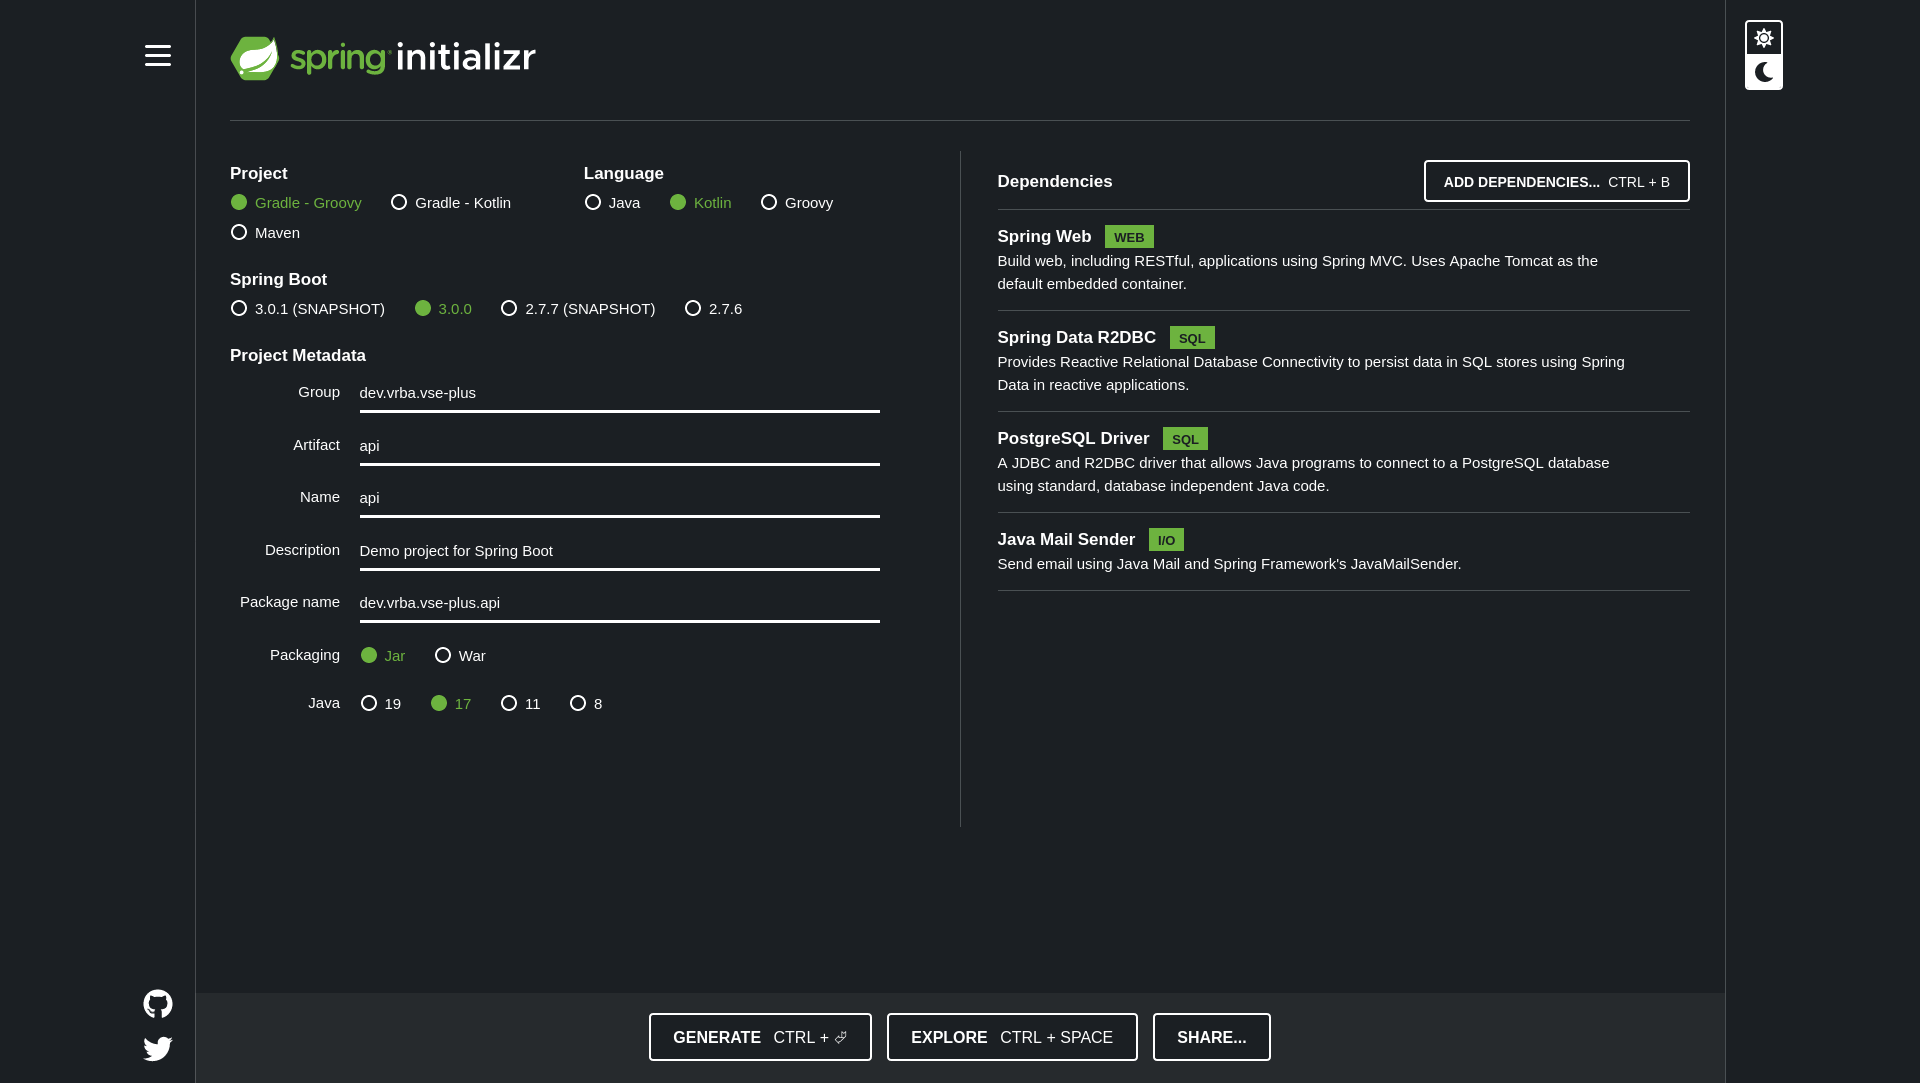
\includegraphics[width=\textwidth]{img/sprint-initializr.png}
\caption{Webové rozhraní nástroje Spring Initializr (vlastní zpracování)}
\label{obr1:SpringInitializr}
\end{figure}

Pro splnění požadavků kladených na funkcionalitu podpůrného serveru vytyčených v~kapitole \ref{sec:pozadavky-na-zvolenou-technologii} je možné použít následující moduly:

\begin{itemize}
    \item \verb|spring-web| pro příjímání a odpovědi na HTTP požadavky,
    \item \verb|spring-json| pro zpracování formátu JSON. Je součástí modulu \verb|spring-web|,
    \item \verb|spring-data| pro ukládání a načítání dat z~relační databáze,
    \item \verb|spring-security| pro autentikaci a autorizaci uživatelů,
    \item \verb|spring-mail| pro odesílání emailů pomocí externího SMTP serveru.
\end{itemize}

\subsubsection{ASP.NET}

ASP.NET je aplikační rámec pro vývoj webových aplikací pomocí technologie .NET vyvinutý společností Microsoft. Podobně jako u~aplikačního rámce Spring se jedná o~platformu, která není omezená pouze na vývoj webových aplikací. Jedná se například o~velice populární platformu vývoj desktopových aplikací pro operační systém Windows.

Aplikační rámec ASP.NET byl poprvé vydán společností Microsoft v~roce 2002 \cite{bekker_microsoft_2002} a jedná se o~zdaleka nejpopulárnější aplikační rámec pro programovací jazyky založené na běhovém prostředí CLR (Common Language Runtime), mezi které patří například programovací jazyk C\# nebo Visual Basic \cite{warren_clr_2022}.

Rámec ASP.NET poskytuje všechny potřebné moduly pro implementaci požadavků kladených na podpůrný webový server. Přímo aplikační rámec ASP.NET má zabudovanou podporu pro příjímání a odpovědi na HTTP požadavky a zpracování formátu JSON \cite{dotnet_web_2023}.

Pro podporu autentikace a autorizace uživatelů má ASP.NET připravenou sadu externích balíčků, které umožňují registrovat schémata pro autentikaci uživatelů a následně definovat přístupová pravidla pro autorizaci uživatelů \cite{dotnet_security_2022}.

\subsubsection{Laravel}

Laravel je webový aplikační rámec vyvinutý pro vývoj webových aplikací v~programovacím jazyce PHP. Programovací jazyk PHP je open source jazyk speciálně navržený pro tvorbu webových aplikací \cite{what_is_php}. Aplikační rámec Laravel poskytuje podporu pro časté požadavky na webové aplikace v~podobě externích balíčků pro práci s~databázovými systémy, autentikace a autorizace uživatelů, zasílání emailů, renderování šablon a další \cite{laravel}. 

Stejně jako předchozí dva zmíněné aplikační rámce, Laravel poskytuje formu abstrakce nad vymezenými funkcionalitami, což umožňuje rychlejší a jednodušší tvorbu aplikací, protože se o~konkrétní funkcionalitu stará přímo aplikační rámec a nikoliv programátor, který tento aplikační rámec využívá.

Jednou z~předností aplikačního rámce Laravel je vysoká rychlost a dynamika při vývoji webových aplikací a krátká zpětnovazební smyčka, což je dobré zejména pro vývoj prototypů výsledného produktu, které můžou být využity pro otestování business modelu a najití potencionálních míst pro zlepšení.

\subsection{Zvolená technologie}

Po zvážení výhod a nevýhod všech zmíněných technologií byl zvolen pro implementaci podpůrného webového serveru aplikační rámec Spring Boot ve spojení s~programovacím jazykem Kotlin, protože nejlépe odpovídal potřebám autora a protože s~programováním serverů v~této kombinaci programovacího jazyka a aplikačního rámce má autor již dlouholetou předchozí zkušenost. Programovací jazyk Kotlin byl zvolen mimo jiné i kvůli jeho výhodám oproti programovacímu jazyku Java, které byly zmíněny v~kapitole \ref{sec:kotlin}.
\chapter{Implementace webového serveru}\label{chap:server}

Pro zajištění infrastruktury pro funkcionality mimo samotný informační systém InSIS, jako je například ukládání uživatelských dat nebo rozesílání emailů s~připomenutím odevzdáváren je potřeba implementovat podpůrný webový server. 

\section{Konfigurace projektu}

Jako první byl vygenerován základ projektu pomocí nástroje Spring Initializr, který byl zmíněn v~kapitole \ref{sec:spring-boot}. Tento nástroj umožňuje konfiguraci projektu včetně jeho závislostí a stažení celého projektu jako archiv pro následnou extrakci.

Konfigurace projektu spočívá ve výběru build systému, výběru verze aplikačního rámce Spring Boot, nastavení metadat projektu, výběr verze cílového běhového prostředí jazyku Java a výběru závislostí a balíčků, které mají být v~projektu zahrnuty.

Jako build systém, tedy komplexní programový nástroj používaný pro správu závislostí a sestavování výsledného Java balíčku, je možné si vybrat mezi nástroji Apache Maven a Gradle. Pro Java projekty je časté využití nástroje Apache Maven, který je výchozí možností pro zakládání nového Spring projektu. Pro programovací jazyky Kotlin a Groovy je ale častější volbou nástroj Gradle, protože umožňuje definovat konfiguraci pomocí DSL (Domain Specific Language) přímo v~konkrétním programovacím jazyce. Kontrastně k~nástroji Gradle, v~nástroji Apache Maven probíhá konfigurace s~využitím značkovacího jazyka XML \cite{pom_reference}. Pro projekt byl tedy zvolen nástroj Gradle s~konfigurací pomocí DSL v~jazyce Kotlin.

Metadata projektu byly nastaveny podle používaných konvencí. Jako atribut group, tedy skupinu vlastnící projekt, byla nastavena invertovaná osobní doména autora \url{dev.vrba}. Použití invertované domény je často používaná konvence pro názvy balíčků a jmenných prostorů v~programovacích jazycích platformy Java Virtual Machine. Konvence spočívá v~přeskládání jednotlivých úrovní domény. Například pro doménu \url{java.fis.vse.cz} by odpovídal podle této konvence název \url{cz.vse.fis.java}. Jako název artefaktu byl zvolen \verb|vse-plus-api|. Jako název balíčku se podle konvencí často uvádí spojení skupiny a názvu artefaktu, tedy v~tomto případě \url{dev.vrba.vse-plus-api}. 

Tento identifikátor ale není v~programovacích jazycích Java a Kotlin validní název balíčku, protože názvy balíčku nesmí obsahovat pomlčky \cite{gosling_java_2022}. Z~tohoto důvodu byl název hlavního balíčku změněn na \url{dev.vrba.vseplus.api}. Jako verzi programovacího jazyka Java, do kterého se má projekt při sestavení zkompilovat byla zvolena verze Java 17, která byla v~době vytváření projektu nejnovější verzí programovacího jazyka Java, podporovaného v~aplikačním rámci. V~době psaní této práce je nejnovější verzí programovacího jazyka Java podporovanou v~aplikačním rámci Spring verze 19.

Jako závislosti pro projekt bylo z~nabídky modulů v~nástroji Spring Initializr zvoleno celkem 6 modulů:

\begin{itemize}
    \item \url{spring-data-r2dbc}: knihovna pro reaktivní práci s~databází,
    \item \url{spring-mail}: knihovna pro odesílání emailů,
    \item \url{spring-security}: knihovna pro autentikaci a autorizaci,
    \item \url{spring-thymeleaf}: knihovna pro vykreslování šablon,
    \item \url{spring-validation}: knihovna pro validaci formátu dat,
    \item \url{spring-webflux}: knihovna pro reaktivní obsluhu HTTP požadavků.
\end{itemize}

\section{Struktura projektu}

Celý projekt je členěn do balíčků podle typu komponent. To je jedním ze dvou hlavních přístupu při dělení softwarových balíčků v~projektech využívající aplikační rámec Spring. Druhým přístupem při dělení balíčků je dělení podle domény, se kterou kód v~daném balíčku pracuje. První přístup tedy seskupuje například servisní třídy do jednoho balíčku a kontrolery do druhého balíčku. Druhá metoda pak seskupuje do jednoho balíčku servisní třídy společně s~kontrolery, které se týkají například uživatelských účtů, do jednoho balíčku. Servisní třídy a kontrolery například pro připomenutí odevzdáváren pak do jiného balíčku. Ani jedna z~metod neposkytuje objektivní výhody nebo nevýhody oproti druhé a proto byla zvolina první z~uvedených metod čistě na základě autorovy osobní preference. 

V~kořenovém adresáři projektu se nachází konfigurační soubory pro build systém Gradle. Kromě hlavního konfiguračního souboru \code{build.gradle.kts}, který definuje závislosti a vlastnosti projektu se zde nachází i takzvané wrapper scripty. Tyto skripty slouží ke spouštění nástroje Gradle bez nutnosti předchozí instalace. První wrapper script s~názvem \code{gradlew.bat} je určen pro platformu Windows a druhý s~názvem \code{gradlew} je určen pro platformy Mac OS a Linux \cite[kap. 3.4]{muschko_gradle_2014}.

Vedle konfiguračních souborů pro nástroj Gradle se v~kořenovém adresáři nachází složka \code{src}, která obsahuje veškeré zdrojové kódy projektu. V~této složce se nachází 2 podsložky s~názvy \code{main} a \code{test}. Jak název složek napovídá, složka \code{main} obsahuje zdrojové aplikaci pro hlavní balíček a složka \code{test} obsahuje zdrojové kódy pro testy k~projektu. Ve složce \code{main} se pak nachází 2 typy souborů. Prvním typem jsou samotné zdrojové kódy v~jazyce Kotlin, které se nachází v~podsložce \code{kotlin} a druhým typem jsou konfigurační a statické soubory, které se nachází v~podsložce \code{resources}.

Pro návrh business logiky podpůrného webového serveru byla zvolena takzvaná layered architecture. Jedná se o~softwarovou architekturu, která vychází z~odděleních jednotlivých částí aplikace do vrstev, které spojují softwarové komponenty v~rámci vrstvy do jednoho funkčního celku \cite{richards_software_architecture_patterns_2015}.

\section{Datová vrstva aplikace}

Jednou ze základních vrstev aplikace je datová vrstva, která zajišťuje načítání a ukládání dat v~relační databázi.
Jako systém pro řízení báze dat byl zvolen open source nástroj PostgreSQL. Tento software byl vybrán primárně kvůli tomu, že se je možné tento systém řízení báze dat provozovat zdarma bez poplatků spojených s~licencí, jako je tomu například u~systému řízení báze dat společnosti Oracle. Tento systém řízení báze dat je dále jedním z~oficiálně podporovaných databázových systémů, se kterými dokáže pracovat aplikační rámec Spring a jeho modul Spring Data \cite{spring_data}.

\subsection{Návrh databázového schématu}

Návrhu databázového schématu předcházelo vymezení jednotlivých entit, které budou reprezentovány tabulkami v~relační databázi. Tyto entity představují datové domény, které se budou v~aplikační databázi ukládat.

\subsubsection{Seznam entit}

V~databázovém schématu je možné vymezit celkem 4 entity, se kterými se v~rámci aplikace pracuje.

\begin{itemize}
    \item Uživatelský účet -- tabulka \code{accounts},
    \item připomenutí odevzdáváren -- tabulka \code{submission\_reminders},
    \item poznámky v~kalendáři -- tabulka \code{timetable\_events},
    \item oznámení -- tabulka \code{notifications}.
\end{itemize}

Na obrázku \ref{fig:db-schema} je zobrazeno vyhotovené databázové schéma včetně relací mezi tabulkami, které reprezenutují definované entity. Kromě tabulek zobrazených v~rámci schématu obsahuje databáze ještě další 2 tabulky, jednu s~názvem \code{liquibase\_changelog} a druhou s~názvem \code{liquibase\_changelog\_lock}. Tyto 2 tabulky jsou spravované migračním nástrojem Liquibase, jehož využití je dále podrobněji popsáno v~kapitole \ref{chap:liquibase}.

\begin{figure}[htbp!]\centering
    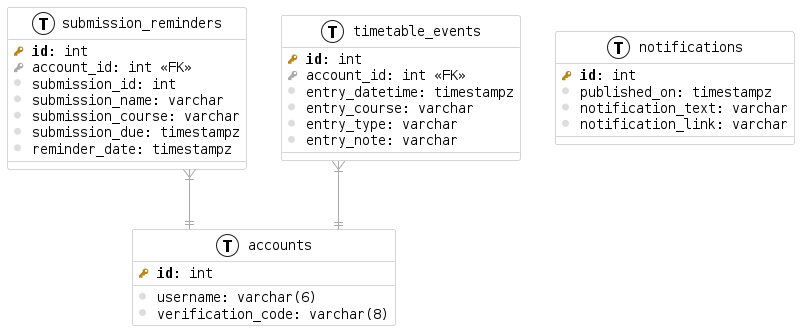
\includegraphics[width=\textwidth]{img/databazove-schema.png}
    \caption{Databázové schéma (vlastní zpracování)}\label{fig:db-schema}
\end{figure}
\imagesource{
@startuml
!define primary\_key(x) <b><color:#b8861b><&key></color> x</b>
!define foreign\_key(x) <color:#aaaaaa><&key></color> x
!define column(x) <color:#dddddd><&media-record></color> x

skinparam roundcorner 5
skinparam linetype ortho
skinparam defaultFontName Courier

skinparam class \{
    BackgroundColor white
    ArrowColor #aaaaaa
    BorderColor #aaaaaa
\}

entity accounts << (T,white) >> \{
  primary\_key( id ): int
  column( username ): varchar(6)
  column( verification\_code ): varchar(8)
\}

entity submission\_reminders << (T,white) >> \{
  primary\_key( id ): int
  foreign\_key( account\_id ): int <<FK>>
  column( submission\_id ): int
  column( submission\_name ): varchar
  column( submission\_course ): varchar
  column( submission\_due ): timestampz
  column( reminder\_date ): timestampz
\}

entity timetable\_events << (T,white) >> \{
  primary\_key( id ): int
  foreign\_key( account\_id ): int <<FK>>
  column( entry\_datetime ): timestampz
  column( entry\_course ): varchar
  column( entry\_type ): varchar
  column( entry\_note ): varchar
\}

entity notifications << (T,white) >> \{
  primary_key(id): int
  column(published\_on): timestampz
  column(notification\_text): varchar
  column(notification\_link): varchar
\}

submission\_reminders \}|--|| accounts
timetable\_events \}|--|| accounts
@enduml
}

\subsection{SQL migrace pomocí nástroje Liquibase}\label{chap:liquibase}

Pro jednodušší správu databázového schématu v~rámci aplikace byl zvolen nástroj Liquibase. Jedná se o~open source softwarové řešení pro správu verzí databázových schémat pomocí migrací definovaných v~jednom z~podporovaných datových formátů \cite{liquibase_inc_2023}.

Z~podporovaných formátů, mezi které mimo jiné patří formát JSON, XML, YAML a SQL, byl zvolen pro potřeby podpůrného webového serveru formát SQL. Ten umožňuje definovat databázové migrace přímo v~jazyce SQL rozšířeným o~speciální kontrolní struktury chování, které je možné definovat jako komentáře. Všechny databázové migrace se nachází v~souboru \code{/src/main/resources/changelog.sql}.


Ve výpise \ref{code:liquibase-changelog} se nachází 2 typy těchto speciálních komentářů, které slouží jako kontrolní struktury pro nástroj Liquibase. Prvním typem je komentář \code{-{}-liquibase formatted sql} na prvním řádku souboru. Tímto komentářem musí začínat všechny soubory, které se mají zpracovat nástrojem Liquibase. Jedná se především o~kontrolní mechanismus, který zajišťuje, aby nedošlo k~spouštění SQL souborů, které nejsou určeny pro zpracování nástrojem Liquibase a neobsahují komentáře pro kontroly a definice migrací. Druhým typem speciálního komentáře jsou definice jednotlivých migrací. Každá migrace je definována pomocí speciálního komentáře \code{-{}-changeset}, který je následován dvojicí argumentů spojených dvojtečkou. Prvním argumentem je autor migrace a druhým je unikátní identifikátor označující danou migraci \cite{liquibase_inc_sql_changelog}.

\subsection{Definice doménových tříd a repozitářů}

Modul Spring Data aplikačního rámce Spring umožňuje deklarativně mapovat data z~databázových tabulek na atributy doménových tříd za pomocí anotací. Přikladem může být doménová třída \code{TimetableEvent}. Obsah souboru, ve kterém je tato třída definována je možné vidět ve výpise \ref{code:timetable-event-domain-class}. Mapování třídy na tabulku je realizováno pomocí anotace \code{@Table}, která jako parametr očekává název tabulky ze které se mají mapovat hodnoty. Další anotací, kterou modul Spring Data využívá pro mapování dat je anotace \code{@Id}, která indikuje, že anotovaný atribut odpovídá primárnímu klíči v~mapované tabulce. Takto anotovaný atribut musí být v~každé doménové třídě právě jeden. Tato anotace slouží mimo jiné i pro cachování a recyklaci vytvořených instancí, správy namapovaných entit a optimalizaci vygenerovaných databázových dotazů. Poslední anotací, které se v~rámci zmíněné doménové třídy využívá pro definici mapování, je anotace \code{@Column}. Tato anotace očekává jako parametr název sloupce, který v~databázové tabulce odpovídá anotovanému atributu definovaném v~doménové třídě. Konverze datových typů probíhá automaticky a je zajištěna ovladačem pro konkrétní systém řízení báze dat.

Pro načítání a ukládání dat z~tabulek pomocí doménových tříd slouží takzvané repozitáře. Při použití tradičního způsobu načítání dat z~relačních databází v~programovacím jazyce Java je zapotřebí ručně psát databázové SQL dotazy a zpracovávat výsledky dotazu pomocí tříd a rozhraní z~balíčku \code{java.sql}. Tento přístup je velice pracný a náchylný na chyby, které můžou nastat například v~podobě nevalidních SQL dotazů, nesprávné implementace mapování a konverze datových typů po načtení dat z~databáze nebo v~podobě chyb souvisejících s~narušením referenční integrity. 

Aplikační rámec Spring a modul Spring Data umožňuje tento tradiční přístup, který by bylo možné označit za spíše imperativní, nahradit deklarativní definicí repozitářů, které se starají o~načítání, cachování a ukládání dat pro konkrétní doménovou třídu a tedy posléze namapovanou databázovou tabulku. Nespornou výhodou repozitářů je jednoduchost jejich definice a použití. Repozitář lze definovat jako rozhraní označené anotací \code{@Repository}. Spring Data automaticky při vytváření aplikačního kontejneru vytvoří a zaregistruje instanci anonymní třídy, která implementuje definované rozhraní. Tuto instanci je možné následně z~aplikačního kontejneru získat pomocí dependency injection. Spring Data automaticky derivuje SQL dotazy z~názvu metod podle konvencí definovaných v~referenční dokumentaci tohoto modulu. Spring Data poskytuje řadu již definovaných generických rozhraní pro repozitáře, ze kterých je možné pro konkrétní repozitář zdědit často využívané definice metod. Příkladem může být generické rozhraní \code{CoroutineCrudRepository<T, ID>}, které obsahuje sadu definovaných CRUD (Create, Read, Update, Delete) metod jako je například \code{findById(id: ID): T}, která podle jmenné konvence odpovídá SQL dotazu \code{SELECT * FROM :table WHERE id = :id}. Například metoda \code{findByIdAndAccount} definovaná na repozitáři \code{TimetableEventsRepository} vypsaném ve výpise \ref{code:timetable-events-repository} odpovídá podle jmenné konvence SQL dotazu \code{SELECT * FROM timetable\_events WHERE id = :id AND account\_id = :account} ve kterém se za parametry \code{:id} a \code{:account} dosadí hodnoty předané při volání této metody \cite{spring_data}.

\section{Vrstva pro zajištění business logiky}

\subsection{Definice opakujících se událostí pro rozesílání upozornění}

Opakující se události je možné v~rámci aplikačního rámce Spring definovat pomocí metod s~anotací \code{@Scheduled}. Tato anotace přijímá kombinaci parametrů, které umožňují flexibilně sestavovat časové intervaly, ve kterých se má anotovaná metoda volat. Toho využívá třída \code{SendSubmissionRemindersNotificationsTask}, která obsahuje metodu \code{run}, kterou je možné vidět ve výpise \ref{code:send-submission-reminders-notifications-task}, která se spouští každých 5 minut. 

Tato metoda nejprve provede kontrolu, že aplikace není spuštěná v~testovacím prostředí a následně zavolá metodu \code{sendPendingSubmissionRemindersNotifications} na injektované instanci třídy \code{SubmissionRemindersService}.

\begin{lstlisting}[label={code:send-submission-reminders-notifications-task}, caption={Definice periodicky spouštěné metody run}]
@Scheduled(
    fixedRate = 5,
    timeUnit = TimeUnit.MINUTES
)
fun run(): Unit = runBlocking {
    // Do not run this task during tests
    if (!environment.acceptsProfiles(Profiles.of("test"))) {
        service.sendPendingSubmissionRemindersNotifications()
    }
}
\end{lstlisting}

\section{Prezentační vrstva}

Prezenční vrstva slouží pro komunikaci s~klienty API. To zahrnuje mimo jiné přijímání HTTP požadavků, validaci formátu a obsahu dat požadavku nebo odesílání HTTP odpovědí. Prezentační vrstva je tvořena ze dvou typů komponent, kontrolerů a rozhraní pro přenos a validaci dat.

\subsection{Definice tříd kontrolerů}

Kontrolery jsou speciálním typem tříd anotovaných pomocí anotace \code{@Controller} nebo specializovaných variant jako například \code{RestController}, které se starají o~odbavování HTTP požadavků. Každému HTTP endpointu, který příjimá požadavky odpovídá právě jedna metoda na kontroleru, která je označena anotací \code{RequestMapping} nebo některou z~jejich specializovaných variant. Tyto varianty jsou vázány na konkrétní HTTP metody a příkladem těchto specializovaných variant může být například anotace \code{@GetMapping}, která odpovídá na HTTP požadavky využívající metodu \code{GET} \cite[kap. 1.3.1]{walls_spring_2019}.

Příkladem kompletní definice a implementace kontroleru je třída \code{AccountsController}, kterou je možné vidět ve výpise \ref{code:accounts-controller}. Aplikační rámec Spring automaticky registruje třídy anotované pomocí \code{@RestController}, protože tato anotace dědí logiku z~anotace \code{@Component}, která způsobí vytvoření nové instance v~rámci aplikačního kontejneru \cite[kap. 11.1.2]{walls_spring_2019}.

Argument anotace \code{@RequestMapping} definuje část URL adresy, která je společná pro všechny metody bez vazby na konkrétní HTTP metodu. Metoda \code{createAccount}, která je anotovaná pomocí anotace \code{@PostMapping} s~parametrem \code{"/create"} bude tedy dostupná pomocí HTTP metody POST na URL adrese \code{/api/v1/account/create}. Druhá metoda \code{verifyAcocunt}, která je anotovaná pomocí anotace \code{@PostMapping} s~parametrem \code{"/verify"} bude dostupná obdobně jako metoda \code{createAccount} pomocí HTTP metody POST, ale tentokrát na adrese \code{/api/v1/account/verify}.

Tyto metody, které slouží pro obsluhu HTTP požadavků mají jako návratový typ generickou třídu \code{ResponseEntity<T>}. Instance této třídy aplikační rámec Spring následně převádí na HTTP odpovědi, které odešle klientovi. Tento datový typ obsahuje informace o~stavovém kódu, HTTP hlavičkách včetně hlavičky \code{Content-Type} a obsahu těla HTTP požadavku, jehož struktura odpovídá generickému typu \code{T} a který je následně serializován do formátu JSON. Tato serializace je důsledek použití anotace \code{RestController}, která oproti obecné anotaci \code{Controller} implikuje, že všechny výstupní hodnoty volání obslužných metod mají být serializovány a odeslány s~patřičnou hlavičkou \code{Content-Type}, jejíž hodnota je automaticky nastavena na hodnotu \code{application/json}.

\subsection{Definice tříd pro přenos dat}

Pro jasné vymezení datových typů reprezentující požadavky, které aplikace v~metodách kontrolerů přijímá, se využívají takzvané DTO (Data Transfer Object) třídy. Tento typ tříd se používá pro definici struktury požadavku nebo odpovědi společně s~validačními pravidly, které aplikační rámec Spring před zavoláním metody kontroleru validuje. Jednou z~takových tříd je například třída \code{CreateAccountRequest}, jejíž definici je možné vidět ve výpise \ref{code:create-account-request}, a kterou jako vstupní parametr očekává již zmíněná metoda \code{createAccount}. Tento parametr je anotovaný pomocí anotace \code{@RequestBody}, která dává aplikačnímu rámci Spring instrukci, že se mají hodnoty definované v~této třídě načíst z~těla HTTP požadavku, a dále pomocí anotace \code{@Valid}, která implikuje validaci požadavku pomocí pravidel definovaných na jednotlivých atributech třídy \code{CreateAccountRequest}.

Třída \code{CreateAccountRequest} obsahuje jediný atribut s~názvem \code{username}, na kterém jsou pomocí anotací z~balíčku \url{jakarta.validation.contraints} definované 3 pravidla, které se musí před voláním zvalidovat. Anotace \code{@NotBlank} určuje, že tento parametr nesmí v~požadavku chybět a že se nemůže jednat o~prázdný textový řetězec nebo o~textový řetězec, který je tvořený pouze z~netisknutelných znaků. Dále anotace \code{@Size} definuje pomocí parametrů \code{min} a \code{max} minimální a maximální délku textového řetězce tohoto atributu. Poslední anotací, která definuje validační pravidla pro atribut \code{username} je anotace \code{@Pattern}, která pomocí parametru \code{regexp} definuje regulární výraz, který se musí shodovat s~hodnotou v~atributu \cite[kap 2.3]{walls_spring_2019}. Tento konkrétní regulární výraz odpovídá formátu emailových adres přidělovaných studentům na Vysoké škole ekonomické v~Praze. Ve výpise je možné si všimnout, že všechny takto aplikované anotace začínají výrazem \code{field:}. Tato syntaxe v~jazyce Kotlin udává, na kterou z~částí vygenerovaného JVM kódu se má anotace aplikovat. V~případě \code{field} se anotace umístí na vygenerovanou statickou instanční proměnnou v~rámci syntetizované třídy \cite{ebel_mastering_2019}.

\section{Testování}\label{sec:testovani}

Testování je proces pro zajištění kvality vyvíjeného softwarového řešení. 

Testování se dělí na dvě hlavní části. Prvním typem je uživatelské testování, které se často označuje také jako manuální testování. V~tomto typu testování probíhá kontrola implementace pomocí ručního spouštění funkcionalit dle předem stanovených scénářů. Druhým typem je strojové testování, kdy testování probíhá pomocí spouštění testovacího kódu, který ověřuje správnou funkčnost testovaného kódu. Oba typy testování mají řadu výhod a nevýhod oproti druhému typu. 

Výhodou uživatelského testování je lidský faktor, který je v~procesu zahrnut. Tento lidský faktor umožňuje detekovat řádu kódovacích chyb, které nejsou možné pomocí strojových testů odhalit. Další výhodou manuálního testování je, že testovaný scénář přímo odpovídá zkušenosti uživatele koncového softwarového produktu a testování často probíhá na reálných zařízeních, které se mohou chovat odlišně, pokud se jedná o~simulátor. Uživatelské testování se často využívá při testování UI a UX aspektů softwarového řešení. Největší nevýhodou manuálního testování oproti strojovému je jeho časová a finanční náročnost společně s~velice omezenou možností replikace. 

Strojové testy je možné spouštět paralelně, zatímco tester musí uživatelské testy provádět sekvenčně. Kromě rychlosti spouštění testů v~případě strojového testování je výhodou snadná replikace. Sadu strojových testů je možné bez větších nákladů spouštět iterativně po každé změně a je možné takto kontinuálně ověřovat korektnost implementace. Oproti tomu, v~případě uživatelského testování je potřeba předat kód s~testovacím prostředím testerovi a a počkat na zpracování testovacích scénářů, které v~případě většiho množství scénářů může trvat i několik hodin. Další výhodou strojových testů je možnost jejich integrace jako součást nasazení kódu v~rámci systému pro správu verzí kódu. V~takovém případě je možné zařadit spouštění strojových testů do pipeline, která probíhá například před každou změnou hlavní vývojové větve pro zajištění integrity a minimalizace chyb v~produkčním prostředí \cite{Vance_2013}.

Strojové testy je možné dále dělit podle jejich granuality, tedy jak širokou část výsledného systému testují. Testy s~největší granualitou se označují jako takzvané jednotkové testy. Tyto jednotkové testy se vymezují na jednotku kódu, často se jedná o~konkrétní metodu nebo třídu. Tento typ testů je vhodný zejména pro testování implementace algoritmů a zajištění shody implementace se specifikací. Těchto testů je oproti ostatním typům strojových testů velké množství a velice často je možné jejich spouštění paralelizovat, protože testují izolované části systému. 

Dalším typem strojových testů v~dělení podle granuality jsou takzvané integrační testy, které se zaměřují již na větší část systému, ve které dochází ke spojení několika menších jednotek, které jsou samostatně testovány pomocí testů jednotkových.  Integrační testy jsou často využívány v~kombinaci se jednotkovými testy pro ověření funkčnosti celého softwarového řešení a všech jeho dílčích částí \cite{Vance_2013}.

\subsection{Strojové testy JUnit a jejich podpora v~aplikačním rámci Spring}

Zdaleka nejpopulárnějším nástrojem pro psaní strojových testů v~programovacích jazycích platformy JVM je testovací framework JUnit. Tento framework umožňuje spouštění definovat a spouštět testy pomocí anotací nad metodami testovacích tříd. Kromě řídících anotací jako je anotace \code{@Test}, která označuje metodu s~testovacím kódem poskytuje framework JUnit rozhraní pro definici takzvaných assertion výrazů, které ověřují vlastnosti zadaných parametrů. Nejčastějším příkladem takového assertion výrazu je metoda \code{Assertions.assertEquals(} \code{expected, actual)}, která kontroluje, že parametry \code{expected} a \code{actual} nabývají stejné hodnoty. Další takovéto metody mohou být například metody \code{assertNotNull}, \code{assertTrue}, \code{assertThrows} nebo \code{assertLinesMatch}. Pokud předaný parametr nevyhovuje výrazu, který ověřuje některou z~jeho vlastností, dojde v~rámci testovacího frameworku k~vyvolání výjimky, která je testovacím rámcem odchycena a která způsobí, že daný test je označen za neúspěch. Pokud předaný parametr testovaným podmínkám vyhovuje, test pokračuje až do vykonání poslední instrukce v~rámci testovací metody. Pokud celá testovací metoda označená anotací \code{@Test} proběhne až do konce bez vyvolání výjimky, je test označen jako úspěch \cite{gulati_junit_2017}.

Aplikační rámec Spring zjednodušuje psaní JUnit testů pomocí přidaných anotací, jako je například \code{SpringBootTest}, které před spuštěním testů umožňují nakonfigurovat aplikační kontejner se všemi potřebnými závislostmi. Dále poskytuje celou řadu nástrojů sloužících pro testování konkrétních aspektů využívaných v~rámci aplikace. Přikladem může být testovací třída \code{WebTestClient}, která umožňuje simulovat odesílání HTTP požadavků a obsahuje aplikační rozhraní pro validaci HTTP odpovědí na tyto požadavky. Mezi tyto validace patří mimo jiné validace stavového kódu HTTP odpovědi, obsahu a prezence HTTP hlaviček nebo validace hodnot ve zparsovaném tělu HTTP odpovědi, které je nejčastěji buď ve formátu JSON nebo ve formátu XML \cite{Heckler_2021}.

\subsection{Testcontainers}

Častým problémem při spouštění integračních testů je zajištění komunikace s~databází nebo jinými externími službami, které jsou závislostmi některých částí aplikace. Tento problém řeší nástroj Testcontainers, který umožňuje strojově spouštět pomocí nástroje Docker kontejnery s~instancemi těchto externích služeb a zároveň je automaticky registrovat do aplikačního kontextu. Tento nástroj má oficiální podporu pro širokou škálu technologií, které mimo jiné zahrnují programovací jazyky Java, Go, Python, JavaScript nebo Haskell \cite{North_Egorov_Wittek_2021}.

Jedinou externí službou využívanou v~rámci podpůrného webového serveru je systém pro řízení báze dat PostgreSQL, pro který je možné v~aplikačním rámci Spring vytvářet při spouštění integračních testů instance skrze kombinaci balíčků \code{org.testcontainers:postgresql} a \code{org.testcontainers:r2dbc}, které poskytují R2DBC-kompatibiliní ovladače pro PostgreSQL. Po instalaci balíčků je možné nakonfigurovat databázové připojení pro spouštění integračních testů v~souboru \code{application-test.yml}, který zobrazuje výpis \ref{code:application-test-yml}.

V~nástroji Testcontainers dochází ke specifikaci běhového prostředí přes atributy v~URL připojení. Tato specifikace může zahrnovat například verzi docker image, která se má před spuštěním testů instanciovat. Technologie Docker je dále popsaná v~sekci \ref{sec:docker}.

\begin{lstlisting}[label={code:application-test-yml}, caption={Konfigurace prostředí pro spouštění testů s~využitím testcontainers (vlastní zpracování)}]
spring:
  datasource:
    url: jdbc:tc:postgresql:13.9:///vse-plus-api
    username: vse-plus-api
    password: vse-plus-api
    driver-class-name: org.testcontainers.jdbc.ContainerDatabaseDriver
  liquibase:
    url: ${spring.datasource.url}
    user: ${spring.datasource.username}
    password: ${spring.datasource.password}
    driver-class-name: ${spring.datasource.driver-class-name}
  r2dbc:
    url: r2dbc:tc:postgresql:///vse-plus-api?TC_IMAGE_TAG=13.9
    user: ${spring.datasource.username}
    password: ${spring.datasource.password}
  mail:
    host: smtp.mailtrap.io
    port: 25
    username: username
    password: password
    test-connection: false
 
\end{lstlisting}

\subsection{Automatické spouštění testů pomocí GitLab CI/CD}

Jak již bylo zmíněno v~sekci \ref{sec:testovani}, spouštění strojových testů je často součástí integračních pipeline, které jsou spouštěny jako součá CI/CD pipeline, jejíž definice je možné vidět ve výpise \ref{code:gitlab-ci-docker}. Této praktiky využívá i projekt s~kódem podpůrného serveru hostovaný na platformě GitLab, kde probíhá automatické spouštění testů pomocí vestavěného nástroje GitLab CI/CD při integraci každé nové změny. Tyto testy jsou pak v~rámci úlohy na CI serveru vyexportovány jako pipeline artefakty a je možné si zobrazit výsledky spouštění testů přímo v~platformě GitLab jak zobrazuje obrázek \ref{fig:gitlab-ci-junit} \cite{gitlab_unit_test_reports}. 

\begin{figure}[htbp!]\centering
    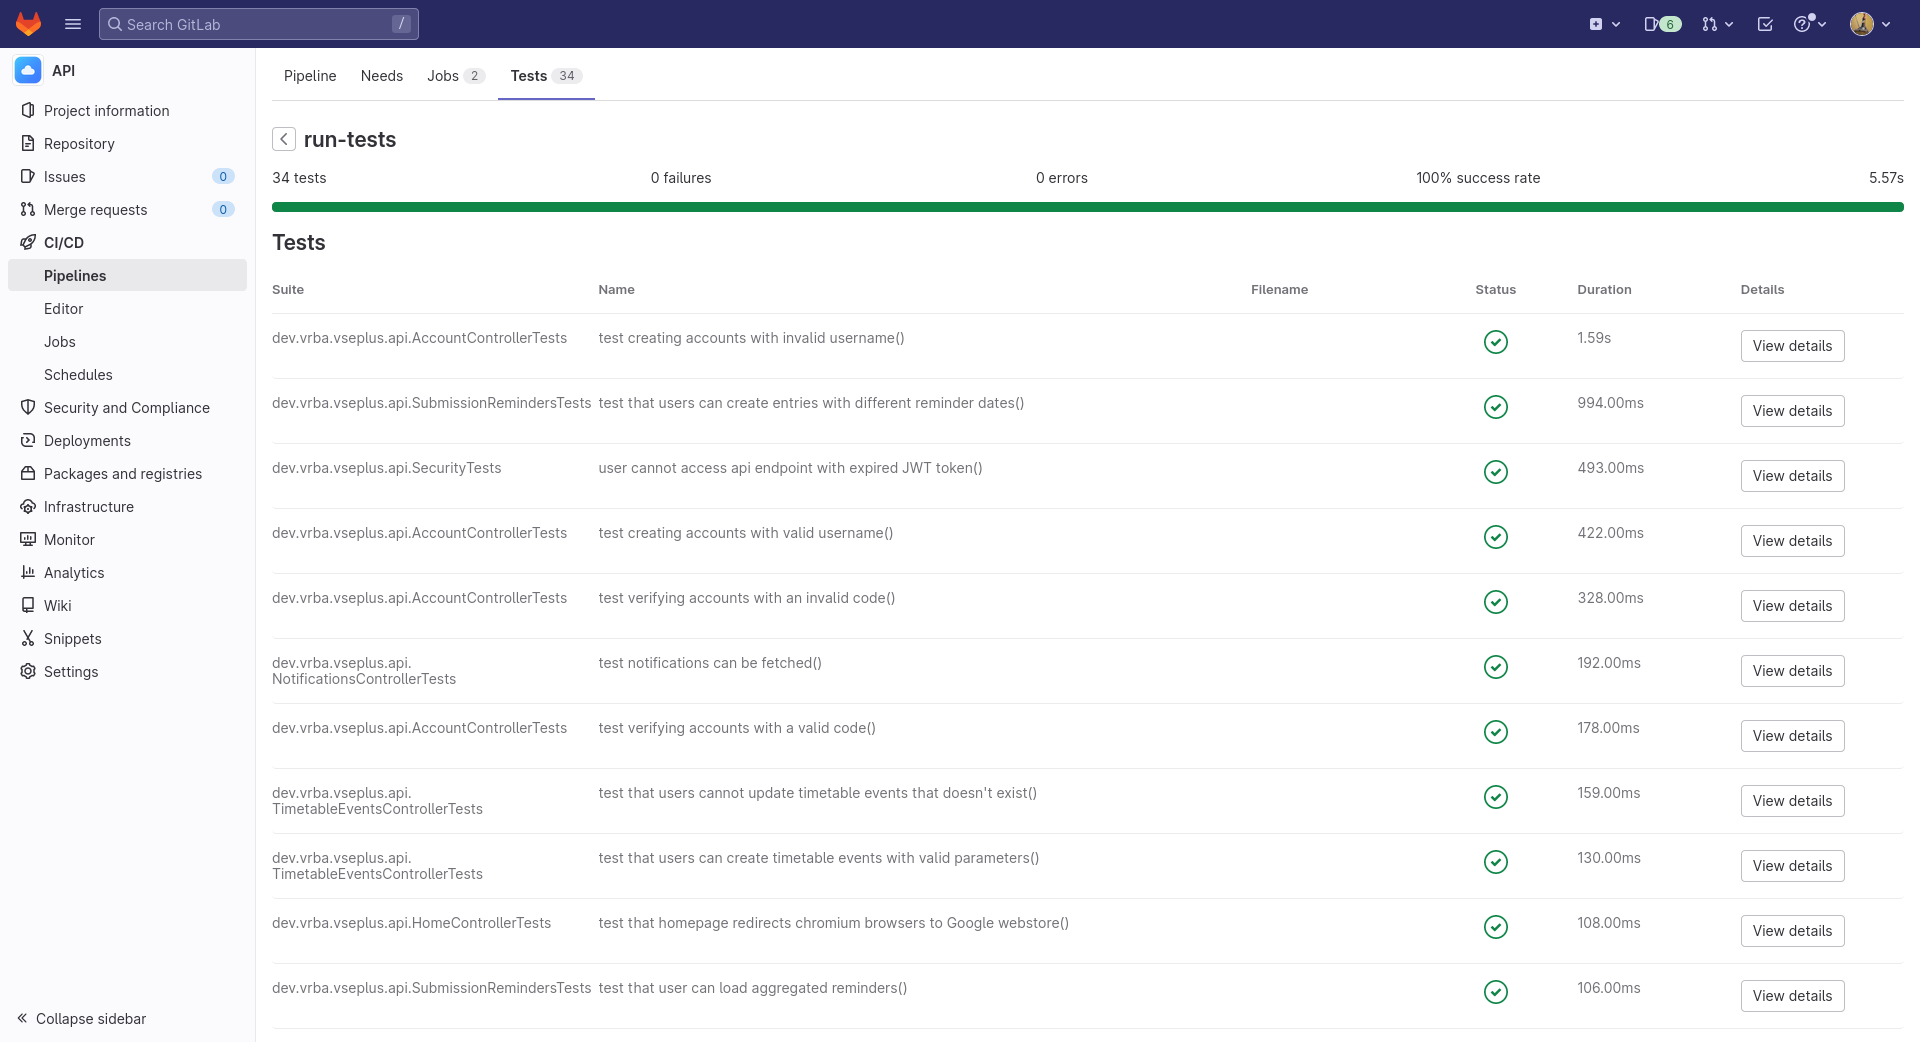
\includegraphics[width=\textwidth]{img/gitlab-ci-junit.png}
    \caption{Výsledky spuštění JUnit testů v~platformě GitLab (vlastní zpracování)}
    \label{fig:gitlab-ci-junit}
\end{figure}
 
\section{Nasazení aplikace}

Pro nasazení podpůrného serveru je potřeba zvážit hned několik faktorů, které hrají roli. 
Prvním z~těchto faktorů je otázka jak bude probíhat distribuce softwaru, tj. jak se bude sestavovat aplikační balíček a jak se bude tento aplikační balíček spouštět. 
Dalším faktorem pro zvážení před nasazením aplikace je provozní cena. Jelikož se jedná o~dlouhodobě běžící projekt s~nulovou návratností a protože rozšíření je poskytováno zcela zdarma, byla vyvinuta snaha snížit náklady spojené s~provozem aplikace na minimum.

\subsection{Výběr hostingu}

Pro distribuci aplikace byl z~důvodu přenositelnosti řešení zvolen nástroj Docker pro kontejnerizaci řešení. To značně zjednodušilo výběr platformy pro hosting, protože se od sebe poskytovaná řešení liší z~pohledu běhového prostředí pouze minimálně v~porovnání s~řešeními pro hosting nativních Java aplikací.

Hlavním rozdílem mezi platformami byl způsob stanovení ceny. U~flexibilních cloudových poskytovatelů jako je Amazon Web Service a řešení ESC (Elastic Container Service) nebo Google Cloud Run je cena počítána dynamicky podle míry využití poskytovaných zdrojů, které jsou alokovány dynamicky. U~ostatních platforem je model výpočtu výsledné ceny více přímočarý, protože se jedná o~fixní celkovou částku za předem definovanou statickou výpočetní kapacitu.

Po odhadu potřebných výpočetních zdrojů, které byly stanoveny pomocí průměru 5 měření metrik nástroje Micrometer byla odhadnuta cena provozu u~jednotlivých platforem. Po vyhodnocení vyšla jako nejlepší varianta, která splňovala všechny kladené požadavky za nejmenší cenu platforma Digital Ocean Droplets, která umožňuje hosting docker kontejneru s~aplikací s~jedním vCPU a 512 MB RAM za 4 USD měsíčně. Digital Ocean zároveň poskytuje slevu pro studenty v~podobě kreditů, které po uplatnění sníží výsledné měsíční cenu za provoz pod 1 USD.  


\subsection{Využítí technologie Docker}\label{sec:docker}

Docker je technologie pro virtualizaci a izolaci běhového prostředí aplikací za pomocí takzvaných kontejnerů. Tyto kontejnery jsou alternativou k~tradičním enterprise nástrojům pro virtualizaci jako například VMware nebo KVM. Kontejnery se od virtuálních počítačů liší tím, že s~hostujícím operačním systémem sdílí systémové jádro a jsou tedy mnohem méně náročné na systémové prostředky pro chod virtualizovaného systému, protože nedochází k~simulaci hardwarových prostředků a operačního systému s~překladem systémových volání \cite[kap. 1]{kane_docker_2018}.

Docker umožňuje snadno vytvářet, spravovat a sdílet tyto kontejnery, což výrazně usnadňuje proces distribuce softwarových balíčků a jejich závislostí, protože je možné celou aplikace včetně všech závislostí zabalit do připraveného kontejneru s~nakonfigurovaným běhovým prostředím. 

Docker pracuje s~konceptem takzvaných images, které si lze představit jako šablonu pro vytváření kontejnerů. Tyto image jsou projekcí stavu souborového systému a z~jedné image je možné vytvořit neomezené množství kontejnerů, které pak následně nástroj Docker spravuje. 

\subsection{Automatické sestavování Docker image pomocí GitLab CI/CD}

Pro sestavení Docker image obsahující zdrojové kódy a běhové prostředí pro podpůrný webový server je možné využít kombinaci nástrojů GitLab CI/CD a GitLab Container Registry. GitLab Container Registry je platforma implementující protokol pro vytváření a publikaci repozitářů pro Docker image.

\subsection{Zdrojové kódy a historie změn}

Aktuální verze zdrojových kódu a historie změn pro podpůrný webový server je dostupná jako repozitář na platformě GitLab, který je k~dispozici ve webovém rozhraní platformy GitLab na URL adrese \url{https://gitlab.com/vse-plus/api}.
\chapter{Implementace rozšíření do webových prohlížečů}

Zatímco podpůrný webový server zajišťuje potřebnou infrastrukturu pro ukládání uživatelských dat, správu uživatelských účtů a rozesílání emailů, klíčovou částí projektu je rozšíření do webových prohlížečů, které zajišťuje integraci přidaných funkcionalit do webového rozhraní školního informačního systému InSIS.

Webové rozšíření jsou softwarové balíčky, které umožňují přidávat nové funkce do webových prohlížečů jako například Google Chrome, Mozilla Firefox nebo Opera. Dále je možné pomocí rozšíření do prohlížečů měnit chování stránek pomocí injekce vlastních skriptů a kaskádových stylů.

Právě prostřednictvím injekce vlastních skriptů a kaskádových stylů jsou implementované funkcionality poskytované rozšířením VŠE+.

\section{Manifest rozšíření}

Základní částí každého rozšíření do webových prohlížečů, bez které nemůže rozšíření vzniknout, je soubor \code{manifest.json}. Jedná se o~konfigurační soubor, který definuje všechny potřebné atributy od názvu rozšíření, popisu, autora až po definice oprávnění a specifikaci přidaných funkcí a skriptů. 

Jednou z překážek při vývoji rozšíření, která jsou podporována více než jedním webovým prohlížečem je zajištění kompatibility mezi běhovým prostředím a verzí manifestu. Jelikož webový prohlížeč Mozilla Firefox v době psaní této práce nepodporuje manifest s verzí 3 a zároveň webové prohlížeče založené na technologii Chrome nepodporuje manifest s verzí 2, bylo potřeba tyto manifest soubory oddělit do 2 verzí. V projektu se jedná o soubory `public/manifest-chrome.json` pro webové prohlížeče založené na technologii Chrome a soubor `public/manifest-firefox.json` pro webový prohlížeč Firefox.

\section{Content script}

Jedním ze základních stavebních kamenů rozšíření je content script, což je JavaScriptový kód, který se injektuje do stránek informačního systému InSIS, který na základě detekovaného modulu a uživatelských preferencí spouští jednotlivé části rozšíření, které poskytují rozšíření pro vybrané moduly informačnícho systému InSIS. Je tedy možné na tento content script pohlížet jako na vstupní bod celého rozšíření.

Níže jsou uvedeny a vysvětleny některé z~relevantních částí kódu, které se v~rámci tohoto vstupního bodu volají.

\begin{lstlisting}[
label={code:content-script-data-loading}, 
caption={Načítání dat z~paměti prohlížeče v~rámci content scriptu (vlastní zpracování)}
]
const items = await browser.storage.local.get([
    "authentication",
    "preferences",
    "notificationsTimestamp"
]);

const authentication: Authentication = items["authentication"] ?? {
    authenticated: false,
    username: null,
    token: null
};

const preferences: Preferences = items["preferences"] ?? {
    features: {}
};

  const notificationsTimestamp = new Date(items["notificationsTimestamp"] || 0);
\end{lstlisting}

 Část kódu ve výpise \ref{code:content-script-data-loading} načítá z~paměti prohlížeče uložené informace o~přihlášení uživatelské, uživatelské preference a časovou značku posledního zobrazeného oznámení. Tyto informace jsou uloženy v~interním úložišti prohlížeče a přístup k~těmto datům rozšíření je omezený pouze na součásti rozšíření definované v~manifestu.
V~dalších částech kódu se pak načtené informace využívají pro rozhodnutí, jestli se mají přidané funkcionality spustit.

\begin{lstlisting}[
label={code:preferences-content-script}, 
caption={Vyhodnocení, jestli je vybraná funkcionalita zapnutá v~rámci uživatelských preferencí (vlastní zpracování)}
]
if (
    isFeatureEnabled(preferences, "enhanced-timetable") && 
    window.location.href.includes("/rozvrhy_view.pl")
) {
    await enableEnhancedTimetable(authentication);
}
\end{lstlisting}

Výpis \ref{code:preferences-content-script} zachycuje část kódu, ve které se nejdříve vyhodnotí, jestli má uživatel zapnutou funkcionalitu pro vylepšení rozvrhu a poté proběhne kontrola adresy URL, jestli obsahuje textový řetězec \code{"/rozvrhy\_view.pl"}, jehož výskyt implikuje, že se uživatel nachází na stránce s~rozvrhem hodin.

Samotná funkce \code{isFeatureEnabled} pak pouze kontroluje předaný parametr, kde zjistí, jestli je jeho hodnota v~rámci uživatelských preferencí nastavena na pravdivou hodnotu.

\begin{lstlisting}[label={code:is-feature-enabled}, caption={Definice funkce \code{isFeatureEnabled} (vlastní zpracování)}]
export const isFeatureEnabled = 
    (preferences: Preferences, feature: string): boolean => {
        // Fallback to all features enabled by default for discoverability
        if (!preferences ||  !Object.keys(preferences.features).includes(feature)) {
            return true;
        }
    
        return preferences.features[feature];
    }
\end{lstlisting}

Jak napovídá komentář na 3. řádku, pokud není uživatelská preference pro danou funkcionalitu definovaná, aplikace se chová stejně, jako kdyby danou funkcionalitu uživatel zapnul.

\subsection{Detekce podstránek}

Jednou z~úloh content scriptu je detekce v~jakém modulu informačního systému InSIS se uživatel právě nachází pomocí URL adresy. Tuto adresu je možné získat z~atributu \code{href}, který je definovaný v~rámci globálního objektu \code{window.location}. Tento objekt se v~programovacím jazyce JavaScript a posléze TypeScript využívá pro získání aktuální adresy URL, na které se uživatel webového prohlížeče nachází.

\todo{Ocitovat MDN a window.location nebo Chernyho}

Detekci modulu, ve kterém se uživatel informačního InSIS nachází je možné definovat pomocí tabulky \ref{tab:url-patterny}, která obsahuje mapování textových řetězců, které jsou unikátní pro každý zmíněný modul.

\begin{table}[htbp!]
\centering
\caption{Textové řetězce implikující modul systému InSIS}\label{tab:url-patterny}
    \begin{tabular}{ll}
        \toprule
        \textbf{Textový řetězec v~URL} & \textbf{Modul systému InSIS} \\
        \midrule
        \verb|/rozvrhy_view.pl| & Zobrazení rozvrhu \\
        \verb|/vyber_cviceni.pl| & Registrace rozvrhových akcí \\
        \verb|/odevzdavarny.pl| & Odevzdávárny \\
        \bottomrule
    \end{tabular}
\end{table}

\subsection{Moduly content scriptu}

Zdrojový kód souboru \code{content\_script.tsx}, který je zaregistrovaný jako vstupní bod rozšíření, sám o~sobě neobsahuje implementaci přidaných funkcionalit, které byly vymezeny v~kapitole \ref{chap:navrh-a-specifikace}. Namísto toho po detekci modulu systému InSIS spouští jednotlivé moduly rozšíření, které implementují potřebnou logiku a uživatelské rozhraní pro přidané funkcionality. Tyto moduly se nachází ve složce \code{src/modules} a každý tento modul je představován složkou, která obsahuje soubor \code{index.ts}, alternativně \code{index.tsx}, který exportuje funkci pro zavedení funkcionality do stránky informačního systému. 

Například pro zavedení funkcionality zobrazení náhledu rozvrhu při registraci rozvrhových akcí se z~content scriptu volá funkce \code{enableTimetablePreview}, která je definovaná v~souboru \code{src/modules/timetable-preview/index.tsx}.

\subsection{Implementace náhledu rozvrhu při registraci rozvrhových akcí}

Náhled rozvrhu při registrací je modul rozšíření, který se volá z~content scriptu po detekci příslušného textového řetězce v~URL adrese. Vstupním bodem tohoto modulu je funkce \code{enableTimetablePreview}, která očekává 1 argument typu boolean, který určuje, zdali se mají graficky odlišit hodiny s~detekovanou kolizí napříč již zaregistrovanými rozvrhovými akcemi.

\begin{lstlisting}[label={code:enable-timetable-preview}, caption={Definice funkce \code{enableTimetablePreview} (vlastní zpracování)}]
const createContainer = (): HTMLDivElement => {
    const container = document.createElement("div");
    document.body.appendChild(container);
    return container;
};

export const enableTimetablePreview = async (hideCollisions: boolean) => {
    const container = createContainer();
    const root = createRoot(container)

    root.render(
        <React.StrictMode>
            <TimetablePreview hideCollisions={hideCollisions}/>
        </React.StrictMode>
    );
}
\end{lstlisting}

V~této funkci se nejprve vytvoří container, ve kterém se zavede kořenový element pro renderování React komponent, v~rámci kterého se vyrenderuje komponenta \code{TimetablePreview}, která zabaluje logiku a uživatelské rozhraní spojené s~načtením, zpracováním a následným zobrazením rozvrhových akcí. 

\subsubsection{Načítání již zaregistrovaných rozvrhových akcí}

Jelikož školní informační systém InSIS nemá na rozdíl od informačních systémů některých jiných škol\footnote{Příkladem může být informační systém KOS, který využívá ČVUT} dostupné API, ze kterého by bylo možné načítat již zaregistrované rozvrhové akce ve strojově čitelném formátu. Je tudíž potřeba tuto informaci získat pomocí extrakce informací přímo z~HTML kódu stránek systému InSIS. 

Prvním krokem pro extrakci registrovaných hodin je asynchronní načtení stránky s~registracemi na pozadí pomocí technologie AJAX. To je realizované v~rámci pomocné funkce \code{loadCurrentTimetable}. Implementace zmíněné pomocné funkce je možné vidět ve výpise \ref{code:load-current-timetable}.

\begin{lstlisting}[label={code:load-current-timetable}, caption = {Implementace funkce \code{loadCurrentTimetable} (vlastní zpracování)}]
export const loadCurrentTimetable = async () => {
    const url = "https://insis.vse.cz/auth/student/registrace.pl?lang=cz";
    const source = await fetch(url)
        .then(response => response.text())
        .then(response => parseTimetable(response));

    return source;
};
\end{lstlisting}

Volaná funkce \code{fetch} je součástí API internetových prohlížečů a umožňuje odesílání AJAX požadavků na pozadí. Návratovou hodnotou této funkce je instance datového typu \code{Promise}. Tento datový typ je monadickým zapouzdřením pro hodnoty, které v~době volání obslužného kódu nejsou ještě k~dispozici, a jejichž hodnota je získána asynchronně. V~případě funkce \code{fetch} je hodnota v~podobě HTTP odpovědi dostupná až v~momentě, kdy je odeslaný HTTP požadavek obsloužen serverem.

Datový typ \code{Promise} umožňuje definovat sérii operací, které se mají na výsledné hodnotě vykonat v~momentě kdy je dostupná. Tyto operace se na datovém typu \code{Promise} definují pomocí metody \code{Promise.then}, která jako první argument přijímá mapující funkci, která převádí jeden generický datový typ na jiný. Tuto funkci předanou jako parametr je možné definovat jako datový typ \code{(A) => B}. Výsledným datovým typem volání funkce \code{Promise<A>.then((A) => B)} je pak \code{Promise<B>} \cite[kap. 13.2]{flanagan_javascript_2020}.

Tato vlastnost, kdy volání vrací stejný generický datový typ umožňuje vytváření komplexních kompozic asynchronních volání za pomocí jednoduchého, deklarativního kódu, který se snadno čte a udržuje. Další výhodou využití datového typu \code{Promise} je jeho podpora na úrovni jazyka v~podobě klíčových slov \code{async} a \code{await}, které umožní ještě dále zjednodušit asynchronní kód. 

V~ukázce zdrojového kódu zachycující funkci \code{loadCurrentTimetable} je možné vidět kompozici 3 asynchronních funkcí. První funkcí je již zmíněná funkce \code{fetch}, která slouží pro vykonání HTTP požadavku pomocí technologie AJAX. Další funkcí je funkce \code{Response.text()}, která předevede odpověď na HTTP požadavek v~podobě instance třídy \code{Response} na textový řetězec. Poslední funkcí v~kompozici je pak funkce \code{parseTimetable}, která zajišťuje zpracování HTML kódu v~odpovědi a extrakci rozvrhových akcí.

Ve funkci \code{parseTimetable} nejdříve proběhne převedení zdrojového HTML do stromové reprezentace DOM. V~rámci DOM reprezentace je pak nalezena tabulka s~rozvrhovými akcemi a proběhne zpracování všech řádků této tabulky. U~každého řádku dojde k~extrakci následujících informací: typ rozvrhové akce, cvičení nebo blokovou akci, den v~týdnu, čas začátku a čas konce. 

Po načtení a extrakci již zapsaných rozvrhových akcí proběhne extrakce rozvrhových akcí, mezi kterými si uživatel volí. Extrakce informací z~webové stránky probíhá obdobně jako u~již zaregistrovaných rozvrhových akcí. Nejprve je nalezena tabulka s~rozvrhovými akcemi a následně je postupně zpracován každý řádek této tabulky. Z~každého řádku je pomocí regulárních výrazů vyextrahována informace o~dni v~týdnu ve kterém daná rozvrhová akce probíhá a čas začátku a konce. V~rámci zpracování DOM reprezentace HTML stránky je každý řádek anotován speciálním atributem \url{data-timetable-highlight}, jehož hodnota je pro každý řádek nastavena na jeho unikátní pořadové číslo, aby bylo možné později efektivně napojit události najetí myší na řádek tabulky s~vyznačením konkrétní hodiny v~zobrazeném náhledu.

Po sestavení potřebného datového modelu dojde k~vyrenderování kořenové React komponenty \code{TimetablePreview}, která zapouzdřuje zobrazení náhledu zaregistrovaných a dostupných rozvrhových akcí.

\subsection{Implementace připomenutí odevzdáváren a export do externího kalendáře}
    
Základní částí implementace připomenutí odevzdáváren je zpracování tabulky s~odevzdávárnami v~rozhraní informačního systému InSIS, které probíhá po detekci stránky a spuštění modulu content scriptu. Tabulka s~aktivními odevzdávárnami je zpracována řádek po řádku, kdy u~každé odevzdávárny probíhá extrakce informací přes iteraci DOM stromové struktury a regulární výrazy. Extrahují se informace o~názvu předmětu, názvu odevzdávárny, datumu uzavření a unikátním ID odevzdávárny.

Po dokončení zpracování a extrakce dat z~tabulky s~aktivními odevzdávárnami proběhne rozšíření HTML tabulky s~odevzdávárnami o~2 nové sloupce. První přidaný sloupec obsahuje ikonu pro indikaci jestli je pro danou odevzdávárnu již vytvořené upozornění, a druhý sloupec obsahuje sadu ikon pro export do externího kalendáře. Oba stavy ikony pro připomenutí odevzdáváren zobrazují obrázky \ref{fig:pripomenuti-off} a \ref{fig:pripomenuti-on}.

Po kliknutí na jednu z~ikon pro správu připomenutí se vytvoří container element s~unikátním identifikátorem \code{submission-reminders-overlay}, v~rámci kterého se zaregistruje kořenový element pro vykreslení React aplikace. Tato React aplikace obsahuje komponenty pro výběr časů připomenutí a správu již zaregistrovaných připomenutí. 

\begin{figure}[H]\centering
    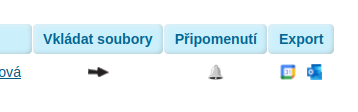
\includegraphics[width=0.33\textwidth]{img/pripomenuti-off.png}
    \caption{Ikona pro připomenutí odevzdáváren v~neaktivním stavu (vlastní zpracování)}
    \label{fig:pripomenuti-off}
\end{figure}

\begin{figure}[H]\centering
    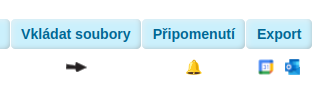
\includegraphics[width=0.33\textwidth]{img/pripomenuti-on.png}
    \caption{Ikona pro připomenutí odevzdáváren v~aktivním stavu (vlastní zpracování)}
    \label{fig:pripomenuti-on}
\end{figure}

Výběr času připomenutí je realizován pomocí dialogového okna, které obsahuje seznam zaregistrovaných časů připomenutí a sadu tlačítek pro registraci dalších časů připomenutí. Uživatelské rozhraní tohoto dialogového okna je možné vidět na obrázku \ref{fig:pripomenuti-modal}, který zobrazuje nastavení pro odevzdávárnu se dvěma již zaregistrovanými časy připomenutí.

\begin{figure}[H]\centering
    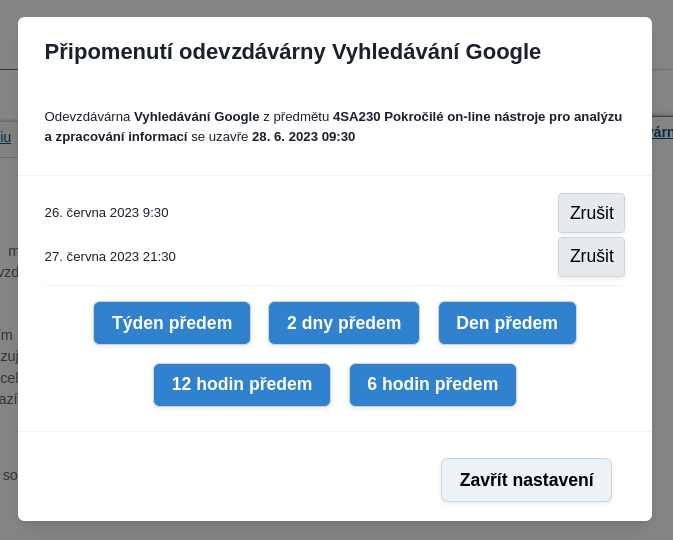
\includegraphics[width=0.66\textwidth]{img/pripomenuti-modal.png}
    \caption{Dialogové okno pro nastavení časů připomenutí (vlastní zpracování)}
    \label{fig:pripomenuti-modal}
\end{figure}

\subsection{Implementace vylepšeného rozvrhu}

Asi nejvíce komplexní částí celého rozšíření je modul pro vylepšený rozvrh, jehož funkce jsou podrobněji popsané v~kapitole \ref{sec:vylepseny-rozvrh}. Tato komplexita vychází především z~množství zpracovávaných informací a z~rozmanitosti uživatelského rozhraní, které se musí flexibilně přizpůsobovat různým situacím. 

Ihned po detekci že se uživatel nachází v~modulu osobní rozvrh dochází k~načtení a zpracování tabulky s~rozvrhem hodin a tabulky s~poznámkami k~hodinám, ze kterých proběhne extrakce informací, podobně jako tomu bylo u~ostatních popisovaných modulů. Jako první proběhne zpracování hodin v~zobrazeném rozvrhu. 

Původní rozvrh poskytovaný informačním systémem InSIS je navržený jako HTML tabulka, která obsahuje sloupce pro každých 5 minut v~časovém okně od 7:30 do 19:30. Každá hodina zanesená v~tomto rozvrhu je reprezentovaná pomocí buňky tabulky, která přesahuje přes počet sloupců odpovídající délce trvání v~minutách děleno pěti. Každá taková buňka je barevně odlišena podle typu rozvrhové akce (zdali se jedná o~přednášku, cvičení nebo blokovou akci). Tato barva je definována pomocí CSS tříd, které jsou aplikovány na buňku a které je možné využít pro extrakci typu každé buňky, respektive každé rozvrhové akce. U~každé z~rozvrhových akcí dochází k~extrakci místnosti, předmětu, vyučujícího, dne v~týdnu, délky trvání, typu rozvrhové akce a času začátku dané akce.

Poté co proběhne zpracování a extrakce informací z~původního rozvrhu dochází k~zpracování poznámek k~rozvrhu, které se nachází ve spodní části obrazovky pod rozvrhem. Klíčovým typem poznámek k~hodinám je definice volných dní, které jsou detekovány pomocí regulárního výrazu. Dalším důležitých typem poznámky jsou datumy konání v~případě, že se jedná o~blokovou akci. Tento typ poznámek se týká především mimosemestrálních kurzů a seminářů, které probíhají pouze v~některých týdnech.

Zpracované informace z~původního rozvrhu a z~poznámek k~rozvrhu jsou následně zkombinovány do pole objektů, obsahující datovou reprezentaci rozvrhových akcí a k~nim přidružené zpracované poznámky. Po spojení dat dochází k~odstranění původního rozvrhu a vytvoření kořenového prvku pro vyrenderování React komponenty s~upraveným rozvrh. Této komponentě jsou jako vstupní parametry předány zkombinovaná data společně s~tokenem pro autentikaci na podpůrném serveru pro načítání uživatelských poznámek v~rozvrhu. Kořenový element obsahuje pouze tuto jedinou komponentu \code{<Timetable/>}, která se následně stará o~celý proces načítání a renderování dat v~rozvrhu.

V~komponentě \code{<Timetable/>} dochází k~načtení poznámek z~podpůrného serveru pomocí technologie AJAX a~vytvoření kontextu pro každý týden výukového období. Tato komponenta je tvořena několika dílčími komponentami. První z~těchto komponent je uživatelské rozhraní pro zobrazení a~přepínání aktuálně zobrazeného týdne. Ve výchozím stavu se zobrazuje aktuální týden, pokud je aktuální den v~týdnu v~rozpětí pondělí - pátek. Pokud je aktuální den sobota nebo neděle, zobrazuje se ve výchozím stavu týden následující po aktuálním týdnu.   

\begin{figure}[H]\centering
    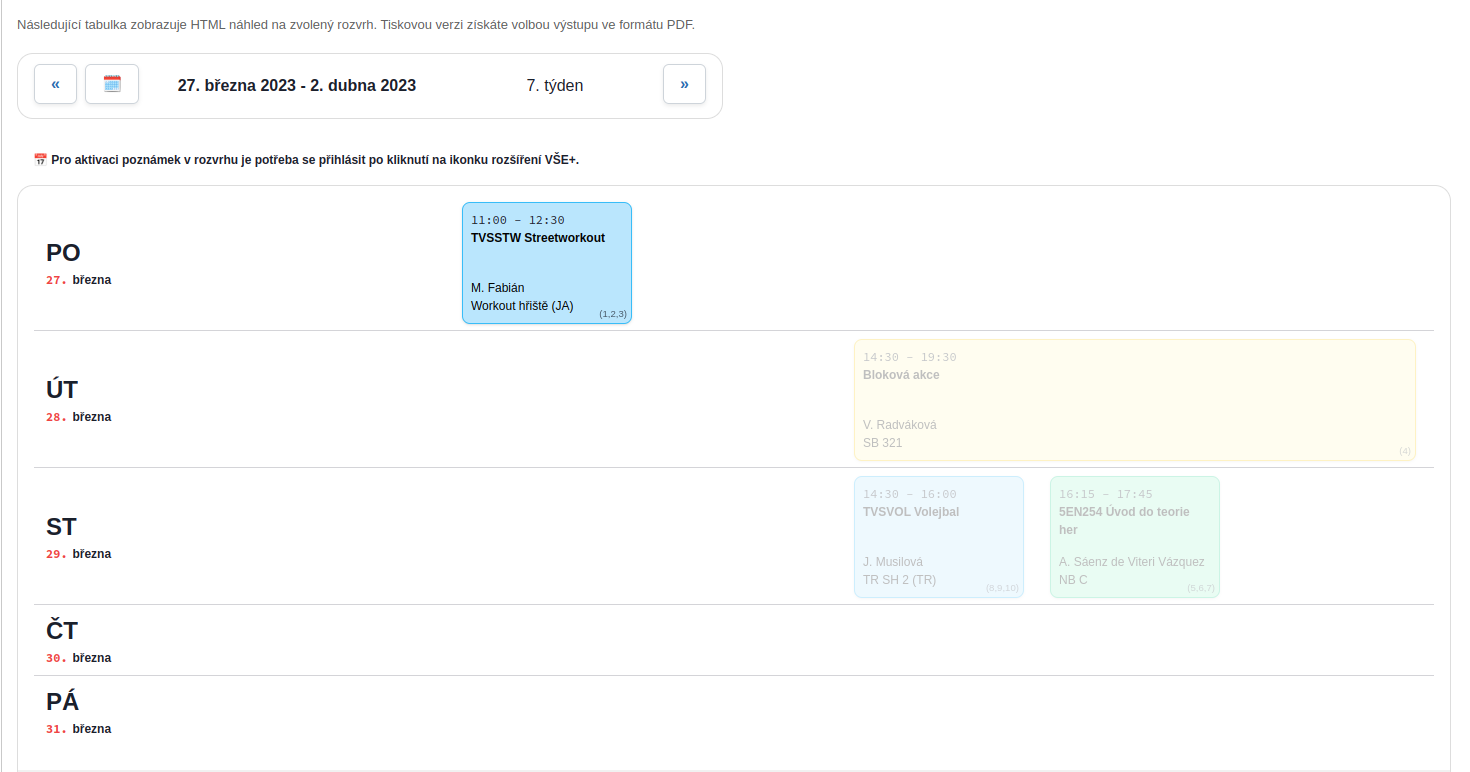
\includegraphics[width=\textwidth]{img/rozvrh-volne-dny.png}
    \caption{Grafické odlišení volných dní v~rozvrhu (vlastní zpracování)}
    \label{fig:rovrh-volne-dny}
\end{figure}

\subsection{Implementace přihlášení do rozšíření}

Přihlášení do webového rozšíření je společně s~nastavením uživatelských preferencí jedinou částí rozšíření, která není implementovaná v~podobě modulu content scriptu. Namísto toho je tato část rozšíření implementovaná jako popup obrazovka, která se zobrazí po kliknutí na ikonu rozšíření jak zobrazují obrázky \ref{fig:prihlaseni-1} a \ref{fig:prihlaseni-2}.

\begin{figure}[H]\centering
    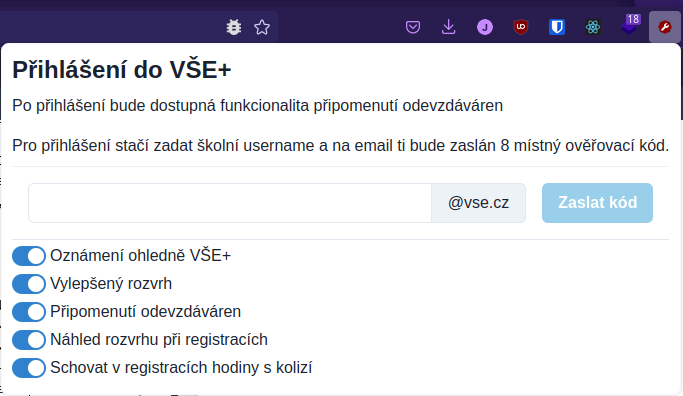
\includegraphics[width=\textwidth]{img/prihlaseni-vse-plus.png}
    \caption{Popup obrazovka pro zadání emailové adresy (vlastní zpracování)}
    \label{fig:prihlaseni-1}
\end{figure}


\begin{figure}[H]\centering
    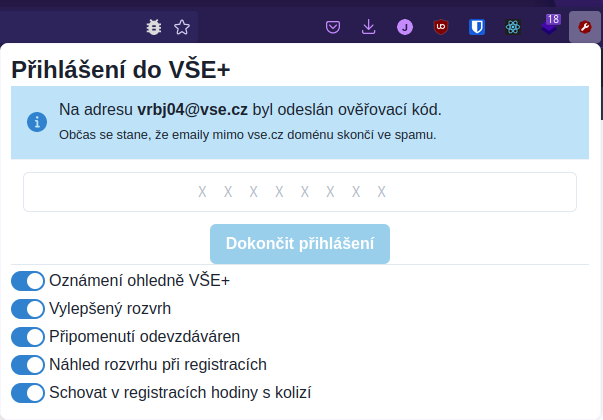
\includegraphics[width=\textwidth]{img/prihlaseni-vse-plus-kod.png}
    \caption{Popup obrazovka pro zadání ověřovacího kódu (vlastní zpracování)}
    \label{fig:prihlaseni-2}
\end{figure}

Tato popup obrazovka je zaregistrovaná v~manifestu rozšíření. Ve verzi 2 manifestu se jedná o~klíč \code{browser\_action}, ve verzi 3 manifestu se jedná o~klíč \code{action}. V~rámci tohoto klíče se definují 2 vlastnosti. První vlastností je \code{default\_popup}, který představuje cestu ke~vstupnímu HTML souboru který se má v~rámci popup obrazovky rozšíření zobrazit. Tato cesta je relativní vůči kořenovému adresáři složky se sestaveným rozšířením a v~případě rozšíření VŠE+ se jedná o~soubor s~názvem \code{popup.html}. Druhou z~vlastností je \code{default\_title}, která představuje nadpis, který se má zobrazit po najetí myší na ikonu rozšíření v~liště prohlížeče.

\todo{Ocitovat extension manifest na web dev}

Soubor \code{popup.html}, na který se v~rámci manifestu odkazuje sekce pro definici popup stránky je velice jednoduchý a~kromě základních definic HTML dokumetu obsahuje pouze 2 důležité části. Jednou částí je definice \code{<div>} elementu, který slouží jako kořenový element pro vložení React aplikace. Další částí jsou importy sestavených JavaScript souborů, které zajistí vykreslení React aplikace v~rámci definovaného kořenového elementu. Prvním importem je soubor \code{js/vendor.js}, který obsahuje kód závislostí a knihoven, zejména kód pro knihovnu React.js a sadu komponent Chakra UI. Druhým souborem je \code{js/popup.js}, který obsahuje zkompilovaný TypeScript kód pro vyrenderování grafického rozhraní pro přihlášení a uživatelské preference společně s~implementací přidružené logiky pro načítání a ukládání uživatelských preferencí, odesílání autentikačních požadavků na podpůrný webový server a ukládání vygenerovaného autentikačního tokenu.

\subsection{Uživatelské preference a aktivace funkcionalit}

Jak je možné vidět na obrázcích \ref{fig:prihlaseni-1} a \ref{fig:prihlaseni-2}, uživatel má možnost si v~rámci popup stránky rozšíření zvolit, které z~přidaných funkcionalit jsou zapnuté a které nikoliv. Tyto preference jsou definované v~rámci React komponenty \url{src/components/Preferences.tsx}, kde jsou součástí objektu s~názvem pro zobrazení pro uživatele.

Celkem je definovaných 5 přepínačů, které je možné vypnout nebo zapnout podle preference uživatele rozšíření. Definice klíčů a přidružených popisů funkcionalit je možné vidět ve výpise \ref{code:preferences-features}

\begin{lstlisting}[
    label={code:preferences-features},
    caption={Definice přepínačů a přidružených popisů funkcionalit (vlastní zpracování)}
]
const names: Record<string, string> = {
    "notifications": "Oznámení ohledně VŠE+",
    "enhanced-timetable": "Vylepšený rozvrh",
    "submission-reminders": "Připomenutí odevzdáváren",
    "timetable-preview": "Náhled rozvrhu při registracích",
    "timetable-preview:hide-collisions":
        "Schovat v~registracích hodiny s~kolizí"
}
\end{lstlisting}

Jak je vidět u~posledního definovaného přepínače, pokud se jedná o~přepínač závislý na jiném přepínači, v~tomto případě konkrétně o~přepínač \url{timetable-preview:hide-collisions}, který je závislý na přepínači \url{timetable-preview}, je klíč přepínače oddělen dvojtečkou, což umožňuje validaci, že funkcionalita, na které je přepínač závislý je zapnutá. V~případě, že daná funkcionalita je uživatelem vypnutá, je zablokována možnost měnit závislé přepínače. Tuto situaci zachycuje obrázek \ref{fig:zavisle-prepinace}, kde je možné vidět zablokování změny přepínače "Schovat v~registracích hodiny s~kolizí", protože přepínač "Náhled rozvrhu při registracích", na kterém je druhý přepínač závislý, se nachází ve vypnutém stavu.

Detekce jestli se jedná o~závislý přepínač a jestli má být zablokována možnost měnit hodnotu se vyhodnocuje pro každý přepínač pomocí kódu ve výpise \ref{code:user-preferences-disabled}.

\begin{lstlisting}[label={code:user-preferences-disabled}, caption={Detekce stavu závislého přepínače (vlastní zpracování)}]
const disabled = feature.includes(":") && !isFeatureEnabled(
    preferences,
    feature.split(":")[0]
)
\end{lstlisting}

Proměnná \code{feature} obsahuje textový řetězec s~klíčem přepínače a proměnná \code{preferences} obsahuje načtené preference uživatele. V~prvním kroce proběhne kontrola, že klíč obsahuje znak dvojtečky a pokud ano, klíč se rozdělí na pole textových řetězců podle dvojtečky. Tedy například u~klíče \code{"timetable-preview:hide-collisions"} by došlo k~rozdělení na pole \code{["timetable-preview", "hide-collisions"]}. Z~tohoto pole se pak vezme první prvek, v~tomto případě \code{"timetable-preview"} a proběhne kontrola, jestli je přepínač s~tímto klíčem přepnutý do vypnutého stavu.


Ukládání a načítání uložených uživatelských preferencí je implementováno prostřednictvím \code|browser.storage|, které bylo zmíněno v~předchozích kapitolách. Při prvním renderu uživatelských preferencí dojde k~načtení uložených hodnot pomocí volání funkce \url{browser.storage.local.get("preferences")}. Pokud nejsou uložené preference nalezeny, je vrácen prázdný objekt, který v~důsledku chování implementace funkce \code{isFeatureEnabled} popsané ve výpise \ref{code:is-feature-enabled} způsobí, že všechny přepínače se nachází v~zapnutém stavu. 

\begin{lstlisting}[label={code:is-feature-enabled}, caption={Definice funkce \code{isFeatureEnabled} (vlastní zpracování).}]
export const isFeatureEnabled = (preferences: Preferences, feature: string): boolean => {
    // Fallback to all features enabled by default for discoverability
    if (!preferences || !Object.keys(preferences.features).includes(feature)) {
        return true;
    }

    return preferences.features[feature];
};
\end{lstlisting}

\section{Sestavování a distribuce rozšíření}

Standardním postupem distribuci rozšíření do webových prohlížečů je využití internetových obchodů, které tyto rozšíření nabízí. Tyto obchody jsou většinou spojené přímo s~konkrétním internetovým prohlížečem a jsou provozovány výrobcem internetového prohlížeče. 

Pro distribuci byly zvoleny 2 hlavní internetové obchody s~rozšířeními do webových prohlížečů: Google Web Store a Firefox Addons. Google Web Store je internetový obchod provozovaný společností Google ve kterém jsou k~dispozici rozšíření a témata do webového prohlížeče Google Chrome a ostatních prohlížečů založených na technologii Chromium. 
Výhodou podpory ostatních prohlížečů je, že uživatelé alternativních prohlížečů jako je zejména prohlížeč Opera nebo Microsoft Edge si mohou rozšíření nainstalovat z~obchodu Google Web Store bez nutnosti instalace webového prohlížeče Google Chrome. Druhým zmíněným obchodem, který byl zvolen pro distribuci webového rozšíření VŠE+ je internetový obchod Firefox Addons, který je provozovaný společností Mozilla, která zároveň vyvíjí webový prohlížeč Mozilla Firefox, pro který je tento internetový obchod určen. 

Mezi oběma zmíněnými internetovými obchody existuje celá řada podobností a~rozdílů. Jedním z~prvních rozdílů, se kterými přijde vývojář do styku, je nutnost koupě vývojářské licence pro obchod Google Web Store. Tato licence stojí v~době psaní této práce 5 amerických dolarů a~bez této licence není možné publikovat do obchodu Google Web Store žádný obsah. Naproti tomu publikování webových rozšíření a témat do obchodu Firefox Addons nevyžaduje licenci a~může být realizováno bezplatně.       

Jednou z~výhod využití zmíněných internetových obchodů jsou metriky, které tyto obchody poskutují. Autorům rozšíření dodávají podrobné statistiky o~počtu instalací, demografii uživatelů rozšíření a rozložení nainstalovaných verzí rozšíření. Tyto statistiky je možné vidět v~panelu vývojáře a zmíněné obchody umožňují stažení zdrojových dat v~podobě csv souboru.

\begin{figure}[htbp!]\centering
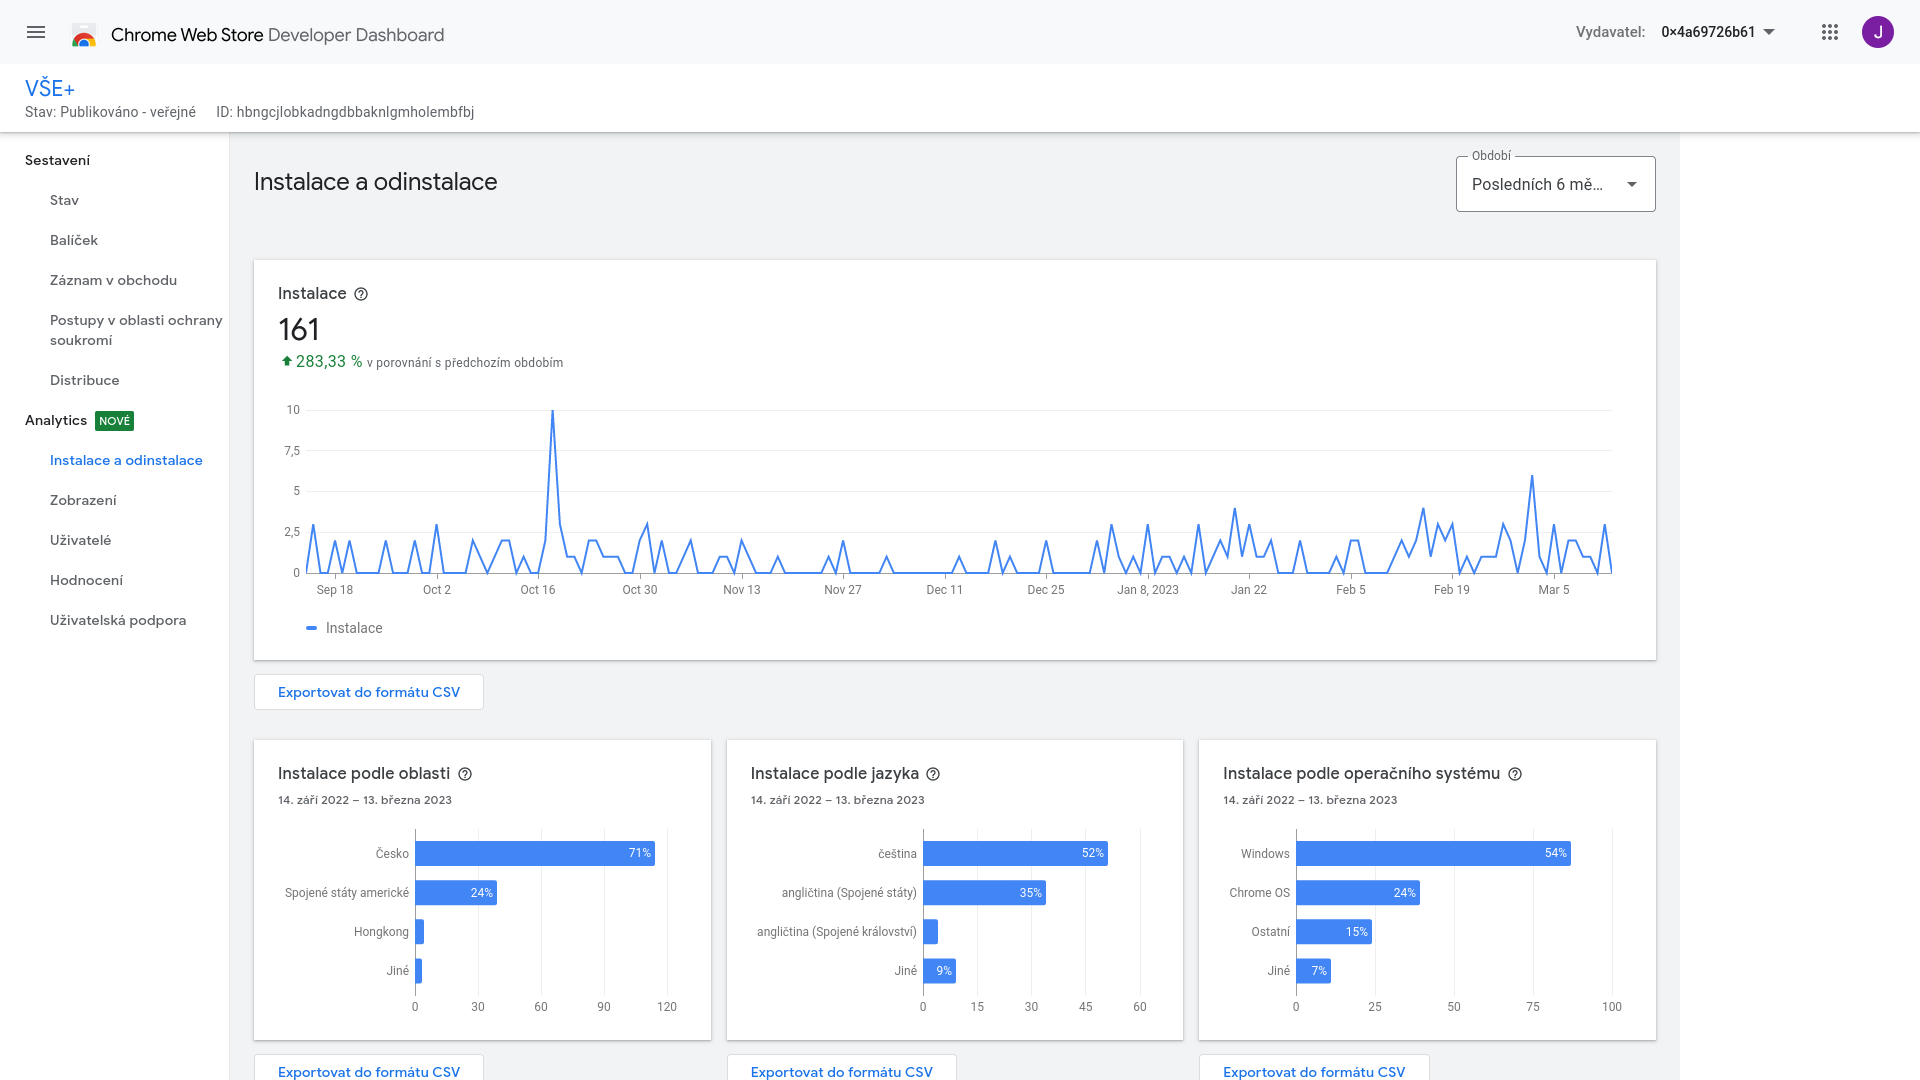
\includegraphics[width=\textwidth]{img/google-webstore-analytics.png}
% Příponu není potřeba explicitně uvádět, pdflatex automaticky hledá pdf.
% Rozměry také není nutné uvádět.
\caption{Statistiky v~panelu vývojáře v~rámci obchodu Google Web Store (vlastní zpracování)}
\label{obr:google-webstore-analytics}
\end{figure}

\subsection{Sestavování balíčků rozšíření}

Před publikací je nutné zkompilovat zdrojový kód společně s~manifestem rozšíření a~ostatními statickými soubory z~adresáře \url{public}. Výstupem sestavení je komprimovaný zip soubor, který v~kořenovém adresáři obsahuje soubor s~manifestem rozšíření a zkompilované zdrojové kódy.

V~rámci sestavování balíčku také dochází k~minimalizaci počtu sestavených souborů. K~tomu slouží takzvané bundlery, které umožňují zkombinovat více souborů do jednoho, který se označuje jako bundle. Dále tyto nástroje umí provést minifikaci výsledného kódu a optimalizaci závislostí. Pro sestavování bundle rozšíření VŠE+ byl zvolen nástroj Webpack, který je v~současnosti jedním z~nejrozšířenějších bundlerů. Jednou z~výhod tohoto bundleru je možnost extenzivní konfigurace pomocí JavaScript kódu, což umožňuje využití konstruktů programovacího jazyka JavaScript jako jsou cykly nebo kopozice funkcí při definici konfiguračních pravidel. Využití těchto syntaktických konstrukcí není monžé u~konfiguračních souborů ve formátech jako je například JSON nebo YAML.

V~rámci projektu jsou definované 2 webpack konfigurace pro sestavování balíčků, jedna pro sestavování během vývoje a jedna pro produkční sestavení. Tyto konfigurace se nachází v~souborech \code{webpack/webpack.dev.js} a \code{webpack/webpack.prod.js}. Dále se ve složce \code{webpack} nachází ještě soubor \code{webpack.common.js}, který obsahuje konfigurační pravidla, která jsou sdílená mezi produkční a vývojářskou verzí konfigurace. Cesta ke zvolenému konfiguračnímu souboru se předává programu \code{webpack} pomocí parametru \code{-{}-config}. Pro snazší práci s~předáváním konfiguračních souborů nástroji webpack byly definovány 2 aliasy v~sekci \code{scripts} souboru \code{package.json}.

\begin{lstlisting}[label={code:package-json-webpack-alias}, caption={Definice aliasů pro práci s~nástrojem webpack (vlastní zpracování)}]
"scripts": {
    "dev": "webpack --config webpack/webpack.dev.js --watch",
    "build": "webpack --config webpack/webpack.prod.js",
}
\end{lstlisting}

Definice aliasů viz výpis \ref{code:package-json-webpack-alias} umožňují sestavení balíčku pomocí nástroje webpack spouštět přes příkazy \code{npm run dev} pro vývojovou konfiguraci, respektive \code{npm run build} pro produkční konfiguraci. Parametr \code{-{}-watch} u~aliasu \code{dev} spustí webpack v~takzvaném watch módu, který spouští kompilaci po změně jakéhokoliv ze souborů, které webpack spravuje. To zásadním způsobem zvyšuje produktivitu při vývoji rozšíření, protože je možné ihned po úpravě zdrojového kódu pozorovat implementované změny bez nutnosti manuálního spouštění kompilace a sestavení balíčku.

Pro zjednodušení a automatizaci sestavování rozšíření do balíčku publikovatelného na zmíněné internetové obchody je využíváno GitLab CI/CD pipeline, která automaticky sestavuje balíčky a vytváří takzvané releases na platformě GitLab, ze kterých je možné tyto sestavené balíčky přímo publikovat na zmíněné internetové obchody s rozšířeními. 

Zdrojový kód této CI pipeline je možné vidět ve výpise \ref{code:gitlab-ci-pipeline} a snímek obrazovky z platformy GitLab s výsledkem běhu je možné vidět na obrázku \ref{fig:extension-gitlab-ci}.

\begin{figure}[htbp!]\centering
    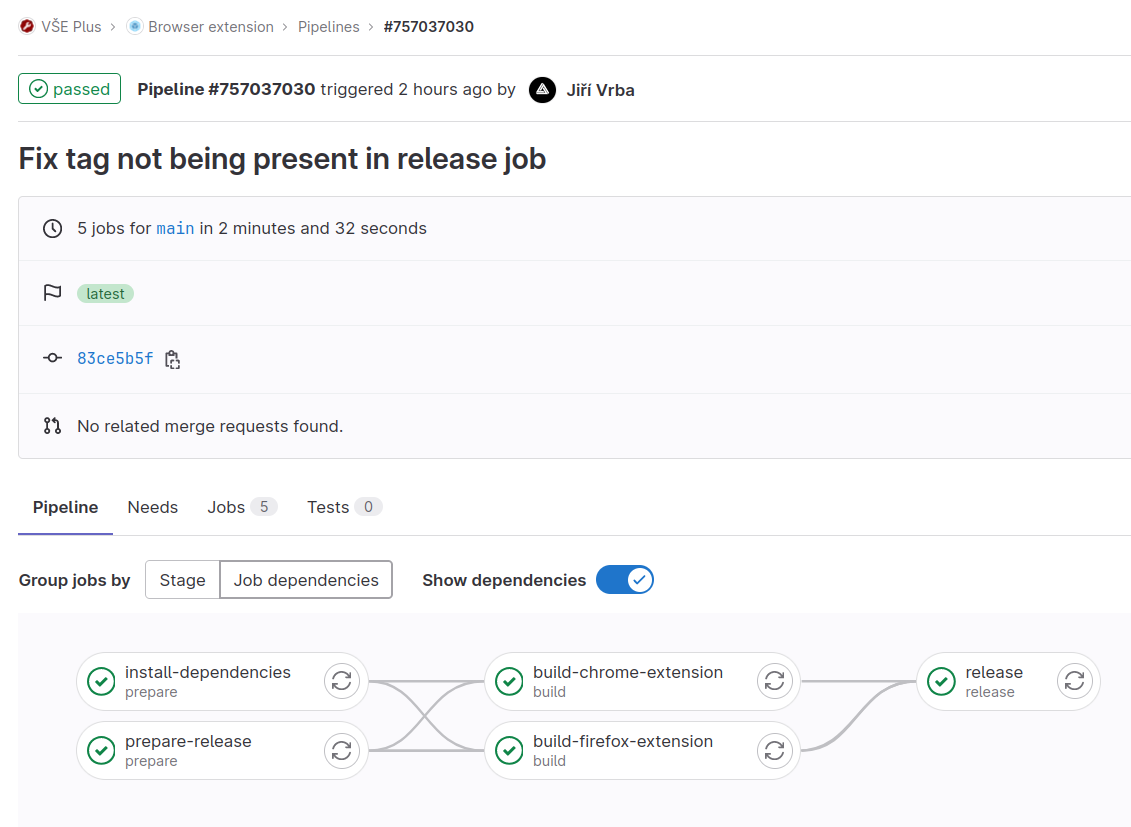
\includegraphics[width=\textwidth]{img/extension-gitlab-ci-pipeline-overview.png}
    \caption{GitLab CI Pipeline (vlastní zpracování)}
    \label{fig:extension-gitlab-ci}
\end{figure}

Aktuální verze kompletního zdrojového kódu včetně historie změn je dostupná v~podobě repozitáře na platformě GitLab na adrese \url{https://gitlab.com/vse-plus/extension}.

\chapter{Evaluace zpětné vazby od ostatních studentů VŠE}\label{chap:zpetna-vazba}

Tato kapitola se zabývá evaluací zpětné vazby od ostatních studentů Vysoké školy ekonomické v~Praze, která byla sesbírána pomocí metody dotazníkového šetření. Kapitola obsahuje proces za návrhem dotazníku

Pro sběr zpětné vazby od ostatních studentů Vysoké školy ekonomické v~Praze pro následnou evaluaci byla zvolena metoda dotazníkového šetření. Cílem dotazníku je lépe pochopit potřeby uživatelů webového rozšíření a zodpovědět stanovené výzkumné otázky.

Byly stanoveny následující výzkumné otázky, které jsou se dotazníkové šetření:

\begin{enumerate}
    \item Využívá většina uživatelů rozšíření rozšíření s~přihlášením?
    \item Využívá většina uživatelů rozšíření alespoň 2 přidané funkcionality?
    \item Odpovídají výsledky dotazníkového šetření počáteční analýze používání systému InSIS?
\end{enumerate}

\section{Návrh dotazníku}

Dotazník byl vytvořen prostřednictvím platformy Google Forms, která umožňuje jednoduchou editaci a zároveň poskytuje nástroje pro tvorbu komplexních dotazníků, jako větvení průchodu dotazníkem podle předchozích odpovědí respondenta. To je užitečné například pro zobrazení odlišných otázek respondentům, kteří rozšíření nepoužívají, aby byla zpětná vazba co nejrelevantnější. Nedávalo by smysl se respondentů, kteří rozšíření nepoužívají, ptát na dílčí funkcionality nebo se naopak dotazovat uživatelů, kteří rozšíření mají nainstalované, jaké jsou jejich primární důvody proč rozšíření nepoužívají. 

Celý dotazník je členěn do 8 sekcí, které se respondentům zobrazují v~závislosti na předchozích odpovědích. Každá část dotazníku obsahuje 1--20 otázek, které jsou buď výběr 1 nebo více možností z~předem stanoveného výběru nebo otevřené odpovědi s~doplněním vlastního textu. Schéma průchodu dotazníkem zobrazuje obrázek \ref{fig:dotaznik}.

\begin{figure}[htbp!]\centering
    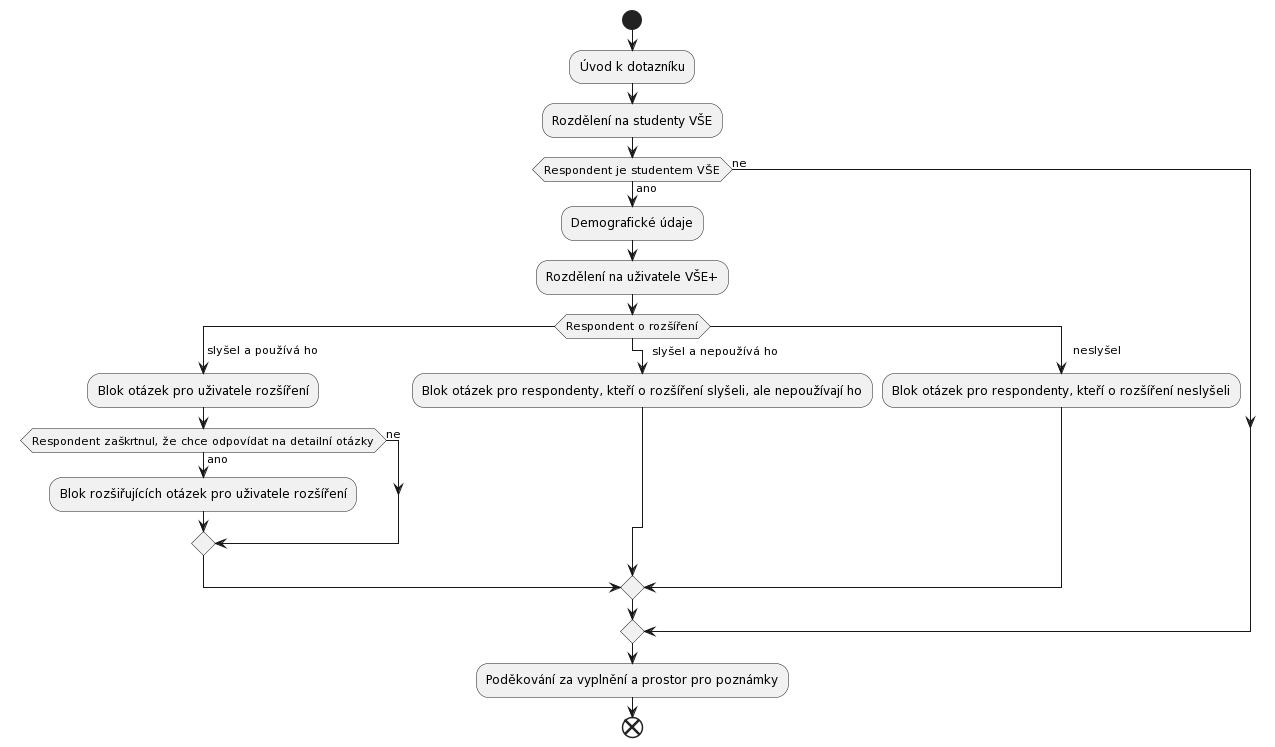
\includegraphics[width=\textwidth]{img/dotaznik.png}
    \caption{Schéma průchodu dotazníkem (vlastní zpracování)}
    \label{fig:dotaznik}
\end{figure}
\imagesource{
@startuml
start
:Úvod k~dotazníku;

:Rozdělení na studenty VŠE;

if (Respondent je studentem VŠE) then (ano)
  :Demografické údaje;
  :Rozdělení na uživatele VŠE+;
  switch (Respondent o~rozšíření) 
  case ( slyšel a používá ho) 
    :Blok otázek pro uživatele rozšíření;
    if (Respondent zaškrtnul, že chce odpovídat na detailní otázky) then (ano)
        :Blok rozšiřujících otázek pro uživatele rozšíření;
    else (ne)
    endif
  case (     slyšel a nepoužívá ho)
    :Blok otázek pro respondenty, kteří o~rozšíření slyšeli, ale nepoužívají ho;
  case (   neslyšel)
    :Blok otázek pro respondenty, kteří o~rozšíření neslyšeli;
  endswitch
else (ne)
endif

:Poděkování za vyplnění a prostor pro poznámky;
end
@enduml
}

\section{Představení dat}

Celkem bylo v~dotazníkovém šetření nasbíráno od respondentů 85 odpovědí. Z~tohoto celku je 74 odpovědí od respondentů, kteří jsou v~současné době studenty Vysoké školy ekonomické v~Praze a o~rozšíření VŠE+ slyšeli. Z~těchto 74 odpovědí pak 42 respondentů chtělo odpovídat na doplňující otázky ke každé z~implementovaných funkcionalit. Vzhledem k~počtu instalací webového rozšíření se jedná o~poměrně rozsáhlý vzorek uživatelů. 

\subsection{Demografie respondentů}

Jako relevantní demografické údaje sbírané od respondentů byly zvoleny údaje o~stupni vysokoškolského studia, ročníku a fakultě na které respondent studuje. Z~celkového počtu 74 respondentů bylo 71 respondentů z~fakulty informatiky a statistiky, což je pravděpodobně důsledkem zvolených způsobů sdílení formuláře.

Rozložení počtu respondentů vzhledem k~stupni vysokoškolského studia a ročníku je možné vidět na obrázku \ref{fig:demografie-respondentu}. Nejpočetnější skupinou respondentů v~tomto zobrazení jsou studenti 3. ročníku bakalářských studií, což může být opět důsledkem zvoleného způsobu sdílení formuláře. Zajímavým jevem, který je možné vypozorovat na obrázku \ref{fig:zdroj-instalace} je skutečnost, že studenti prvních a druhých ročníků se v~porovnání se studenty třetích ročníků o~rozšíření častěji dozvěděli z~doporučení od spolužáka, zatímco studenti třetích ročníků se nejčastěji o~rozšíření dozvěděli prostřednictvím neoficiálního fakultního serveru na chatovací platformě Discord. 

\begin{figure}[htbp!]\centering
    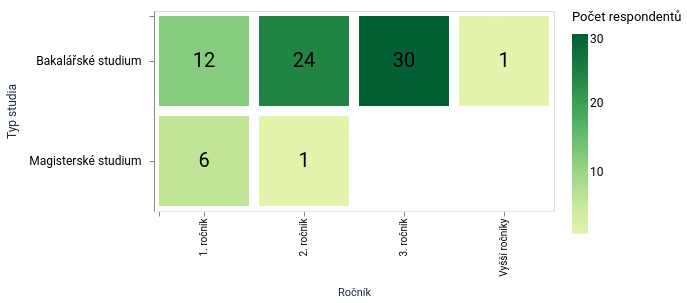
\includegraphics[width=\textwidth]{img/demografie-respondentu.png}
    \caption{Demografie respondentů dotazníkového šetření (vlastní zpracování)}
    \label{fig:demografie-respondentu}
\end{figure}

\begin{figure}[htbp!]\centering
    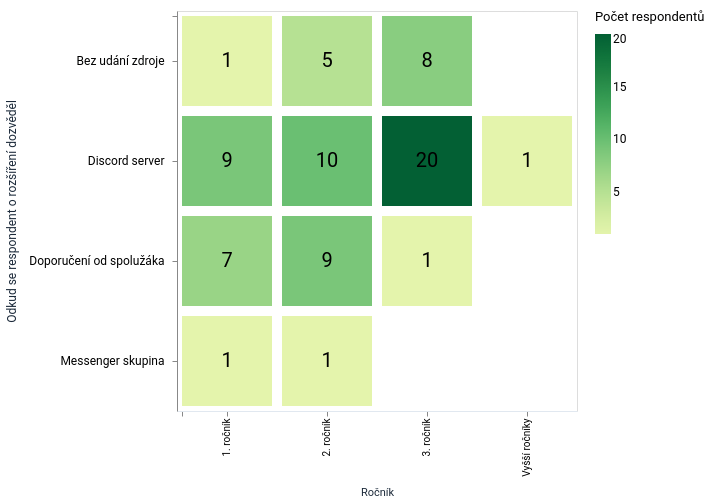
\includegraphics[width=\textwidth]{img/zdroj-instalace.png}
    \caption{Zdroje, ze kterých se respondenti o~rozšíření dozvěděli (vlastní zpracování)}
    \label{fig:zdroj-instalace}
\end{figure}

\subsection{Využívání přidaných funkcionalit}

Ve čtvrté sekci dotazníku všichni respondenti, kteří jsou současnými nebo bývalými studenty VŠE vybírali z~výběru 1 nebo více přidaných funkcionalit, které používají. Nasbírané statistiky od 60 respondentů zobrazuje graf na obrázku \ref{fig:features-data}. Z~odpovědí dále vyplývá, že 51 respondentů využívá funkcionalitu náhledu rozvrhu při registraci rozvrhových akcí, 38 respondentů využívá funkcionalitu připomínání odevzdáváren a 52 respondentů využívá funkcionalitu vylepšeného rozvrhu. 

\begin{figure}[htbp!]\centering
    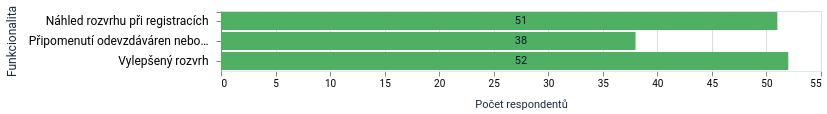
\includegraphics[width=\textwidth]{img/features.png}
    \caption{Statistiky využívání přidaných funkcionalit (vlastní zpracování)}
    \label{fig:features-data}
\end{figure}

\subsection{Evaluace zpětné vazby k~implementaci vylepšeného rozvrhu}

V~sekci dotazníku zaměřené na modul s~vylepšeným rozvrhem byly na respondenty kladeny 3 otázky týkající se využívání dílčích funkcionalit pro lepší pochopení interakce respondentů s~rozvrhem. Jak zobrazuje obrázek \ref{fig:timetable-feedback}, na otázku jestli respondenti využívají možnosti přepínání mezi jednotlivými týdny ve výukovém období 24 respondentů odpovědělo že ano a 18 respondentů odpovědělo že ne. Na otázku jestli respondenti využívají možnosti přidávání poznámek k~hodinám v~rozvrhu odpovědělo 6 respondentů ano a 36 respondentů ne. 

Toto bylo pro autora překvapivé zjištění, protože na základě analýzy práce s~rozvrhem studentů předcházející samotné implementaci rozšíření vyplynulo, že ostatní studenti mají podobný workflow práce s~rozvrhem jako autor. Výsledky dotazníkového šetření ovšem tento předpoklad vyvrací a namísto toho naznačují, že se chování ostatních uživatelů rozšíření liší od výsledku počáteční analýzy.

\begin{figure}[htbp!]\centering
    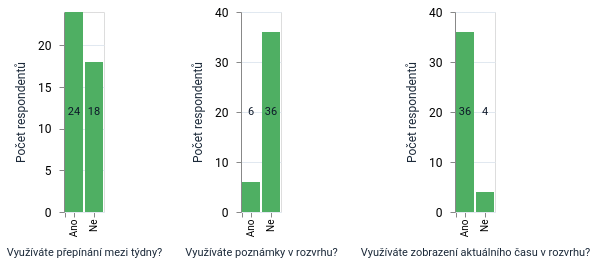
\includegraphics[width=\textwidth]{img/timetable.png}
    \caption{Využití dílčích částí vylepšeného rozvrhu (vlastní zpracování)}
    \label{fig:timetable-feedback}
\end{figure}

\subsection{Evaluace zpětné vazby k~implementaci připomenutí odevzdáváren}


V~sekci dotazníku se zpětnou vazbou k~implementaci připomínání odevzdáváren byly respondentům dotazníku kladeny 3 kvantitativní otázky. Tyto otázky byly definovány následovně:

\begin{enumerate}
    \item Využíváte možnost nechat si na odevzdávárny zaslat upozornění?
    \item Využíváte možnost exportovat odevzdávárny do Google kalendáře / Outlooku?
    \item Vyhovuje vám výběr časů před uzavřením odevzdávárny?
\end{enumerate}

Na každou z~otázek respondenti odpovídali buď ano nebo ne s~výjimkou 3. z~uvedených otázek, kde byla přidána do výběru možnost, že připomínání odevzdáváren respondent nevyužívá.

Kromě těchto 3 kvantitativních otázek byly v~této sekci definovány i 3 kvalitativní otázky, ve kterých respondenti odpovídali, jestli používají jiné platformy pro správu kalendáře kromě dvou již podporovaných platforem, jestli existuje nějaká skutečnost, která jim na implementaci této funkcionality vadí, a jestli jim naopak něco v~implementaci chybí.

\begin{figure}[htbp!]\centering
    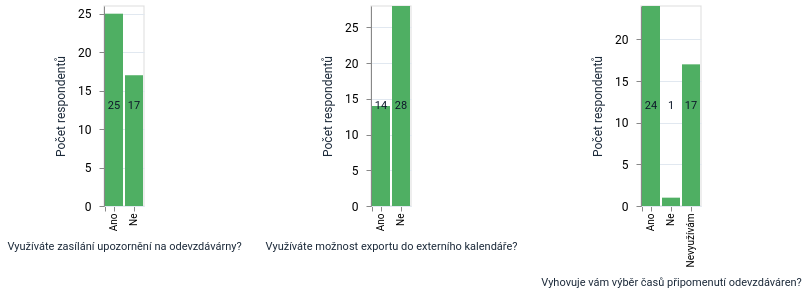
\includegraphics[width=\textwidth]{img/pripomenuti-vizualizace.png}
    \caption{Využití dílčích částí připomenutí odevzdáváren (vlastní zpracování)}
    \label{fig:pripomenuti-vizualizace}
\end{figure}

Odpovědi respondentů v~této sekci dotazníku odpovídají počáteční analýze, protože většina studentů využívá zasílání upozornění na email a pouze menšina využívá export do externího kalendáře. Pozitivní zpětnou vazbou bylo ověření vhodného výběru časů připomenutí, které vyhovovaly 24 z~25 uživatelům rozšíření, kteří funkcionalitu připomenutí odevzdáváren využívají.

\subsection{Evaluace zpětné vazby k~náhledu rozvrhu při registracích}

V~této sekci dotazníku byly na respondenty kladeny 2 kvantitativní otázky a podobně jako u~ostatních částí na dílčí funkcionality, také 2 kvalitativní otázky.

Cílem této části dotazníku bylo zhodnotit míru využívání náhledu rozvrhu při registraci předmětů a získat zpětnou vazbu k~implementaci vyznačování hodin s~kolizí v~rozvrhu. Hlavní zmiňovanou položkou při prvotních konzultacích s~uživateli rozšíření byla grafická stránka implementace, proto byly do možných odpovědí na otázku \quot{Pomáhá vám při registracích funkce detekcí kolizí v~rozvrhu?} přidány možnosti \quot{Ano, ale ocenil bych možnost vypnout grafické rozlišení} a \quot{Ano, ale změnil bych grafické rozlišení}.  

Odpovědi respondentů v~této sekci dotazníku odpovídají počáteční analýze, protože většina studentů využívá zasílání upozornění na email a pouze menšina využívá export do externího kalendáře. Pozitivní zpětnou vazbou bylo ověření vhodného výběru časů připomenutí, které vyhovovaly 24 z~25 uživatelům rozšíření, kteří funkcionalitu připomenutí odevzdáváren využívají.

\subsection{Evaluace zpětné vazby k~náhledu rozvrhu při registracích}

V~této sekci dotazníku byly na respondenty kladeny 2 kvantitativní otázky a podobně jako u~ostatních částí na dílčí funkcionality, také 2 kvalitativní otázky.

Cílem této části dotazníku bylo zhodnotit míru využívání náhledu rozvrhu při registraci předmětů a získat zpětnou vazbu k~implementaci vyznačování hodin s~kolizí v~rozvrhu. Hlavní zmiňovanou položkou při prvotních konzultacích s~uživateli rozšíření byla grafická stránka implementace, proto byly do možných odpovědí na otázku \quot{Pomáhá vám při registracích funkce detekcí kolizí v~rozvrhu?} přidány možnosti \quot{Ano, ale ocenil/a bych možnost vypnout grafické rozlišení} a \quot{Ano, ale změnil/a bych grafické rozlišení}.    

Graf na obrázku \ref{fig:nahledy-vizualizace} zachycuje zastoupení jednotlivých odpovědí na kvantitativní otázky.

\begin{figure}[htbp!]\centering
    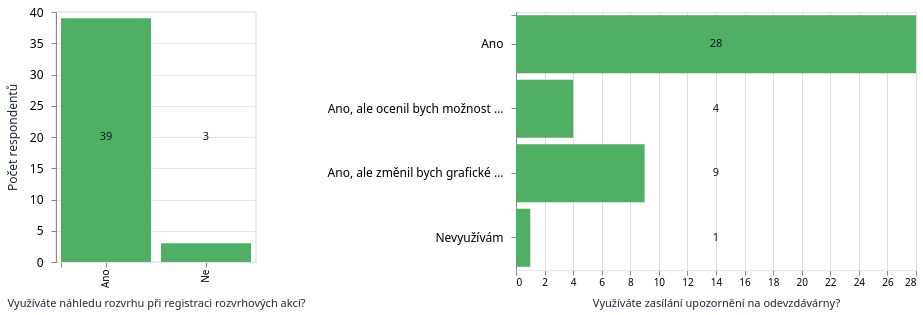
\includegraphics[width=\textwidth]{img/preview-visualization.png}
    \caption{Využití dílčích částí náhledu rozvrhů (vlastní zpracování)}
    \label{fig:nahledy-vizualizace}
\end{figure}

\section{Výsledky dotazníkového šetření}

Na základě odpovědí od respondentů dotazníkového šetření byly zodpovězeny výzkumné otázky, které byly stanovené na začátku kapitoly.

První výzkumná otázka \quot{Využívá většina uživatelů rozšíření rozšíření s~přihlášením?} byla zodpovězena ano, jelikož 86.7 \% respondentů, kteří odpověděli, že rozšíření používají, používá rozšíření s~aktivním přihlášením pomocí školního účtu.

Druhá výzkumná otázka \quot{Využíváte možnost exportovat odevzdávárny do Google kalendáře / Outlooku?} byla také zodpovězena ano, jelikož přes 83 \% respondentů, kteří odpověděli, že rozšíření používají, používá alespoň 2 z~přidaných funkcionalit.

Poslední výzkumná otázka \quot{Odpovídají výsledky dotazníkového šetření počáteční analýze používání systému InSIS?} je jedinou výzkumnou otázkou, která nebyla potvrzena. Důvodem je rozpor počáteční analýzy v~oblasti používání rozvrhu a předpokladu používání poznámek přímo v~rozvrhu a sesbíraných dat, která indikují pouze minimální využívání této přidané funkcionality. Chybná počáteční analýza používání rozvrhu mohla být způsobena omezeným vzorkem respondentů v~počáteční analýze.

% \include{...}
% \include{...}
{%
\pagestyle{plain}
\chapter*{Závěr}
\addcontentsline{toc}{chapter}{Závěr}

Předmětem této práce bylo navržení a následná implementace rozšíření do webových prohlížečů pro zjednodušení práce a zvýšení efektivity uživatelů integrovaného studijního informačního systému InSIS.

V práci byly navrženy 3 nové funkcionality, které byly následně v podobě rozšíření implementovány. První přidanou funkcionalitou je náhled rozvrhu při registraci rozvrhových akcí. Další přidanou funkcionalitou je správa a zasílání připomenutí na odevzdávárny s~blížícím se datem odevzdání, což bylo velice žádané rozšíření již existujícího modulu informačního systému InSIS. Poslední implementovanou funkcionalitou je vylepšená verze zobrazení aktuálního rozvrhu studenta, která oproti původní verzi přidává možnost přidávání poznámek ke konkrétním hodinám, přepínání mezi výukovými týdny nebo automatické zpracování volných dní a konání blokových akcí.

Prvním cílem práce byl návrh a implementace rozšíření do webových prohlížečů. Kapitola \ref{chap:navrh-a-specifikace} se zabývá návrhem výše zmíněných přidaných funkcionalit. V kapitolách \ref{chap:server} a \ref{chap:extension} je detailně popsán vývoj obou dílčích částí softwarového řešení. První z těchto částí je podpůrný webový server, který byl implementován, otestován a nasazen na platformě Digital Ocean. Druhá část, tedy samotné rozšíření do webových prohlížečů je navržené tak, aby bylo snadné do budoucna přidávat další funkcionality nebo měnit současnou podobu přidaných funkcionalit. Podpůrný webový server je distribuován v podobě Docker kontejneru, který je možné snadno přenášet mezi hostingovými platformami v případě změny požadavků na dostupný výpočetní výkon. 

Druhým cílem práce bylo porovnání a výběr technologií pro implementaci obou částí řešení. Kapitola \ref{chap:volba-technologii} představuje některé z dostupných technologií a jejich srovnání v~příslušném kontextu. Pro vývoj rozšíření do webových prohlížečů byl zvolen programovací jazyk TypeScript a knihovna React.js společně se sadou komponent Chakra UI. Pro podpůrný webový server byl zvolen aplikační rámec Spring s nadstavbou Spring Boot společně s programovacím jazykem Kotlin a systémem řízení báze dat PostgreSQL. 

Poslední cílem práce byla evaluace zpětné vazby od ostatních studentů, kteří rozšíření používají. V~kapitole \ref{chap:zpetna-vazba} bylo vyhodnoceno dotazníkové šetření, které odpovídalo na 3 stanovené výzkumné otázky. Návrhu rozšíření předcházela analýza používání systému InSIS jeho uživateli. Účelem výzkumných otázek stanovených v kapitole \ref{chap:zpetna-vazba} je vyhodnotit míru shody této počáteční analýzy s používáním výslené podoby rozšíření. Provedené dotazníkové šetření zároveň poskytuje autorovi přímou zpětnou vazbu v podobě odpovědí na kvalitativní otázky.

Všechny vymezené cíle práce byly splněny a výsledkem práce je funkční rozšíření do webových prohlížečů, které je publikováno na internetových obchodech Google Web Store a Firefox Addons. V~době psaní má rozšíření do prohlížečů přes 300 instalací a více než 120 aktivních uživatelů. 

\clearpage
Do budoucna by bylo možné na tuto práci navázat především přidáním podpory pro další webové prohlížeče, zejména Apple Safari, který je výchozím webovým prohlížečem v operačním systému macOS, který řada studentů používá. Dále by bylo možné přidat dokumentaci a uživatelský manuál pro zjednodušení orientace nových uživatelů v přidaných funkcionalitách. Před přidáním dalších funkcionalit do rozšíření by bylo vhodné rozšířit povědomí o existenci rozšíření a tím zvýšit počet jeho uživatelů a tedy i vzorku respondentů pro budoucí dotazníková šetření. 

}

%%% Seznam použité literatury
%%% Bibliography
%% Toto platí v případě použití samostatné bibliografické databáze
\printbibliography[title={\bibname},heading={bibintoc}]

%% Toto platí v případě použití prostředí thebibliography
%% Pro sestavení citačních údajů lze doporučit:
%%     https://knihovna.vse.cz/citace/priklady/
%%     https://www.citace.com/
%\openright
%\phantomsection
%\addcontentsline{toc}{chapter}{\bibname}
%\begin{thebibliography}{99}
%\bibitem{Cermak2018}ČERMÁK, Radim, SMUTNÝ, Zdeněk. A Framework for Cultural Localization of Websites and for Improving Their Commercial Utilization. In:  \emph{Global Observations of the Influence of Culture on Consumer Buying Behavior} [online]. Hershey~: IGI Global, 2018, s. 206--232. ISBN 978-1-5225-2727-5. DOI: 10.4018/978-1-5225-2727-5.
%
%\bibitem{Hladik2018}HLADÍK, Milan, ČERNÝ, Michal. The Shape of the Optimal Value of a Fuzzy Linear Programming Problem. In: \emph{Fuzzy Logic in Intelligent System Design} [online]. Cancum, 16.10.2017 -- 18.10.2017. Cham~: Springer, 2018, s. 281--286. Advances in Intelligent Systems and Computing 648. ISBN 978-3-319-67136-9. DOI: 10.1007/978-3-319-67137-6\_31.
%
%\bibitem{Jasek2018}JAŠEK, Pavel, VRANÁ, Lenka, ŠPERKOVÁ, Lucie, SMUTNÝ, Zdeněk, KOBULSKÝ, Marek. Modeling and Application of Customer Lifetime Value in Online Retail. \emph{Informatics} [online]. 2018, roč. 5, č. 1. 22 s. eISSN 2227-9709. DOI: 10.3390/informatics5010002. Dostupné také z: \url{http://www.mdpi.com/2227-9709/5/1/2/pdf}.
%
%\bibitem{Pecakova2018}PECÁKOVÁ, Iva. \emph{Statistika v terénních průzkumech}. 3. přeprac. vyd. Praha~: Professional Publishing, 2018. 254 s. ISBN 978-80-88260-10-3.
%\end{thebibliography}


%%% Přílohy k práci, existují-li. Každá příloha musí být alespoň jednou
%%% odkazována z vlastního textu práce. Přílohy se číslují.
%%% Attachments to thesis, if any. Each attachment must be referenced at 
%%% least once in your own text. The appendices are numbered.
\part*{\Prilohy\thispagestyle{empty}}
\appendix
\chapter{Formulář v~plném znění}


\chapter{Zdrojové kódy výpočetních procedur}

\begin{lstlisting}[label={code:liquibase-changelog}, caption={SQL soubor s migracemi pro nástroj Liquibase (vlastní zpracování)}]
--liquibase formatted sql

--changeset jirkavrba:create-accounts-table
create table accounts
(
    id int not null generated by default as identity primary key,
    username varchar(6) not null unique,
    verification_code varchar(8) null
);

--changeset jirkavrba:create-submission-reminders-table
create table submission_reminders
(
    id int not null generated by default as identity primary key,
    account_id int not null,
    submission_id int not null, -- internal ID used by InSIS
    submission_name varchar(128) not null,
    submission_course varchar(128) not null,
    submission_due timestamp with time zone not null,
    reminder_date timestamp with time zone not null
);

alter table submission_reminders
    add constraint fk_submission_reminders_account_id 
    foreign key (account_id) references accounts (id) 
    on delete cascade;

--changeset jirkavrba:create-timetable-events-table
create table timetable_events
(
    id int not null generated by default as identity primary key,
    account_id int not null,
    entry_datetime timestamp with time zone not null,
    entry_course varchar(128) not null,
    event_type varchar(128) not null,
    event_note varchar(1024) not null
);

--changeset jirkavrba:create-notifications-table
create table notifications
(
    id int not null generated by default as identity primary key,
    published_on timestamp with time zone not null,
    notification_text varchar(1024) not null,
    notification_link varchar(1024)
);
\end{lstlisting}

\begin{lstlisting}[label={code:timetable-event-domain-class}, caption={Zdrojový kód doménové třídy \code{TimetableEvent}}]
package dev.vrba.vseplus.api.domain

import org.springframework.data.annotation.Id
import org.springframework.data.relational.core.mapping.Column
import org.springframework.data.relational.core.mapping.Table
import java.time.LocalDateTime

@Table("timetable_events")
data class TimetableEvent(
    @Id
    val id: Int = 0,

    @Column("account_id")
    val account: Int,

    @Column("entry_datetime")
    val datetime: LocalDateTime,

    @Column("entry_course")
    val course: String,

    @Column("event_type")
    val type: String,

    @Column("event_note")
    val note: String
)
\end{lstlisting}

\begin{lstlisting}[label={code:timetable-events-repository}, caption={Definice repozitáře pro doménovou třídu \code{TimetableEvent}}]
package dev.vrba.vseplus.api.repository

import dev.vrba.vseplus.api.domain.TimetableEvent
import kotlinx.coroutines.flow.Flow
import org.springframework.data.repository.kotlin.CoroutineCrudRepository
import org.springframework.stereotype.Repository

@Repository
interface TimetableEventsRepository : CoroutineCrudRepository<TimetableEvent, Int> {

    suspend fun findAllByAccount(account: Int): Flow<TimetableEvent>

    suspend fun findByIdAndAccount(id: Int, account: Int): TimetableEvent?

}
\end{lstlisting}

\begin{lstlisting}[label={code:gitlab-ci-pipeline}, caption={Definice GitLab CI/CD pipeline pro sestavování balíčků rozšíření (vlastní zpracování)}]
stages:
  - prepare
  - build
  - release

prepare-release:
  stage: prepare
  image: registry.gitlab.com/gitlab-org/release-cli:latest
  script:
    - echo "TAG=v$(cat VERSION)" >> variables.env
  artifacts:
    reports:
      dotenv: variables.env
  only:
    changes:
      - VERSION
    refs:
      - main

install-dependencies:
  stage: prepare
  image: node:alpine
  script:
    - npm install
  artifacts:
    expire_in: 1 hour
    paths:
      - node_modules
  cache:
    key:
      files:
        - package-lock.json
    paths:
      - node_modules
  only:
    changes:
      - VERSION
    refs:
      - main
    
build-chrome-extension:
  stage: build
  image: node:alpine
  script:
    - apk add zip
    - npm run chrome
    - npm run build
    - rm ./dist/manifest-chrome.json
    - rm ./dist/manifest-firefox.json
    - cd dist
    - zip ../extension-chrome.zip -r ./*
  needs:
    - install-dependencies
    - prepare-release
  artifacts:
    expire_in: 1 hour
    paths:
      - ./extension-chrome.zip
  only:
    changes:
      - VERSION
    refs:
      - main
    
build-firefox-extension:
  stage: build
  image: node:alpine
  script:
    - apk add zip
    - npm run firefox
    - npm run build
    - rm ./dist/manifest-chrome.json
    - rm ./dist/manifest-firefox.json
    - cd dist
    - zip ../extension-firefox.zip -r ./*
  needs:
    - install-dependencies
    - prepare-release
  artifacts:
    expire_in: 1 hour
    paths:
      - ./extension-firefox.zip
  only:
    changes:
      - VERSION
    refs:
      - main

release:
  stage: release
  image: registry.gitlab.com/gitlab-org/release-cli:latest
  only:
    changes:
      - VERSION
    refs:
      - main
  script:
    - echo "Creating release for $TAG"
    - mkdir output
    - cp ./extension-chrome.zip ./output/extension-chrome-$TAG.zip
    - cp ./extension-firefox.zip ./output/extension-firefox-$TAG.zip
  artifacts:
    paths:
     - output
  release:
    name: "Release $TAG"
    description: "Automatically generated release for the version $TAG"
    tag_name: "$TAG"
    ref: "$CI_COMMIT_SHA"
    assets:
      links:
        - name: Chrome extension
          url: $CI_JOB_URL/artifacts/raw/output/extension-chrome-$TAG.zip
        - name: Firefox extension
          url: $CI_JOB_URL/artifacts/raw/output/extension-firefox-$TAG.zip
  needs:
    - build-firefox-extension
    - build-chrome-extension
    - prepare-release
\end{lstlisting}

\begin{lstlisting}[label={code:gitlab-ci-docker}, caption={GitLab CI/CD pipeline pro sestavování a publikaci docker image (vlastní zpracování)}]
stages:
  - test
  - prepare
  - build
  - release

prepare-release:
  stage: prepare
  image: registry.gitlab.com/gitlab-org/release-cli:latest
  script:
    - echo "VERSION=$(cat gradle.properties | sed 's/^apiVersion=//')" >> variables.env
    - echo "TAG=v$(cat gradle.properties | sed 's/^apiVersion=//')" >> variables.env
  artifacts:
    reports:
      dotenv: variables.env

run-tests:
  stage: test
  image: docker:23.0.1-dind-alpine3.17 # Needs docker-in-docker for running test containers
  services:
    - docker:23.0.1-dind
  before_script:
    - apk add --update openjdk17
    - export GRADLE_USER_HOME=`pwd`/.gradle
  script:
    - chmod 755 ./gradlew
    - ./gradlew test
  cache:
    paths:
      - build
      - .gradle/wrapper
      - .gradle/caches
    key:
      files:
        - build.gradle.kts
        - settings.gradle.kts
  artifacts:
    reports:
      junit:
        - build/test-results/test/TEST-*.xml

build-docker-image:
  stage: build
  image: docker:23.0.1-dind-alpine3.17
  needs:
    - prepare-release
  services:
    - docker:23.0.1-dind
  before_script:
    - apk add --update openjdk17
    - export GRADLE_USER_HOME=`pwd`/.gradle
    - docker login -u $CI_REGISTRY_USER -p $CI_REGISTRY_PASSWORD $CI_REGISTRY
  script:
    - chmod 755 ./gradlew
    - ./gradlew bootBuildImage
    - docker push $CI_REGISTRY_IMAGE:$VERSION
  only:
    changes:
      - gradle.properties
    refs:
      - main
  cache:
    paths:
      - build
      - .gradle/wrapper
      - .gradle/caches
    key:
      files:
        - build.gradle.kts
        - settings.gradle.kts
    
release:
  stage: release
  image: registry.gitlab.com/gitlab-org/release-cli:latest
  needs:
    - prepare-release
  only:
    changes:
      - gradle.properties
    refs:
      - main
  script:
    - echo "Creating release for $TAG"
  release:
    name: "Release $TAG"
    description: "Automatically generated release for the version $TAG"
    tag_name: "$TAG"
    ref: "$CI_COMMIT_SHA"
\end{lstlisting}

\begin{lstlisting}[label={code:accounts-controller}, caption={Definice třídy kontroleru pro uživatelské účty}]
package dev.vrba.vseplus.api.controller.api

import dev.vrba.vseplus.api.request.authentication.CreateAccountRequest
import dev.vrba.vseplus.api.request.authentication.VerifyAccountRequest
import dev.vrba.vseplus.api.response.authentication.CreateAccountResponse
import dev.vrba.vseplus.api.response.authentication.VerifyAccountResponse
import dev.vrba.vseplus.api.service.AccountService
import jakarta.validation.Valid
import org.springframework.http.HttpStatus
import org.springframework.http.ResponseEntity
import org.springframework.web.bind.annotation.PostMapping
import org.springframework.web.bind.annotation.RequestBody
import org.springframework.web.bind.annotation.RequestMapping
import org.springframework.web.bind.annotation.RestController

@RestController
@RequestMapping("/api/v1/account")
class AccountController(private val service: AccountService) {

    @PostMapping("/create")
    suspend fun createAccount(@Valid @RequestBody request: CreateAccountRequest): ResponseEntity<CreateAccountResponse> {
        val account = service.createAccount(request.username)
        val response = CreateAccountResponse(
            username = account.username,
            message = "Na email ${account.email} byl zaslán ověřovací kód"
        )

        return ResponseEntity.ok(response)
    }

    @PostMapping("/verify")
    suspend fun verifyAccount(@Valid @RequestBody request: VerifyAccountRequest): ResponseEntity<VerifyAccountResponse> {
        val token = service.verifyAccount(request.username, request.code) ?: return ResponseEntity.status(HttpStatus.UNPROCESSABLE_ENTITY).build()
        val response = VerifyAccountResponse(
            username = request.username,
            token = token
        )

        return ResponseEntity.ok(response)
    }
}
\end{lstlisting}

\begin{lstlisting}[label={code:create-account-request}, caption={Definice třídy \code{CreateAccountRequest} sloužící pro přenos dat}]
package dev.vrba.vseplus.api.request.authentication

import jakarta.validation.constraints.NotBlank
import jakarta.validation.constraints.Pattern
import jakarta.validation.constraints.Size

class CreateAccountRequest(
    @field:NotBlank
    @field:Size(min = 6, max = 6)
    @field:Pattern(regexp = "^[a-z]+[a-z0-9]+$")
    val username: String
)
\end{lstlisting}

\begin{lstlisting}[label={code:create-account-response}, caption={Definice třídy \code{CreateAccountResponse} sloužící pro přenos dat}]
package dev.vrba.vseplus.api.response.authentication

data class CreateAccountResponse(
    val username: String,
    val message: String
)
\end{lstlisting}

% \include{...}
% \include{...}

\end{document}
